% !TeX encoding = UTF-8
% !TeX program = xelatex
% !TeX spellcheck = en_US

\documentclass[degree=bachelor]{thuthesis}
\usepackage{listings}
\usepackage{xcolor}
\renewcommand{\lstlistingname}{清单}
\usepackage{enumitem}
\usepackage{pgfplots}
\usepackage{tikz} 
\usepackage{algorithmic}
\usepackage{graphicx}
\usetikzlibrary{shapes,calc,backgrounds,positioning,arrows.meta,patterns}
\usepackage{flushend}
  
\definecolor{myYellow}{RGB}{253, 231, 37}  
\definecolor{myLime}{RGB}{173,220,48}  
\definecolor{myGreen}{RGB}{94,201, 98}  
\definecolor{myGreenish}{RGB}{40,174,128}  
\definecolor{myTeal}{RGB}{33, 145, 140}  
\definecolor{myOcean}{RGB}{44,114,142}  
\definecolor{myBlue}{RGB}{59, 82, 139}  
\definecolor{myPurple}{RGB}{71,45,123}  
\definecolor{myEggplant}{RGB}{68, 1, 84}  
\pgfplotsset{compat=1.18}  
\usepgfplotslibrary{colormaps}  
\pgfplotsset{/pgfplots/bar cycle list/.style={/pgfplots/cycle list={%  
    {myTeal,fill=myTeal!80!white,mark=none,postaction={pattern=north west lines, pattern color=myTeal!70!black}},%  
    {myEggplant!60!black,fill=myEggplant!80!white,mark=none,postaction={pattern=north east lines, pattern color=myEggplant!70!black}},
    {myYellow,fill=myYellow!80!white,mark=none,postaction={pattern=crosshatch,pattern color=myYellow!70!black}},
    {myGreen,fill=myGreen!80!white,mark=none,postaction={pattern=vertical,pattern color=myGreen!70!black}},  
    {myblue,fill=myBlue!80!white,mark=none,postaction={pattern=grid,pattern color=myBlue!70!black}},  
},},}                            
  
\pgfplotsset{
    ourybarstyle/.style={
        axis x line*=bottom,  
        axis y line*=left,           
        ymin=0,  
        xtick=data,  
        ylabel style={at={(yticklabel* cs:1)}, anchor=south east, rotate=-90},  
        nodes near coords,  
        nodes near coords align={vertical},  
    },  
    ourbarstylenonums/.style={
        axis x line*=bottom,  
        axis y line*=left,           
        ymin=0,  
        xtick=data,  
        ylabel style={at={(yticklabel* cs:1)}, anchor=south east, rotate=-90},  
    },
    ourlinestyle/.style={
        ymin=0,  
    },  
}  

\setlength{\columnsep}{0.24 in}

\lstset{
    basicstyle=\ttfamily\small,
    commentstyle=\color{gray},
    keywordstyle=\color{blue},
    stringstyle=\color{red},
    breaklines=true,
    frame=single,
    numbers=none,
    numberstyle=\tiny\color{gray},
    captionpos=b
}

  % 学位 degree:
  %   doctor | master | bachelor | postdoc
  % 学位类型 degree-type:
  %   academic(默认)| professional
  % 语言 language
  %   chinese(默认)| english
  % 字体库 fontset
  %   windows | mac | fandol | ubuntu
  % 建议终版使用 Windows 平台的字体编译


% 论文基本配置,加载宏包等全局配置
% !TeX root = ./thuthesis-example.tex

% 论文基本信息配置

\thusetup{
  %******************************
  % 注意:
  %   1. 配置里面不要出现空行
  %   2. 不需要的配置信息可以删除
  %   3. 建议先阅读文档中所有关于选项的说明
  %******************************
  %
  % 输出格式
  %   选择打印版(print)或用于提交的电子版(electronic),前者会插入空白页以便直接双面打印
  %
  output = print,
  % 格式类型
  %   默认为论文(thesis),也可以设置为开题报告(proposal)
  % thesis-type = proposal,
  %
  % 标题
  %   可使用“\\”命令手动控制换行
  %
  title  = {操作系统宏内核内存管理模块的设计与实现},
  title* = {Design and Implementation of the Macro Kernel Memory Management Module in Operating System},
  %
  % 学科门类
  %   1. 学术型
  %      - 中文
  %        需注明所属的学科门类,例如:
  %        哲学、经济学、法学、教育学、文学、历史学、理学、工学、农学、医学、
  %        军事学、管理学、艺术学
  %      - 英文
  %        博士:Doctor of Philosophy
  %        硕士:
  %          哲学、文学、历史学、法学、教育学、艺术学门类,公共管理学科
  %          填写“Master of Arts“,其它填写“Master of Science”
  %   2. 专业型
  %      直接填写专业学位的名称,例如:
  %      教育博士、工程硕士等
  %      Doctor of Education, Master of Engineering
  %   3. 本科生不需要填写
  %
  % degree-category  = {工学硕士},
  % degree-category* = {Master of Science},
  %
  % 培养单位
  %   填写所属院系的全名
  %
  department = {计算机科学与技术系},
  %
  % 学科
  %   1. 研究生学术型学位,获得一级学科授权的学科填写一级学科名称,其他填写二级学科名称
  %   2. 本科生填写专业名称,第二学位论文需标注“(第二学位)”
  %
  discipline  = {计算机科学与技术},
  discipline* = {Computer Science and Technology},
  %
  % 专业领域
  %   1. 设置专业领域的专业学位类别,填写相应专业领域名称
  %   2. 2019 级及之前工程硕士学位论文,在 `engineering-field` 填写相应工程领域名称
  %   3. 其他专业学位类别的学位论文无需此信息
  %
  % professional-field  = {计算机技术},
  % professional-field* = {Computer Technology},
  %
  % 姓名
  %
  author  = {陈羿华},
  author* = {Chen Yihua},
  %
  % 学号
  % 仅当书写开题报告时需要(同时设置 `thesis-type = proposal')
  %
  % student-id = {2000310000},
  %
  % 指导教师
  %   中文姓名和职称之间以英文逗号“,”分开,下同
  %
  supervisor  = {陈渝, 副教授},
  supervisor* = {Associate Professor Chen Yu},
  %
  % 副指导教师
  %
  % associate-supervisor  = {陈文光, 教授},
  % associate-supervisor* = {Professor Chen Wenguang},
  %
  % 联合指导教师
  %
  % co-supervisor  = {某某某, 教授},
  % co-supervisor* = {Professor Mou Moumou},
  %
  % 日期
  %   使用 ISO 格式;默认为当前时间
  %
  % date = {2019-07-07},
  %
  % 是否在中文封面后的空白页生成书脊(默认 false)
  %
  include-spine = false,
  %
  % 密级和年限
  %   秘密, 机密, 绝密
  %
  % secret-level = {秘密},
  % secret-year  = {10},
  %
  % 博士后专有部分
  %
  % clc                = {分类号},
  % udc                = {UDC},
  % id                 = {编号},
  % discipline-level-1 = {计算机科学与技术},  % 流动站(一级学科)名称
  % discipline-level-2 = {系统结构},          % 专业(二级学科)名称
  % start-date         = {2011-07-01},        % 研究工作起始时间
}

% 载入所需的宏包

% 定理类环境宏包
\usepackage{amsthm}
% 也可以使用 ntheorem
% \usepackage[amsmath,thmmarks,hyperref]{ntheorem}

\thusetup{
  %
  % 数学字体
  % math-style = GB,  % GB | ISO | TeX
  math-font  = xits,  % stix | xits | libertinus
}

% 可以使用 nomencl 生成符号和缩略语说明
% \usepackage{nomencl}
% \makenomenclature

% 表格加脚注
\usepackage{threeparttable}

% 表格中支持跨行
\usepackage{multirow}

% 固定宽度的表格。
% \usepackage{tabularx}

% 跨页表格
\usepackage{longtable}

% 算法
\usepackage{algorithm}
\usepackage{algorithmic}

% 量和单位
\usepackage{siunitx}

% 参考文献使用 BibTeX + natbib 宏包
% 顺序编码制
\usepackage[sort]{natbib}
\bibliographystyle{thuthesis-numeric}

% 著者-出版年制
% \usepackage{natbib}
% \bibliographystyle{thuthesis-author-year}

% 生命科学学院要求使用 Cell 参考文献格式(2023 年以前使用 author-date 格式)
% \usepackage{natbib}
% \bibliographystyle{cell}

% 本科生参考文献的著录格式
% \usepackage[sort]{natbib}
% \bibliographystyle{thuthesis-bachelor}

% 参考文献使用 BibLaTeX 宏包
% \usepackage[style=thuthesis-numeric]{biblatex}
% \usepackage[style=thuthesis-author-year]{biblatex}
% \usepackage[style=gb7714-2015]{biblatex}
% \usepackage[style=apa]{biblatex}
% \usepackage[style=mla-new]{biblatex}
% 声明 BibLaTeX 的数据库
% \addbibresource{ref/refs.bib}

% 定义所有的图片文件在 figures 子目录下
\graphicspath{{figures/}}

% 数学命令
\makeatletter
\newcommand\dif{%  % 微分符号
  \mathop{}\!%
  \ifthu@math@style@TeX
    d%
  \else
    \mathrm{d}%
  \fi
}
\makeatother

% hyperref 宏包在最后调用
\usepackage{hyperref}



\begin{document}

% 封面
% \thusetup{
%     title = {操作系统宏内核内存管理模块接口的设计与实现},
%     author = {陈羿华},
%     department = {计算机科学与技术系},
%     discipline = {计算机科学与技术},
%     supervisor = {陈渝, 副教授},
% }
\maketitle


% 学位论文指导小组、公开评阅人和答辩委员会名单
% 本科生不需要
% % !TeX root = ../cyh.tex

\begin{committee}[name={学位论文指导小组、公开评阅人和答辩委员会名单}]

  \newcolumntype{C}[1]{@{}>{\centering\arraybackslash}p{#1}}

  \section*{指导小组名单}

  \begin{center}
    \begin{tabular}{C{3cm}C{3cm}C{9cm}@{}}
      李XX & 教授     & 清华大学 \\
      王XX & 副教授   & 清华大学 \\
      张XX & 助理教授 & 清华大学 \\
    \end{tabular}
  \end{center}


  \section*{公开评阅人名单}

  \begin{center}
    \begin{tabular}{C{3cm}C{3cm}C{9cm}@{}}
      刘XX & 教授   & 清华大学                    \\
      陈XX & 副教授 & XXXX大学                    \\
      杨XX & 研究员 & 中国XXXX科学院XXXXXXX研究所 \\
    \end{tabular}
  \end{center}


  \section*{答辩委员会名单}

  \begin{center}
    \begin{tabular}{C{2.75cm}C{2.98cm}C{4.63cm}C{4.63cm}@{}}
      主席 & 赵XX                  & 教授                    & 清华大学       \\
      委员 & 刘XX                  & 教授                    & 清华大学       \\
          & \multirow{2}{*}{杨XX} & \multirow{2}{*}{研究员} & 中国XXXX科学院 \\
          &                       &                         & XXXXXXX研究所  \\
          & 黄XX                  & 教授                    & XXXX大学       \\
          & 周XX                  & 副教授                  & XXXX大学       \\
      秘书 & 吴XX                  & 助理研究员              & 清华大学       \\
    \end{tabular}
  \end{center}

\end{committee}



% 也可以导入 Word 版转的 PDF 文件
% \begin{committee}[file=figures/committee.pdf]
% \end{committee}


% 使用授权的说明
% 本科生开题报告不需要
\copyrightpage
% 将签字扫描后授权文件 scan-copyright.pdf 替换原始页面
% \copyrightpage[file=scan-copyright.pdf]

\frontmatter
% !TeX root = ../cyh.tex

% 中英文摘要和关键字

\begin{abstract}
  内核是作为操作系统的核心组件,负责管理计算机系统的处理器、内存、文件系统等资源,
  其设计和实现对于操作系统的性能和稳定性至关重要。而模块化或者说组件化的内核设计则可以
  提高内核的可维护性和扩展性,同时也可以减少内核的复杂性和风险。

  内存管理模块是模块化内核设计中最基本的模块之一,其主要任务是管理计算机系统的内存资源,
  提供内存分配、释放和映射等功能。
  本文基于 ArceOs 基座和已有架构,对 starry-next 的内存管理模块进行详细地分析和设计,
  包括 ArceOs 内存管理相关的组件和模块、starry-next 内存管理模块的结构和内存管理机制,
  以及 mmap、munmap、mprotect、brk 等系统调用的实现与测试,验证了当前内存管理模块设计的
  正确性和稳定性,一定程度上明确了内存管理模块的功能与边界。
  
  同时,本文与该课题下其他模块共同开发宏内核的过程,也体现了内核的模块化设计
  在减少相互依赖、降低系统复杂度等方面的重要作用,为进一步的内核设计和优化提供了重要的参考和借鉴。

  % 关键词用“英文逗号”分隔,输出时会自动处理为正确的分隔符
  \thusetup{
    keywords = {操作系统, 内核, 内存管理, 模块化, 系统调用},
  }
\end{abstract}

\begin{abstract*}
  The kernel serves as the core component of an operating system, 
  tasked with managing the processor, memory, file system, 
  and other critical resources of a computer system. 
  Its design and implementation are pivotal to the overall performance and stability of the operating system. 
  Adopting a modular or component-based approach to kernel design can significantly enhance its maintainability and extensibility, 
  while simultaneously mitigating complexity and associated risks.

  The memory management module constitutes one of the fundamental components within a modular kernel architecture. It is primarily responsible for overseeing the memory resources of a computer system, offering essential functionalities such as memory allocation, deallocation, and mapping. This paper presents an in-depth analysis and design of the memory management module for starry-next, based on the ArceOS framework and existing architecture. This encompasses an examination of the components and modules related to memory management in ArceOS, an exploration of the structure and mechanisms of the memory management module in starry-next, and the implementation and testing of key system calls, including mmap, munmap, mprotect, and brk. These efforts have validated the correctness and stability of the current memory management module design, 
  thereby contributing to a better understanding of its functions and boundaries.

  Furthermore, the collaborative development of the macrokernel within this project, alongside other modules, underscores the crucial role of modular kernel design in reducing interdependencies and diminishing system complexity. This experience provides valuable insights and serves as a significant reference for future kernel design and optimization endeavors.
  % Use comma as separator when inputting
  \thusetup{
    keywords* = {operating system, kernel, memory management, modular, system call},
  }
\end{abstract*}

% 目录
\tableofcontents

% 插图和附表清单
\listoffigures           % 插图清单
\listoftables            % 附表清单
% \listoffiguresandtables  % 插图和附表清单

% 符号对照表
% !TeX root = ../cyh.tex

\begin{denotation}[3cm]
  \item[OS] 操作系统
  \item[FIFO] 先进先出
  \item[LRU] 最近最少使用
  \item[MMU] 内存管理单元
  \item[AArch64] 64位ARM架构
  \item[RISCV64] 64位RISC-V架构
  \item[LoongArch64] 64位龙芯架构
  \item[x86\_64] 64位x86架构
  \item[ELF] 可执行和可链接格式  
  \item[TLB] 转换后备缓冲器
  \item[DMA] 直接内存访问
  \item[QEMU] 可以模拟各种硬件设备的虚拟化模拟器   
\end{denotation}



% 也可以使用 nomencl 宏包,需要在导言区
% \usepackage{nomencl}
% \makenomenclature

% 在这里输出符号说明
% \printnomenclature[3cm]

% 在正文中的任意为都可以标题
% \nomenclature{PI}{聚酰亚胺}
% \nomenclature{MPI}{聚酰亚胺模型化合物,N-苯基邻苯酰亚胺}
% \nomenclature{PBI}{聚苯并咪唑}
% \nomenclature{MPBI}{聚苯并咪唑模型化合物,N-苯基苯并咪唑}
% \nomenclature{PY}{聚吡咙}
% \nomenclature{PMDA-BDA}{均苯四酸二酐与联苯四胺合成的聚吡咙薄膜}
% \nomenclature{MPY}{聚吡咙模型化合物}
% \nomenclature{As-PPT}{聚苯基不对称三嗪}
% \nomenclature{MAsPPT}{聚苯基不对称三嗪单模型化合物,3,5,6-三苯基-1,2,4-三嗪}
% \nomenclature{DMAsPPT}{聚苯基不对称三嗪双模型化合物(水解实验模型化合物)}
% \nomenclature{S-PPT}{聚苯基对称三嗪}
% \nomenclature{MSPPT}{聚苯基对称三嗪模型化合物,2,4,6-三苯基-1,3,5-三嗪}
% \nomenclature{PPQ}{聚苯基喹噁啉}
% \nomenclature{MPPQ}{聚苯基喹噁啉模型化合物,3,4-二苯基苯并二嗪}
% \nomenclature{HMPI}{聚酰亚胺模型化合物的质子化产物}
% \nomenclature{HMPY}{聚吡咙模型化合物的质子化产物}
% \nomenclature{HMPBI}{聚苯并咪唑模型化合物的质子化产物}
% \nomenclature{HMAsPPT}{聚苯基不对称三嗪模型化合物的质子化产物}
% \nomenclature{HMSPPT}{聚苯基对称三嗪模型化合物的质子化产物}
% \nomenclature{HMPPQ}{聚苯基喹噁啉模型化合物的质子化产物}
% \nomenclature{PDT}{热分解温度}
% \nomenclature{HPLC}{高效液相色谱(High Performance Liquid Chromatography)}
% \nomenclature{HPCE}{高效毛细管电泳色谱(High Performance Capillary lectrophoresis)}
% \nomenclature{LC-MS}{液相色谱-质谱联用(Liquid chromatography-Mass Spectrum)}
% \nomenclature{TIC}{总离子浓度(Total Ion Content)}
% \nomenclature{\textit{ab initio}}{基于第一原理的量子化学计算方法,常称从头算法}
% \nomenclature{DFT}{密度泛函理论(Density Functional Theory)}
% \nomenclature{$E_a$}{化学反应的活化能(Activation Energy)}
% \nomenclature{ZPE}{零点振动能(Zero Vibration Energy)}
% \nomenclature{PES}{势能面(Potential Energy Surface)}
% \nomenclature{TS}{过渡态(Transition State)}
% \nomenclature{TST}{过渡态理论(Transition State Theory)}
% \nomenclature{$\increment G^\neq$}{活化自由能(Activation Free Energy)}
% \nomenclature{$\kappa$}{传输系数(Transmission Coefficient)}
% \nomenclature{IRC}{内禀反应坐标(Intrinsic Reaction Coordinates)}
% \nomenclature{$\nu_i$}{虚频(Imaginary Frequency)}
% \nomenclature{ONIOM}{分层算法(Our own N-layered Integrated molecular Orbital and molecular Mechanics)}
% \nomenclature{SCF}{自洽场(Self-Consistent Field)}
% \nomenclature{SCRF}{自洽反应场(Self-Consistent Reaction Field)}



% 正文部分
\mainmatter
% !TeX root = ../cyh.tex

\chapter{引言}

\section{课题背景}

\subsection{操作系统宏内核}

操作系统是计算机硬件和用户之间的接口。它负责管理和调度计算机的硬件资源(如CPU、内存、输入输出设备等),同时为用户提供一个易于使用的操作界面,使得用户可以通过简单的命令或图形界面来操作计算机。操作系统内核是计算机系统的核心组件,它负责管理计算机硬件资源(如处理器、内存、输入输出设备等)和提供用户程序运行的环境。随着计算机技术的不断发展,操作系统内核也在不断演化和改进,以适应不同的使用场景和需求。而根据操作系统内核的设计模式,又可以将操作系统内核划分为不同的类型,如微内核、宏内核等。

宏内核是一种操作系统内核的设计模式,它将操作系统的所有功能(如进程管理、内存管理、文件系统、设备驱动等)集成在一个单一的地址空间中。整个内核运行在内核态,具有较高的执行效率。宏内核的优点是可以提供更好的性能和更灵活的功能,但是也存在一些缺点,如内核的复杂性和可拓展行问题——当需要添加或修改功能时,可能会涉及到多个模块的修改;内核的稳定性问题——当出现故障时,可能会导致整个系统崩溃。

\subsection{操作系统的组件化}

为了增强操作系统的可拓展性和稳定性,操作系统通常采用组件化设计。组件化设计是一种将操作系统的功能划分为多个模块的设计模式,每个组件负责特定的功能,组件之间通过明确定义的接口进行通信。这样做的好处是可以提高系统的可拓展性和稳定性,因为每个组件都可以独立开发、测试和维护。

\subsection{操作系统的内存管理}

内存管理是操作系统的核心功能之一,它负责管理和分配计算机系统的内存资源。内存管理的主要目标是确保系统能够高效地利用有限的物理内存,同时为用户提供透明的、虚拟的内存空间。内存管理模块的主要功能包括:

\begin{itemize}
\item 内存分配:当用户程序请求内存时,内存管理模块需要从可用的内存池中分配一块合适的内存空间给程序。分配策略可以是多种多样的,如首次适应、最佳适应、最坏适应等。
\item 内存回收:当用户程序释放内存时,内存管理模块需要将这块内存回收到可用内存池中。回收时需要考虑内存碎片问题,如合并相邻的空闲内存块等。
\item 内存保护:内存管理模块需要确保每个进程只能访问自己被分配的内存区域,防止一个进程非法访问其他进程的内存空间。还可以设置不同的访问权限,例如只读、可读写等。
\item 虚拟内存管理:虚拟内存是一种计算机系统内存管理技术,它使得应用程序认为自身拥有一块连续的、足够大的内存空间,实际上这些内存可能被分隔成多个物理内存碎片,并且部分数据可能暂时存储在外部磁盘上。当程序运行时,需要的数据会从磁盘交换到物理内存中。虚拟内存通常以页面为单位进行管理。内存管理模块负责将虚拟内存地址映射到物理内存地址,并且当物理内存不足,需要从磁盘上读取页面时,内存管理模块需要决定将哪个页面从物理内存中置换到磁盘上。常见的页面置换算法包括先进先出(FIFO)、最近最少使用(LRU)等。
\item 内存映射:内存映射是一种将磁盘上的文件映射到内存中的技术,使得应用程序可以像访问内存一样访问文件,这种方式可以提高文件访问的效率,因为它减少了文件I/O操作的开销。内存管理模块负责将磁盘上的文件映射到内存中,并提供相应的接口供应用程序访问。
\item 共享内存:共享内存是一种允许多个进程共享同一块内存区域的技术,这种技术可以提高进程间的通信效率,因为它避免了数据的复制。内存管理模块负责管理共享内存区域,并提供相应的接口供应用程序访问。
\end{itemize}

\section{相关研究工作}

除了 Linux 内核,还有许多其他较为完善的操作系统内核,如 DragonOS、星绽、ByteOS 等。这些操作系统内核都提供了自己的内存管理模块,并且在内存管理的设计和实现上有所不同。

\subsection{DragonOS}

DragonOS 是一个面向云计算轻量化场景的,完全自主内核的,提供 Linux 二进制兼容性的 64 位操作系统,它具有优秀完善的架构设计,支持虚拟化,在设备模型、调度子系统等方面具有一定优势。DragonOS的内存管理模块主要由以下类型的组件组成:

\begin{itemize}
\item 硬件抽象层(MemoryManagementArch) - 提供对具体处理器架构的抽象,使得内存管理模块可以在不同的处理器架构上运行

\item 页面映射器(PageMapper)- 提供对虚拟地址和物理地址的映射,以及页表的创建、填写、销毁、权限管理等操作。分为两种类型:内核页表映射器(KernelMapper)和用户页表映射器(位于具体的用户地址空间结构中)

\item 页面刷新器(PageFlusher) - 提供对页表的刷新操作(整表刷新、单页刷新、跨核心刷新)

\item 页帧分配器(FrameAllocator) - 提供对页帧的分配、释放、管理等操作。具体来说,包括BumpAllocator、BuddyAllocator

\item 小对象分配器 - 提供对小内存对象的分配、释放、管理等操作。指的是内核里面的SlabAllocator (SlabAllocator的实现目前还没有完成)

\item MMIO空间管理器 - 提供对MMIO地址空间的分配、管理操作。(目前这个模块待进一步重构)

\item 用户地址空间管理机制 - 提供对用户地址空间的管理。

\item VMA机制 - 提供对用户地址空间的管理,包括VMA的创建、销毁、权限管理等操作

\item 用户映射管理 - 与VMA机制共同作用,管理用户地址空间的映射

\item 系统调用层 - 提供对用户空间的内存管理系统调用,包括mmap、munmap、mprotect、mremap等

\item C接口兼容层 - 提供对原有的C代码的接口,使得C代码能够正常运行。
\end{itemize}

DragonOS 使用 AddressSpace 结构体来管理用户地址空间,这个结构体包含了诸多成员,
如 mappings(VMA 列表)、mmap\_min(最小映射地址)、brk(堆的当前顶部地址)等,这些成员用于管理用户地址空间的不同区域。其中 UserMappings(mappings) 代表了用户虚拟内存空间,并且提供了查找、插入、删除用户虚拟内存区域 VMA 的接口,VMA 中包含了虚拟内存区域的起始地址、结束地址、权限等信息,一个 VMA 可能包含多个虚拟页,每个虚拟页都对应一个物理页帧。虚拟地址和物理地址的映射由页表管理器 PageMapper 来管理,PageMapper 包含页表类型等属性,指定了物理页帧分配器的类型,提供管理页表、虚拟地址与物理地址相互映射的接口,并连接到物理内存管理器,提供物理页帧的分配和回收等功能。

DragonOS 的物理内存由物理页管理器 (PageManager) 管理,它是一个以物理地址和物理页对象为键值对的哈希表,使用页帧分配器进行物理页的分配,使用页面回收线程和页面回收器来回收空闲的物理页。

当用户程序需要对内存进行操作,例如分配内存时,它会调用相应的 mmap 系统调用,系统调用 AddressSpace 结构体的接口在用户地址空间中创建一个新的虚拟内存区域,并通过页表管理器分配物理页,将其映射到物理内存中;当用户程序需要释放内存时,它会调用 munmap 系统调用,munmap 系统调用会将用户地址空间中的虚拟内存区域与物理内存中的物理页断开映射关系,释放物理页,并将虚拟内存区域从用户地址空间中删除,在需要写回的情况下,会唤醒页面回收线程,将物理页标记为可回收状态,由页面回收器进行回收。

\subsection{星绽}

星绽 (asterinas) 是一个用 Rust 编写的安全、快速且通用的操作系统内核,且与 Linux 兼容。在物理内存管理方面,星绽定义了多种内存区域类型,如 BadMemory、Unknown、NonVolatileSleep、Reserved、Kernel、Module、Framebuffer、Reclaimable 和 Usable,以帮助内核识别不同用途的内存区域。使用 MemoryRegion 结构体表示一个内存区域,包含基地址、长度和类型信息;使用 MemoryRegionArray 无堆集合管理多个内存区域,它提供了 push 方法用于添加区域,into\_non\_overlapping 方法用于将区域排序并合并为非重叠的区域集合。

在虚拟内存管理方面,星绽用 Vmo 结构体来表示虚拟内存实例,提供了读写内存页的接口。进程的虚拟内存空间则由 ProcessVm 结构体表示,它包含一个根 Vmar(虚拟内存地址区域),而 Vmar 则关联着用户模式任务的虚拟内存空间管理器 VmSpace 和内存映射实例 VmMapping 的集合。VmSpace 结包含页表等信息,并提供了内存映射的相关接口。当为进程分配虚拟内存时,ProcessVm 会借助 Vmar 来创建和管理内存映射,而这些映射最终会反映在关联的 VmSpace 中。

在更上层的系统调用接口方面,星绽提供了与 Linux 兼容的系统调用接口,如 mmap、munmap、mprotect、mremap 等,这些接口可以被用户程序调用,用于管理用户模式任务的虚拟内存空间。

\subsection{ByteOS}

ByteOS 是一个基于 Rust 语言开发的组件化操作系统宏内核,由进程管理、内存管理、文件系统、网络协议栈等多个模块组成。ByteOS 的内存管理模块主要包括以下几个部分:

\begin{itemize}
\item 堆内存空间定义:使用 \verb|#[link_section = ".bss.heap"]| 定义了一个静态的堆内存数组 HEAP,其大小由 HEAP\_SIZE 常量指定。
\item 全局堆内存分配器:使用 buddy\_system\_allocator::LockedHeap 实现了一个全局的堆内存分配器 HEAP\_ALLOCATOR。
\item 物理页帧管理:FrameTracker 用于表示一个已经被分配的页帧,并且利用 Drop 机制保证页帧能够顺利被回收。当 FrameTracker 实例被销毁时,会自动调用 drop 方法,将对应的页帧标记为未使用状态。FrameRegionMap 是页帧分布图,用于保存页帧分配器中的空闲内存,并且利用 BitArray 记录页帧使用情况。每个 FrameRegionMap 表示一段连续的物理内存区域。FrameAllocator 是一个总的页帧分配器,包含多个 FrameRegionMap,负责管理整个系统的物理页帧分配与释放。
\item 内存映射:使用 MapTrack 结构体表示一个内存映射,包含虚拟地址和对应的物理页帧 FrameTracker。
\item 页帧分配函数:在 UserTask 结构体包含进程页表、进程控制块、虚拟内存空间等信息,并提供了 frame\_alloc 和 map\_frames 方法用于页帧分配和映射。
\item 进程内存空间管理:MemArea 结构体表示一个内存区域,包含内存类型、页帧映射、文件关联等信息,多个 MemArea 组成一个 MemSet。进程控制块中记录了进程使用的内存区域,并通过页表机制实现虚拟内存到物理内存的映射。
\item 系统调用接口:提供了 mmap、munmap、mprotect、mremap 等系统调用接口,用于进程内存管理。
\end{itemize}

当用户程序当用户进程申请一块内存时,ByteOS 会根据不同的系统调用(如 sys\_mmap 或 sbrk),进而调用用户进程(UserTask)的 frame\_alloc 接口,通过物理页帧分配器申请物理页帧,创建新的虚拟内存区域,并将其映射到物理内存中,最后将虚拟内存区域加入到进程的内存空间中进行管理。

\section{课题内容和意义}

\subsection{课题内容}

基于 starry-next 组件化的宏内核,实现内存管理模块及其接口的设计与实现,包括实现内存管理模块的直接或间接相关的系统调用,并对内存管理模块设计与实现进行测试。

\subsection{课题意义}

通过研究并设计实现宏内核内存管理组件与系统调用接口,可以帮助内存管理功能作为一个独立的组件进行设计和实现。实现系统调用也有助于发现和解决当前内存管理组件可能存在的问题。

不同的应用场景对内存管理有着不同的要求。统一的系统调用接口的实现有助于内存管理组件根据具体的应用场景,提供相应的内存管理策略和优化措施,满足多样化的应用需求。

\section{论文结构}

本文分为 6 个章节。其中,第一章节主要介绍课题背景、相关研究和与课题内容,第二章节将介绍基座 ArceOS 的组件与其内存管理,第三章节将介绍 starry-next 宏内核的架构和内存管理模块的设计,第四章节将介绍 starry-next 内存管理模块接口的设计和实现,第五章节将介绍接口的测试。第六章节是对工作的总结与展望。
% !TeX root = ../cyh.tex

\chapter{ArceOS 内核}

\section{ArceOS 概述}

ArceOS 是一个基于 Rust 语言开发的组件化操作系统,它是目标宏内核 starry-next 的基底,为宏内核提供了底层组件和相应接口的支持。ArceOS 由以下模块组成:

\begin{itemize}
\item axruntime:负责从裸机环境启动并进行初始化工作,在进入应用程序的main函数之前完成一系列准备操作,如日志初始化、内存分配器初始化、平台设备初始化等。
\item axhal:硬件抽象层,负责指定平台的启动和初始化过程,通过针对不同的硬件平台和架构实现特定的代码,将底层硬件的差异封装起来,为上层提供统一的接口。支持多种架构,如 x86\_64、riscv64、aarch64、loongarch64。
\item axconfig:存储平台特定的常量和参数,如物理内存基地址、内核加载地址、栈大小等。
\item axlog:提供多级格式化日志记录功能。
\item axalloc:全局内存分配器,实现了一套内存分配和管理算法,负责为系统和应用程序分配内存。在需要内存时,会根据请求的大小和内存状态,从空闲内存池中分配合适的内存块,并记录内存的使用情况。
\item axdisplay:图形模块,用于处理图形相关的操作。
\item axfs:文件系统模块,实现了文件系统的基本操作,如文件的创建、读取、写入、删除等。会维护文件系统的元数据(如文件的目录结构、文件属性等),并将文件数据存储在存储设备上。
\item axnet:网络模块,封装了底层网络栈的功能,提供了类似 POSIX 的网络 API。在接收到网络请求时,会将请求传递给底层网络栈进行处理,并将处理结果返回给上层应用程序。
\item axdriver:设备驱动模块,负责检测和初始化各种设备驱动,并将检测到的设备封装到 AllDevices 结构体中供上层子系统使用。
\item axtask:任务管理模块,负责维护一个任务队列,提供任务创建、调度、睡眠、终止等接口。调度算法会根据任务的优先级、状态等因素,决定哪个任务应该在何时运行。在任务调度时,会保存当前任务的上下文信息,加载下一个任务的上下文信息,实现任务的切换。
\item axsync:同步原语模块,通过硬件提供的原子操作或软件算法实现同步原语。例如,互斥锁可以使用原子操作来实现对共享资源的互斥访问,确保同一时间只有一个任务可以访问共享资源。
\item axdma:DMA 模块,用于管理直接内存访问(DMA)操作,允许某些硬件子系统在不经过 CPU 控制的情况下直接访问系统内存。
\item axmm:虚拟内存管理模块,其主要功能在于对虚拟内存进行高效的分配、映射以及管理,确保系统和应用程序能够合理、安全地使用内存资源。
\item axns:命名空间模块,用于控制线程间系统资源共享。它通过命名空间来管理系统资源,包括虚拟地址空间、工作目录和文件描述符,用于在不同场景下访问系统资源。
\end{itemize}

\begin{figure}
  \centering
  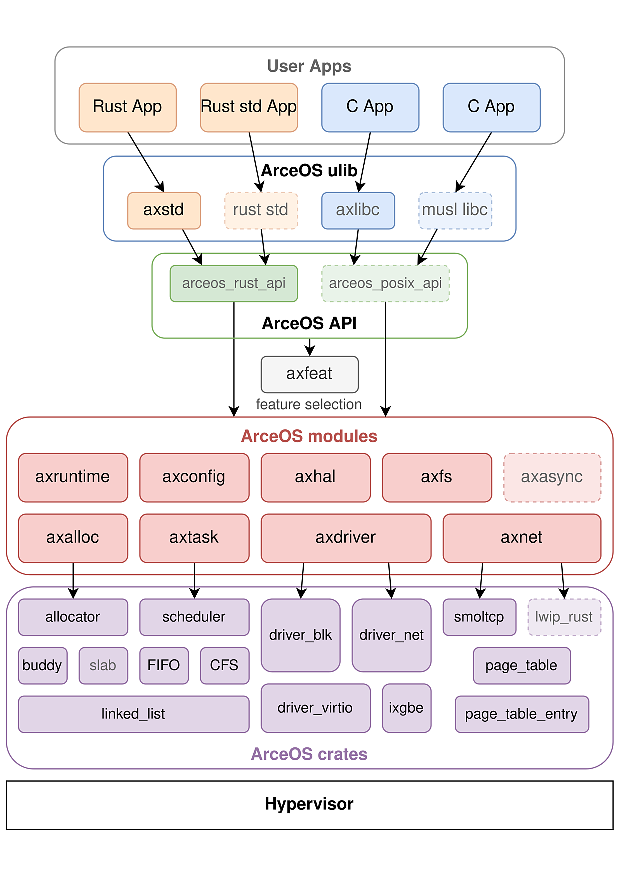
\includegraphics[width=0.5\linewidth]{ArceOS (1).pdf}
  \caption{ArceOS 内核结构图}
  \label{fig:ArceOS}
\end{figure}

每个模块包含多个组件,不同模块组合组合为应用程序提供底层支持。其中应用运行时模块
(axruntime)、硬件抽象层模块(axhal)以及动态内存分配模块(axalloc)是不可缺少的核心组件,
其他模块可以根据具体需求进行选择和使用。

在 ArceOS 的启动过程中,axhal 模块会将对应架构的 \_start 函数链接到 ".text.boot" 段, 作为 ArceOS 运行的第一段代码,完成一些基础的硬件相关初始化操作,例如设置栈指针、初始化页表和 MMU(内存管理单元)等,并跳转到 Rust 主函数 rust\_entry。
rust\_entry 函数位于 axruntime 模块中,它会依据不同的 Cargo 特性进行有针对性的初始化工作,若启用日志功能,会初始化日志系统;启用内存分配特性时,会查找物理内存区域并初始化全局内存分配器;接着会进行平台设备初始化,确保硬件正常工作。对于多任务、文件系统、网络、图形显示、对称多处理以及中断等特性,也会分别完成调度器、设备驱动、从 CPU、中断处理程序等的初始化。最后,它会调用应用的 main 函数,开启应用程序的执行,为操作系统和应用程序的运行构建起完整的基础环境。

当应用程序的 main 函数执行完毕后,若启用了 multitask (多任务)特性,将会调用 axtask::exit(0) 退出函数来退出当前任务;若未启用该特性,则会调用 axhal 模
块下的 misc::terminate 函数来结束整个系统的运行。

\section{ArceOS 内存管理组件及接口}
在 ArceOS 的模块中,axhal、axalloc、axmm 和 axdma 模块是 ArceOS 内存管理的核心模块,它们分别负责对不同硬件平台的硬件封装、物理内存分配、虚拟内存管理和直接内存访问,组成了如图~\ref{fig:ArceOS-mm} 所示的内存管理系统。

\begin{figure}
  \centering
  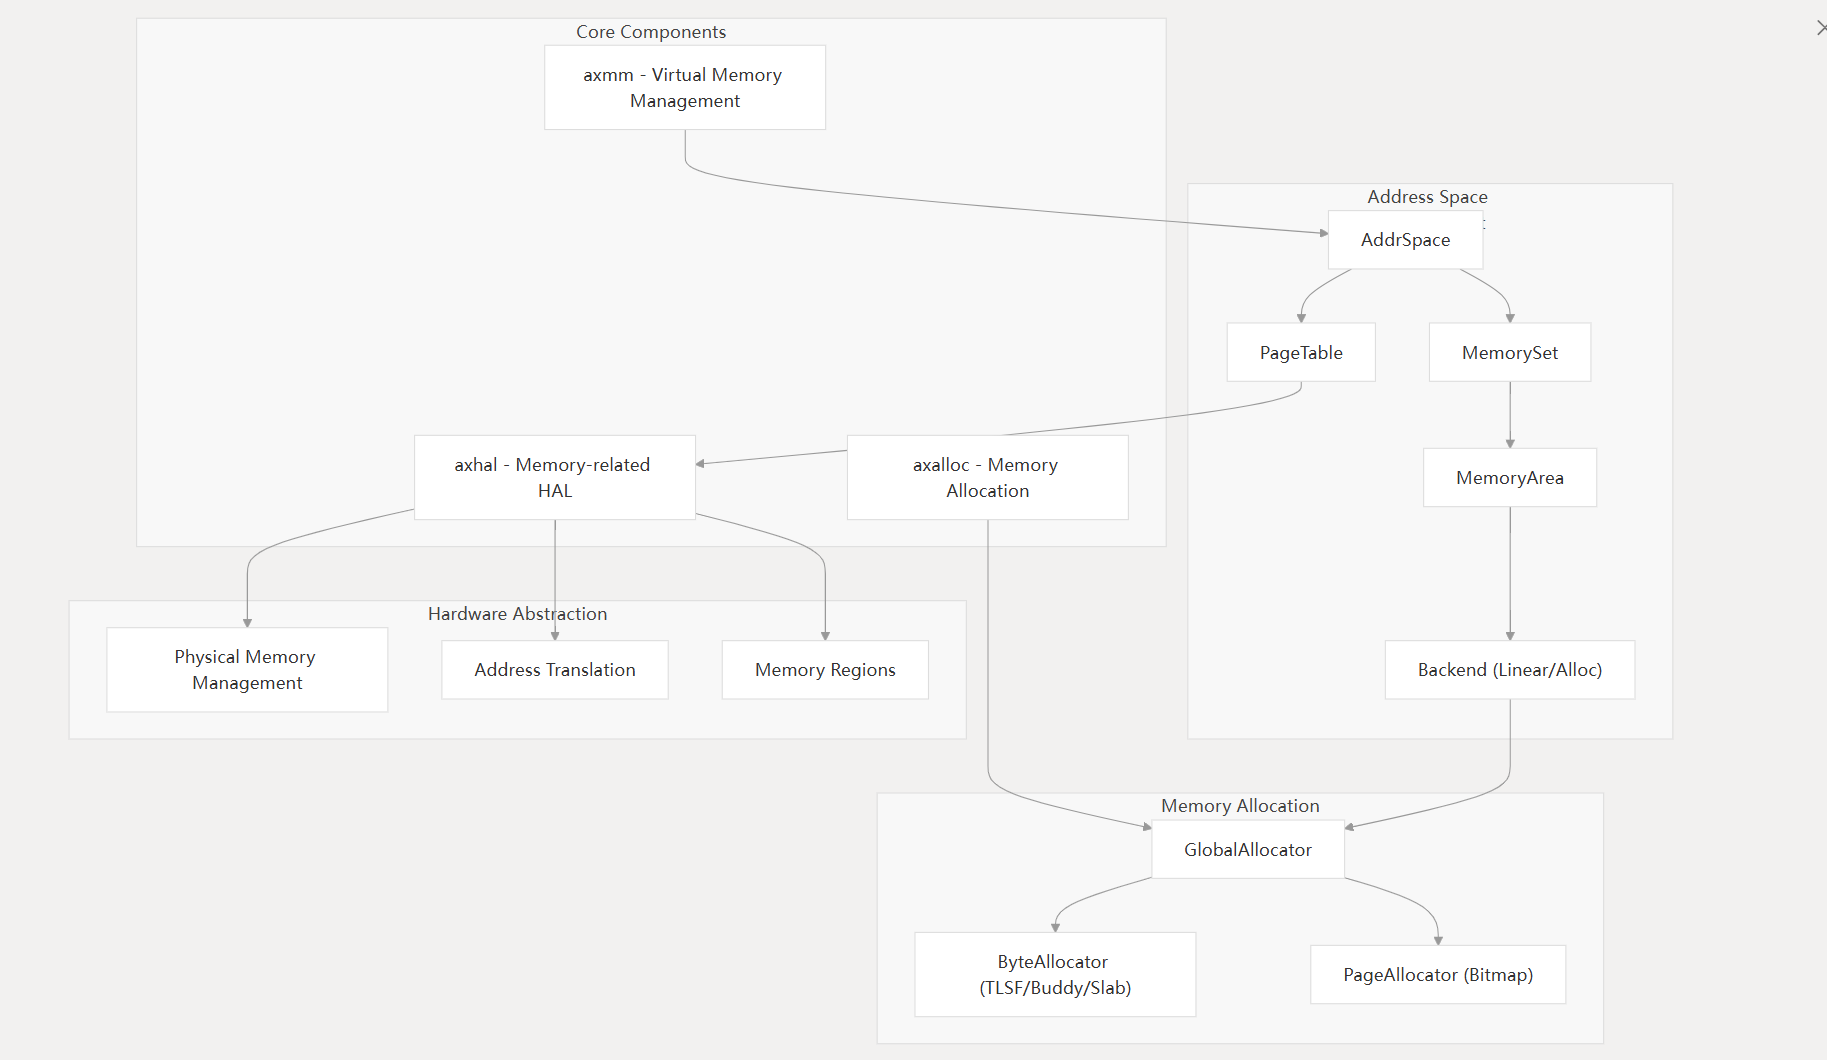
\includegraphics[width=1\linewidth]{arch.png}
  \caption{ArceOS 内存管理系统}
  \label{fig:ArceOS-mm}
\end{figure}

\subsection{axhal}

axhal 组件提供了一层针对不同硬件平台的硬件封装,它为指定的操作平台进行引导和初始化过程,并提供对硬件的操作。在内存方面,axhal 同样进行了一系列的封装操作来支持内存管理。例如:

\begin{itemize}
\item 页表管理封装:axhal 模块将不同架构的页表统一封装为 PageTable 类型,并提供了一致的操作接口,
例如 alloc\_frame(通过页表分配物理页帧)、dealloc\_frame(通过页表释放物理页帧)、phys\_to\_virt(将物理地址转换为虚拟地址)、set\_kernel\_page\_table\_root(设置内核页表根地址)和kernel\_page\_table\_root(获取内核页表根地址)等。
\item 内存区域封装:axhal 模块中定义了 MemRegion 结构体,用于表示和架构无关物理内存区域。MemRegion 结构体包含起始物理地址、区域大小、区域标志和区域名称等属性。通过该结构体,可以方便地管理和操作物理内存区域。
\item 获取内存区域的函数封装:axhal 提供 kernel\_image\_regions、default\_mmio\_regions、default\_free\_regions 接口用于获取内核映像区域、默认 MMIO 区域和默认空闲区域的内存区域列表,并将其封装为 MemRegion 类型。默认的 MMIO 区域和默认空闲区域的位置由 axconfig 模块定义,在不同的硬件平台上可能会有所不同。
\end{itemize}

\begin{figure}
  \centering
  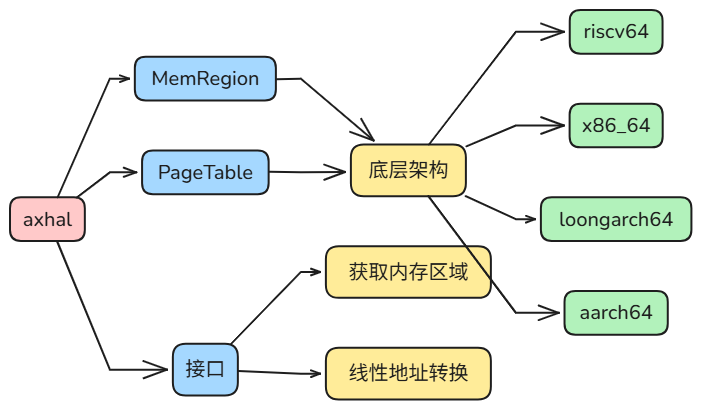
\includegraphics[width=1\linewidth]{axhal-arch.png}
  \caption{axhal 内存管理相关结构图}
  \label{fig:axhal-arch}
\end{figure}



\subsection{axalloc}

\begin{figure}
  \centering
  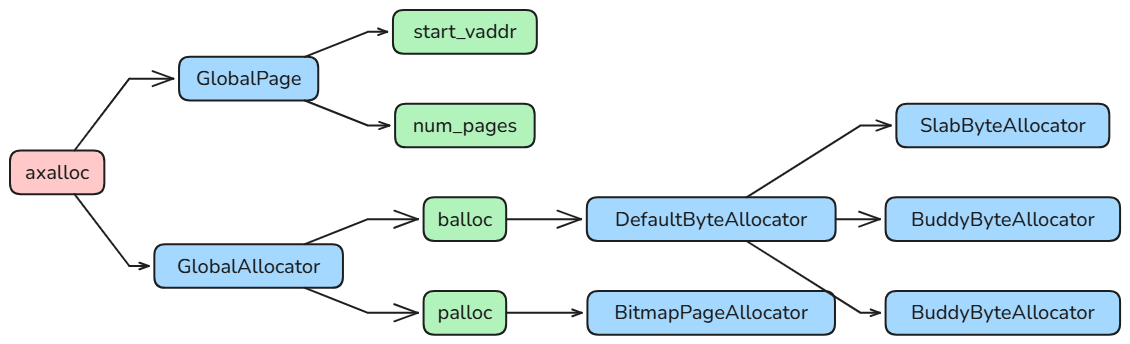
\includegraphics[width=1\linewidth]{axalloc-arch.png}
  \caption{axalloc 结构图}
  \label{fig:axalloc-arch}
\end{figure}

如图\ref{fig:axalloc-arch},axalloc 模块中定义了全局内存分配器 GlobalAllocator,由字节分配器和页面分配器组成。其中,字节分配器用于小内存块的分配和释放,在 ArceOS 中我们提供了三种不同的字节分配器:
\begin{itemize}
\item SlabByteAllocator——基于 slab 分配算法的字节分配器,其核心思想是将内存按照对象的大小进行分类,对于每一类对象,预先分配好一组连续的内存块,这些内存块组成一个 “slab”。每个 slab 包含了多个相同大小的对象槽(Object Slots),当需要分配某个特定大小的对象时,就从对应的 slab 中获取一个空闲的对象槽;当对象释放时,对应的对象槽又可以被重新利用。同时,为了更好地管理这些 slab,会有 slab 缓存(Slab Cache)机制,用于跟踪空闲和已使用的 slab 等状态。
slab 算法对于频繁分配和释放相同类型、相同大小对象的场景表现卓越,同类型对象集中存放使得在数据访问时对 CPU 缓存的利用更为充分,并且可以有效地减少内存碎片。但固定大小的 slab 可能会导致内存浪费和对于多样化、大小不一的内存分配需求适应性较差的问题。
\begin{figure}
  \centering
  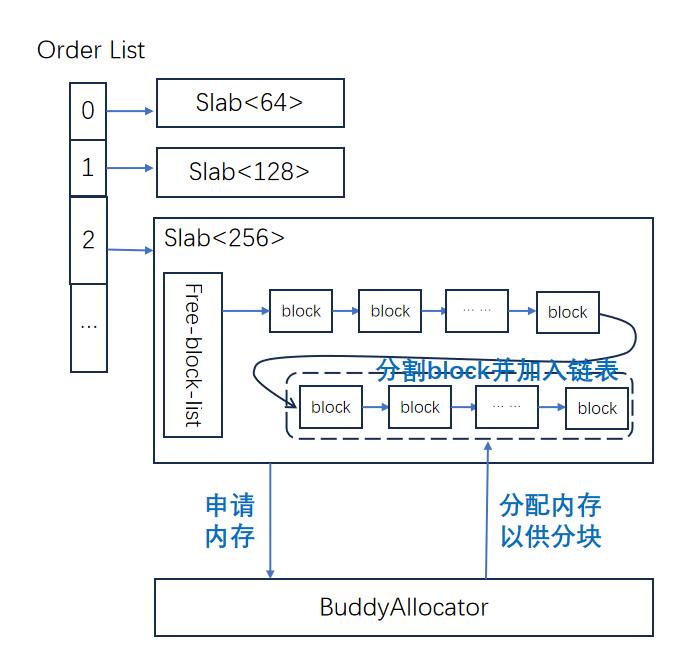
\includegraphics[width=0.7\linewidth]{Slab.png}
  \caption{Slab 算法示意图}
  \label{fig:Slab}
\end{figure}
\item BuddyByteAllocator——基于 Buddy 算法的字节分配器,以一种二叉树的思想来管理内存,它将整个内存空间看作是一个完整的、大小为 2 的幂次方的内存块,当需要分配内存时,如果有符合要求大小(同样是 2 的幂次方)的空闲内存块,就直接分配;若没有,则将更大的空闲内存块不断地二等分(即找到它的 “buddy”,也就是相邻且同样大小的另一半内存块),直到得到合适大小的内存块进行分配。在内存释放时,会检查释放的内存块与其 buddy 是否都空闲,如果是,则将它们合并成一个更大的空闲内存块,如此不断向上合并,直到不能合并为止。
Buddy 算法通过不断地合并空闲的 “伙伴” 内存块,能让内存空间保持相对规整,避免出现大量零散的小空闲块,内存释放时的合并操作判断和执行合并的过程也相对简单高效,但内存分配粒度受限于 2 的幂次方,可能会导致内存浪费和内部碎片问题。
\begin{figure}[H]
  \centering
  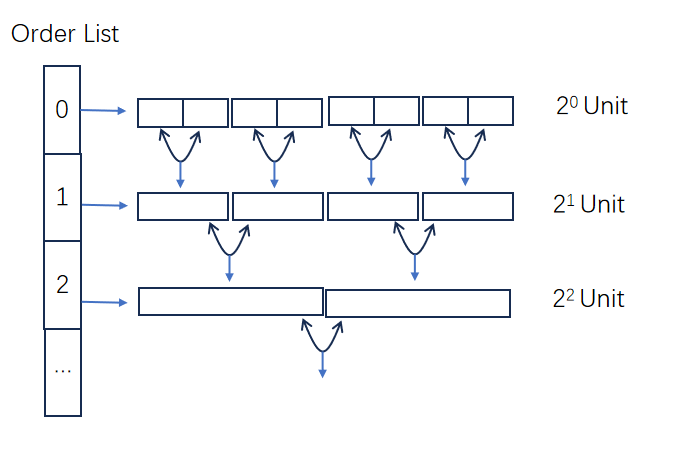
\includegraphics[width=0.7\linewidth,]{Buddy.png}
  \caption{Buddy 算法示意图}
  \label{fig:Buddy}
\end{figure}
\item TlsfByteAllocator——基于 TLSF(Two-Level Segregate Fit)算法的字节分配器,TLSF 采用了两级的分离适配结构。第一级是将整个内存空间按照不同大小范围划分成多个区间,每个区间对应着不同大小的内存块类别,形成一个区间链表。第二级则是针对每个区间,再使用一个位图(Bitmap)和一个空闲块链表来管理该区间内具体的空闲内存块。在进行内存分配时,先根据要分配的内存大小确定所属的区间,然后在位图中查找是否有合适的空闲块,若有则从对应的空闲块链表中取出进行分配;内存释放时,将释放的内存块重新插入到对应的空闲块链表,并相应更新位图信息。
TLSF 算法具有高效的分配速度和高内存利用率,可以灵活应对各种不同大小内存块的分配情况,但是维护两级结构中的各种管理信息使得内存开销相对较大。
\begin{figure}[H]
  \centering
  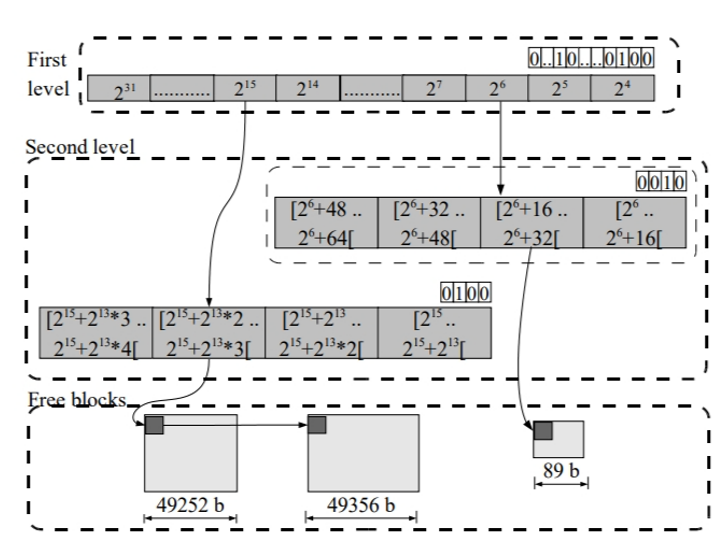
\includegraphics[width=0.7\linewidth]{TLSF.png}
  \caption{TLSF 算法示意图}
  \label{fig:TLSF}
\end{figure}
\end{itemize}

页分配器负责大型分配和扩展字节分配器,使用了标准库中的 BitmapPageAllocator,它是一个基于位图(bitmap)的页粒度内存分配器。它通过使用位图中的每一位来表示一个内存页的分配状态,从而实现高效的内存管理。该分配器支持不同大小的内存分配(从256MB到1TB),并且可以处理不同页大小(PAGE\_SIZE)的情况,要求页大小必须是2的幂次方。它提供了初始化内存区域、分配和释放内存页等基本功能,同时支持对齐分配和指定地址分配等特性。

全局内存分配器通过接口函数提供了对物理内存的操作功能,包括内存的分配、释放、查询等。其主要功能如下:
\begin{itemize}
\item 内存分配器类型选择:通过 Cargo 特性,axalloc 支持用户可以根据需求在 Buddy 分配器、Slab 分配器、TLSF 分配器中选择一种作为全局内存分配器的字节分配器部分。
\item 全局内存分配器初始化:axalloc 定义了一个静态全局变量 GLOBAL\_ALLOCATOR,
并实现了 core::alloc::GlobalAlloc 特性,将其注册为标准库的默认分配器。
在初始化时,需要调用global\_init函数,该函数会初始化页分配器和字节分配器。
\item 内存分配与释放:包括字节分配和释放、页面的分配和释放。
\item 内存状态查询:axalloc 提供了一些函数用于查询内存分配器的状态,如当前内存使用量、空闲内存量等。
\end{itemize}

另外,axalloc 模块提供了用于管理全局内存页面的类型 GlobalPage,其属性包括起始地址和包含的页数。并在全局内存分配器的支持下,提供分配单页和连续页面、填充页面等接口。同时,通过实现 Drop 特性,确保在 GlobalPage 被销毁时,自动释放其占用的内存。这种机制确保了内存资源的高效利用,避免了内存泄漏。

\subsection{axmm}

使用 axalloc 模块提供的内存管理功能,我们已经可以构建起一个简单的内存管理系统,支持内核和应用程序都处于同一地址空间,并且相互可见。
但是,在多任务或多进程的环境下,内核和应用程序之间的内存隔离是非常重要的。为了实现这一点,ArceOS 引入了 axmm 模块来实现虚拟内存管理,其结构如图所示。

\begin{figure}
  \centering
  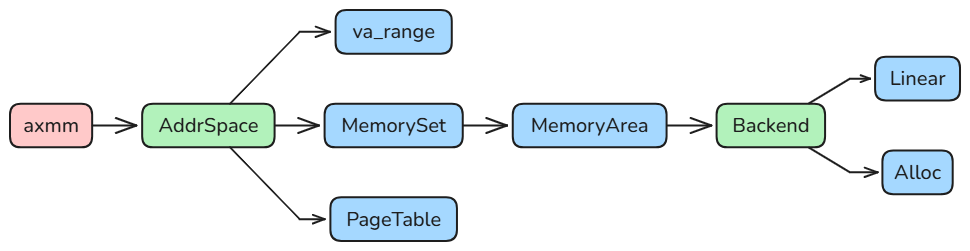
\includegraphics[width=1\linewidth]{axmm-arch.png}
  \caption{axmm 结构图}
  \label{fig:axmm-arch}
\end{figure}


axmm 模块的核心是 AddrSpace 结构体,它表示一个虚拟内存地址空间,包含虚拟地址范围、内存区域集合以及页表。通过该结构体提供的接口,可以对虚拟内存地址空间进行管理,包括创建、映射、解除映射、读写数据等操作。
AddrSpace 的具体接口如图\ref{fig:AddrSpace}所示:
\begin{figure}
    \centering
    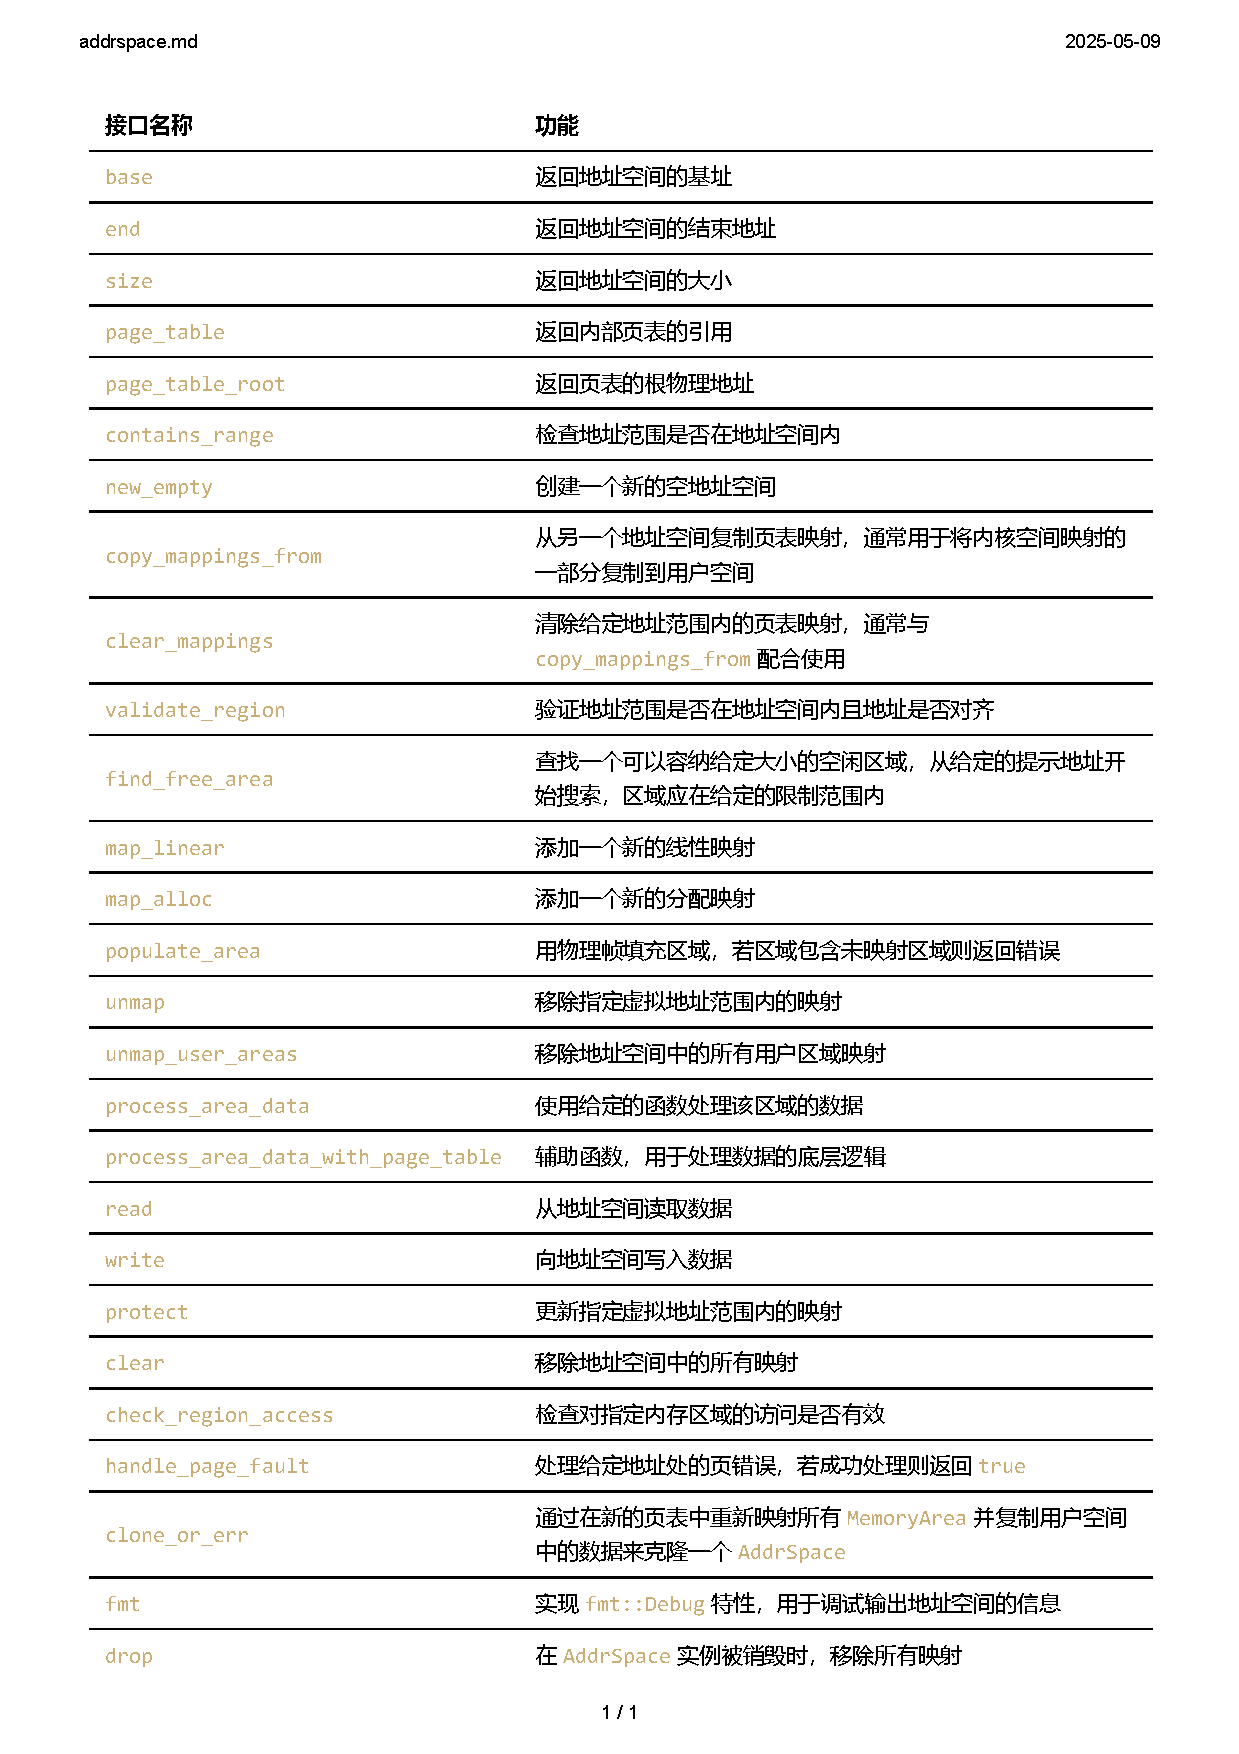
\includegraphics[width=1\linewidth]{addrspace.pdf}
    \caption{AddrSpace 结构体接口}
    \label{fig:AddrSpace}
\end{figure}

实现 AddrSpace 结构体及其接口对于构建一个高效、灵活且安全的虚拟内存管理系统具有极其重要的意义。一方面,通过为每个进程分配独立的虚拟地址空间,AddrSpace 不仅实现了内核与用户空间的隔离,还确保了进程之间的相互独立,从而防止了进程间的非法访问和潜在的破坏行为。

另一方面,AddrSpace 提供的内存保护机制进一步增强了系统的安全性。它通过页表和访问权限控制,确保每个进程只能访问自己被授权的内存区域,同时在检测到非法访问时能够及时触发异常并进行处理,从而避免系统崩溃。这种机制不仅保护了内核的稳定性,还为用户程序提供了可靠的运行环境。

除 AddrSpace 结构体及其接口外,axmm 模块还定义 Backend 核心抽象,用于处理不同类型的内存映射实现细节。它作为 MemoryArea (内存区域)的后端,将虚拟地址与物理存储关联起来,将映射、解除映射、处理页面异常等操作传递到具体的后端实现,进而完成对页表的操作。axmm 模块支持两种类型的内存映射后端:
\begin{itemize}
\item Linear Backend:用于与已知物理地址的直接映射,例如内存映射的 I/O 区域或内核映像部分,虚拟地址和物理地址具有固定的偏移关系;
\item Allocation Backend:按需分配物理页,支持延迟分配,常用于用户空间内存管理。
\end{itemize}

内存区域对应的映射类型在内存区域对象创建时,即调用 AddrSpace 的 map\_linear 或 map\_alloc 方法申请空间并进行映射时指定。

\subsection{axdma}
axdma 模块实现了 DMA 内存管理,提供了直接内存访问的接口。DMA(Direct Memory Access,直接内存访问) 是一种硬件特性,允许某些硬件子系统在不经过 CPU 控制的情况下直接访问系统内存,
DMA 通常用于高速数据传输,例如从硬盘读取数据到内存,或者从内存将数据发送到网络接口。

在传统的数据传输中,CPU 需要逐字节地从外设读取数据,然后将其写入内存,或者从内存读取数据后写入外设。这种操作不仅效率低下,还会占用大量的 CPU 时间。而 DMA 允许外设直接访问内存,
无需 CPU 参与,从而提高了数据传输的速度和效率,并释放了 CPU 的计算资源,使其可以处理其他任务。

\begin{figure}[H]
    \centering
    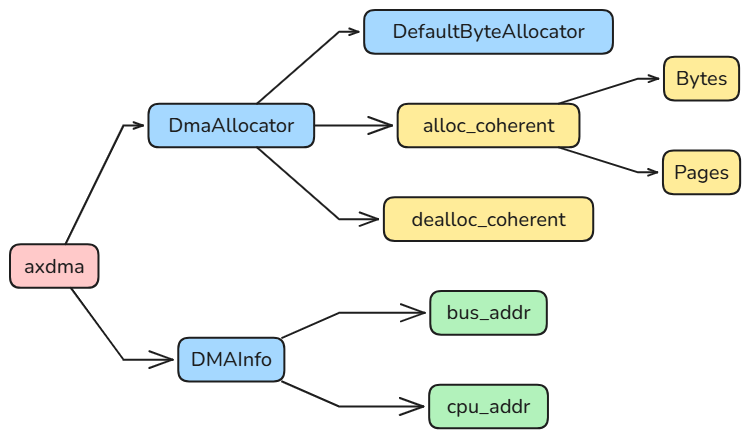
\includegraphics[width=1\linewidth]{axdma-arch.png}
    \caption{axdma 结构图}
    \label{fig:axdma-arch}
\end{figure}

如图\ref{fig:axdma-arch},ArceOS 的 DMA 模块通过实现 DMA 分配器(DmaAllocator),向设备驱动模块(axdriver)提供了 DMA 内存分配和释放的接口。
它会根据设备的需求,分配合适大小的内存块,并在 DMA 操作完成后释放这些内存块。
DMA 分配器还会处理 DMA 操作中的地址转换问题,将虚拟地址转换为总线地址,以便于 CPU 访问。
DMAInfo 结构体则记录了用于 DMA 操作的内存区域相关的信息,包括 CPU 访问该区域的虚拟地址和该区域在总线上的物理地址。
同时,DMA 分配器分配的内存需要标记为 UNCACHED,以避免缓存一致性问题,这需要虚拟内存管理模块(axmm)提供的接口来完成。

DMA 模块的具体接口如图\ref{fig:DmaAllocator}所示:
\begin{figure}[H]
    \centering
    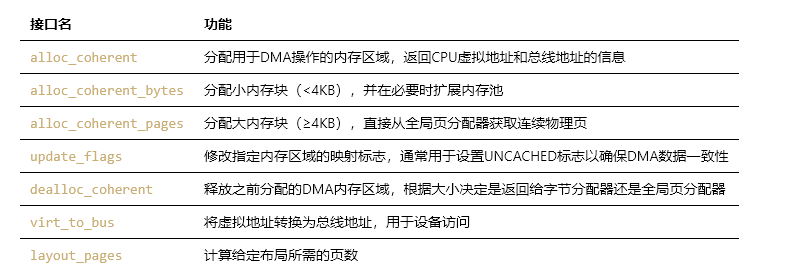
\includegraphics[width=0.7\linewidth]{axdma.png}
    \caption{DmaAllocator 结构体接口}
    \label{fig:DmaAllocator}
\end{figure}

\section{ArceOS 内存管理机制}

% ArceOS 中与内存管理相关的结构主要有:

% \begin{itemize}
% \item MemRegion:表示一个物理内存区域,包含起始物理地址、区域大小、区域标志和区域名称。
% \item GlobalAllocator:全局内存分配器,用于管理物理内存区域,包含用于小分配的字节分配器和用于大型分配和扩展字节分配器的页分配器,提供了内存和页面的分配和释放接口。
% \item AddrSpace:表示虚拟内存地址空间,包含虚拟地址范围、内存区域集合以及页表。通过该结构体提供的接口,可以对虚拟内存地址空间进行管理,包括创建、映射、解除映射、读写数据等操作。
% \item MemoryArea:表示一块虚拟内存区域,包含起始地址、结束地址、访问权限和映射关系等信息。
% \item MemorySet:表示虚拟内存区域的集合构成的 Btree 结构,提供管理虚拟内存区域的具体方法。
% \item Backend:内存映射后端,包括 Linear Backend 和 Allocation Backend。
% \end{itemize}

在本章第一节中我们提到了 ArceOS 的启动和初始化过程,而在这里我们将对其中与内存分页相关的部分进行详细分析:
架构的初始化函数 \_start 中进行了启动页表和内存管理单元的初始化,为 QEMU 虚拟机的物理内存等关键区域构建映射,设置根页表地址并刷新 TLB,完成分页的早期启动阶段。
这一阶段是 ArceOS 默认开启的,构建的映射为恒等映射,虚拟地址和物理地址相同,主要用于内核的启动和初始化。
\begin{lstlisting}[language=c, caption=\_start]
phys_virt_offset = const PHYS_VIRT_OFFSET,
boot_stack_size = const TASK_STACK_SIZE,
boot_stack = sym BOOT_STACK,
init_boot_page_table = sym init_boot_page_table,
init_mmu = sym init_mmu,
\end{lstlisting}

如图~\ref{fig:init}所示,分页的早期启动阶段完成后,如果开启了 paging 特性,在 rust\_main 函数中会调用 axmm 模块的 init\_memory\_management 函数初始化内存管理,
即创建内核的虚拟地址空间,为内核的虚拟地址空间构建线性映射,调用 axhal 的接口设置内核的虚拟地址空间的页表,并将其设置为当前的页表根,完成分页的重建映射阶段。
该阶段将内核和用户空间的虚拟地址空间隔离开来,让内存管理模块能够管理更大的地址空间,为 DMA 和多任务等功能提供支持。

\begin{figure}[H]
    \centering
    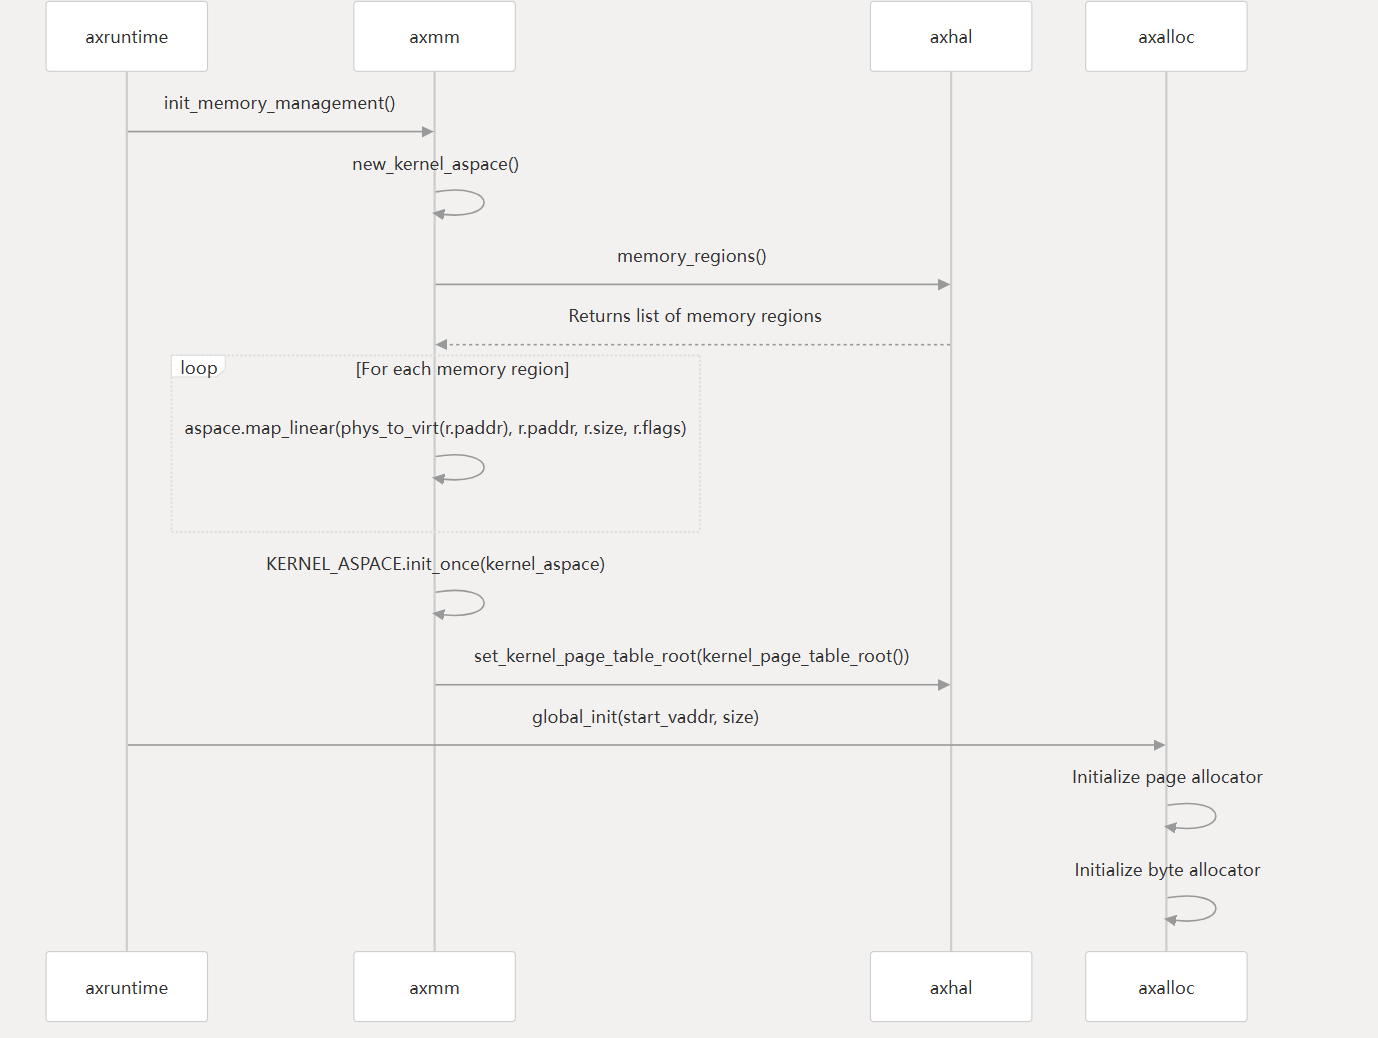
\includegraphics[width=1\linewidth]{init.png}
    \caption{分页的重建映射阶段}
    \label{fig:init}
\end{figure}

开启 paging 特性且上层架构或者应用需要对内存空间进行操作时,会调用 AddrSpace 的相应接口,如 find\_free\_area(寻找空闲内存区域)、map\_linear(建立线性映射)、map\_page(建立分配映射)等方法,这些方法会根据具体的内存操作需求,对页表和虚拟地址空间进行操作,并调用全局内存分配器进行物理内存的分配和释放。全局分配器在分配时会先尝试从字节分配器分配,如果字节分配器内存不足,则计算需要多少内存,从页面分配器分配页面后将页面添加到字节分配器重新进行分配,此方法允许高效处理小型和大型分配,同时保持合理的内存使用率。

同时,ArceOS 还在 AddrSpace 结构体中提供了页面异常的处理接口,例如当访问的虚拟地址对应的物理页不存在时,会触发缺页异常,此时会调用 AddrSpace 的 handle\_page\_fault 函数处理缺页异常,
该函数会对后端为 Alloc 类型的地址,调用 axalloc 中的全局内存分配器进行物理页的分配,并通知 axhal 中的页表更新映射关系。对于后端为 Linear 类型或者需要填充的地址,则会处理失败,返回 false,
因为这两类的地址在创建时就应完成物理页的分配和映射,缺页异常的处理不适用。AddrSpace 的 handle\_page\_fault 函数的流程图如图~\ref{fig:handle-page-fault-arceos}所示:

\begin{figure}[H]
    \centering
    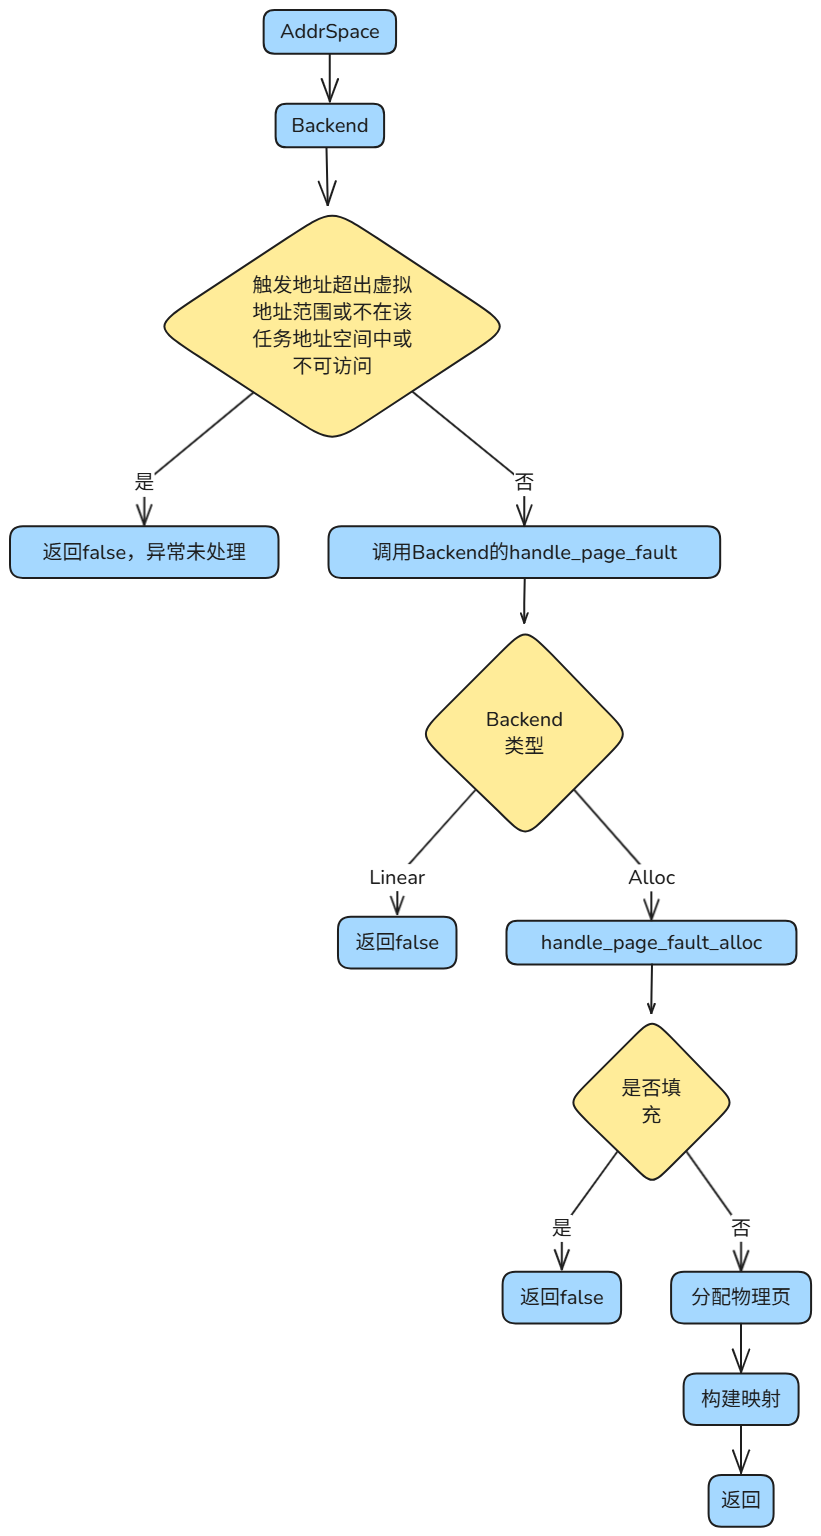
\includegraphics[width=0.7\linewidth]{pagefault-arceos.png}
    \caption{handle\_page\_fault 函数流程图}
    \label{fig:handle-page-fault-arceos}
\end{figure}


借助缺页异常的处理,ArceOS 还实现了 Lazy Map 机制,即当访问的虚拟地址对应的物理页不存在时,不会立即分配物理页,而是在第一次访问该虚拟地址时才触发缺页异常,进行分配和映射。
% !TeX root = ../cyh.tex

\chapter{starry-next 宏内核}

\section{starry-next 宏内核整体架构}

Starry-next (StarryOS) 是构建在 ArceOS 基础之上的操作系统内核。它实现了一个兼容 Linux 的系统调用接口,同时支持多种硬件架构,包括 x86\_64、riscv64、aarch64 和 loongarch64。

代码结构上,Starry-next 主要由以下模块组成:

\begin{itemize}
\item core:基于 ArceOS 的底层支持实现 StarryOS 的核心内核功能,包括内存管理(mm)、任务管理(task)和时间管理(time)等。其中内存管理模块负责分配、释放和映射,如 copy\_from\_kernel 函数用于将内核空间的映射复制到用户地址空间,load\_user\_app 函数用于加载用户应用程序到内存中。任务管理模块处理任务和线程的创建、调度和管理,例如 new\_user\_task 函数用于创建新的用户任务。时间管理模块管理系统时间和定时器。
\item api: 现面向用户的 API 和系统调用接口,涵盖文件系统操作、进程管理、线程管理、内存管理等多个方面。
\item src:主要负责启动主函数、加载应用程序并对系统调用的分发进行处理。
\item 其他:包括用于适配不同架构的配置文件和工具链,以及用于构建和运行 StarryOS 的构建工具和脚本。
\end{itemize}

功能上,Starry-next 也可以划分为较为独立的模块:

\begin{itemize}
\item 内存管理模块:负责管理物理内存和虚拟内存,包括内存分配、映射和释放等操作。
\item 进程管理模块:负责管理进程和线程,包括进程创建、调度和管理等操作。
\item 文件系统模块:负责管理文件系统,包括文件的创建、读取、写入和删除等操作。
\item 网络模块:负责管理网络操作,包括网络协议栈、网络设备驱动等操作。
\item 系统信息模块:负责提供系统信息和状态,包括 CPU、内存、网络等信息。
\item 信号模块:负责处理信号和中断,包括信号的发送、接收和处理等操作。
\end{itemize}

每个功能模块都需要向应用程序提供相应的系统调用接口,为应用程序提供内核服务。同时,功能模块还需要尽可能复用 ArceOS 的底层组件和接口,以减少代码的重复和维护成本。
功能模块之间通过明确定义的接口进行通信,确保系统的稳定性和可拓展性。

通过结构和功能上的划分与解耦,Starry-next 宏内核的每个模块都可以独立开发、测试和维护,增强了系统的可拓展性和稳定性,也使得本课题大方向上的多名开发者可以在同一代码库上进行协作开发。

\begin{figure}[H]
    \centering
    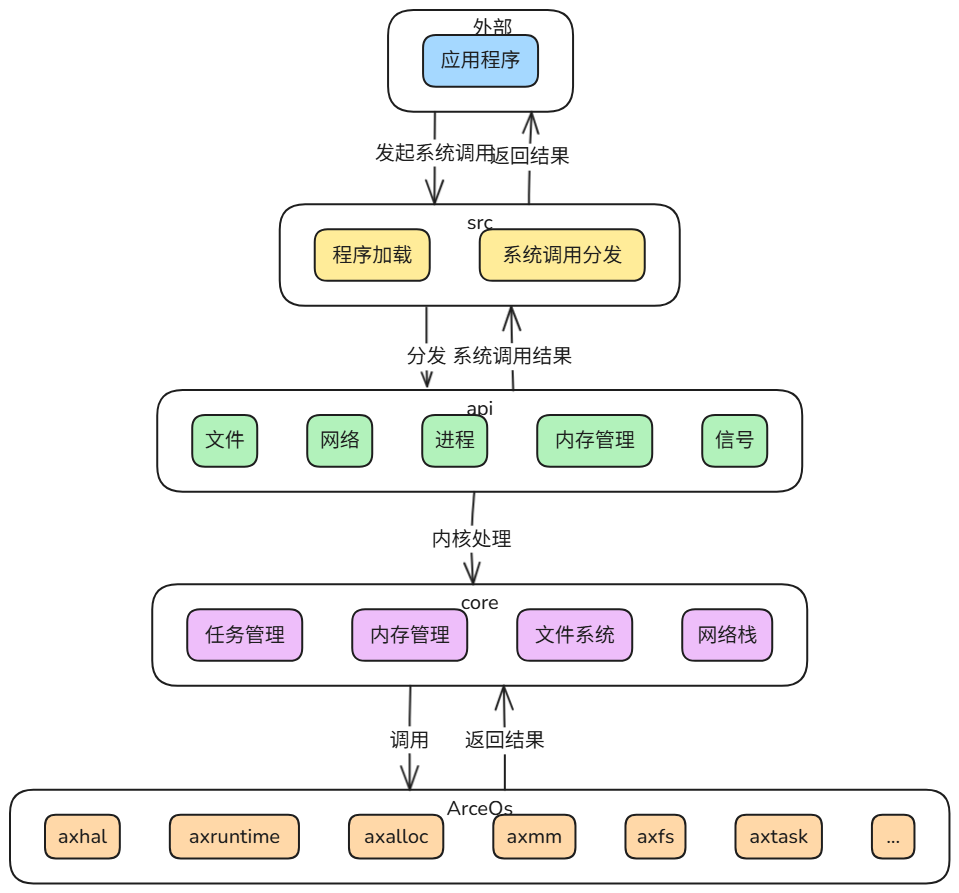
\includegraphics[width=0.7\linewidth, keepaspectratio]{starry-arch.png}
    \caption{starry-next 宏内核架构}
    \label{fig:starry-next}
\end{figure}

\section{starry-next 初始化和运行过程}

% Starry-next 以 main 函数作为系统的入口点,创建初始化进程,为环境变量指定的测试用例创建用户应用程序,并依次运行这些应用程序。在运行过程中,Starry-next 会根据系统资源的需求,动态地分配和管理内存,同时处理各种系统调用,如 fork、exec、wait、mmap、munmap 等。

starry-next 的初始化从 Bootloader 将控制权交给内核入口点开始,之后 ArceOS 的 axhal 模块和 axruntime 模块会完成硬件的初始化,并根据选择的特性进行内存管理器、任务管理器、文件系统、网络等模块的初始化。接着,axruntime 模块以 src 中 main 函数创建一个初始化进程,进而为环境变量指定的测试用例创建用户应用程序,并将用户程序加载到内存中。

% 在运行过程中,starry-next 会根据系统资源的需求,动态地分配和管理内存,同时处理各种系统调用,如 fork、exec、wait、mmap、munmap 等。这些系统调用会使操作系统内核进入内核态,执行 core 中相应的处理程序,并调用底层的 ArceOS 提供的接口进行处理。
% 最后的处理结果将返回系统调用层,进而返回给用户空间的应用程序。

在运行过程中,starry-next 会逐个运行应用程序,并根据系统资源的需求,动态地分配和管理内存。
当应用程序发起系统调用时,先由 src 层将参数根据系系统调用号分发到 api 层的相应处理函数,
api 层的函数会检查参数的类型、取值范围等是否符合系统调用的规范。验证参数无误后,api 层函数会根据系统调用的具体功能,调用 core 层的相关功能模块及其底层的 ArceOS 组件来完成实际的操作。
当 core 层完成操作并返回结果后,api 层会对返回结果进行处理。如果操作成功,api 层会将结果按照系统调用的约定进行封装,以便返回给应用程序。如果操作失败,api 层会根据错误类型设置合适的错误码。
最后,api 层的函数会将处理结果返回给 src 层,src 层会将结果返回给应用程序。

\begin{figure}[H]
    \centering
    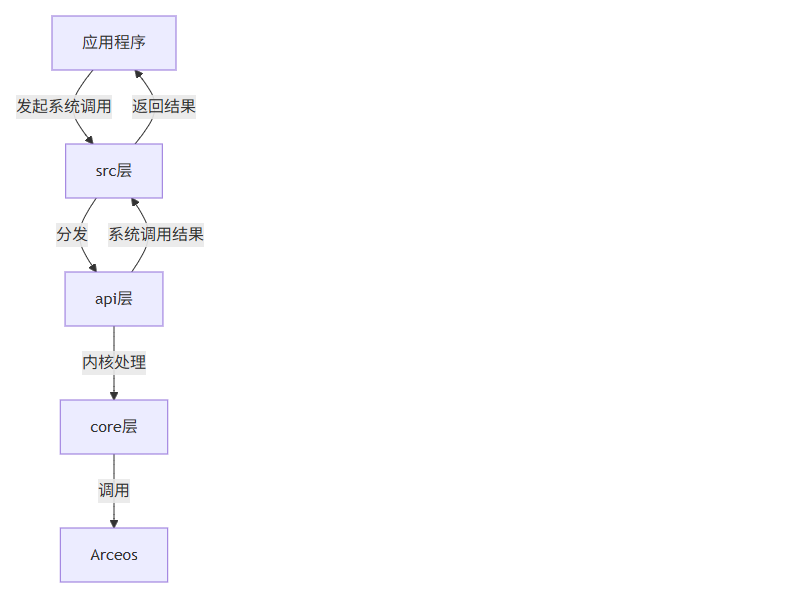
\includegraphics[width=1\linewidth, keepaspectratio]{syscall.png}
    \caption{系统调用流程}
    \label{fig:syscall}
\end{figure}


\section{starry-next 内存管理模块}

\subsection{模块结构}

\begin{figure}[H]
    \centering
    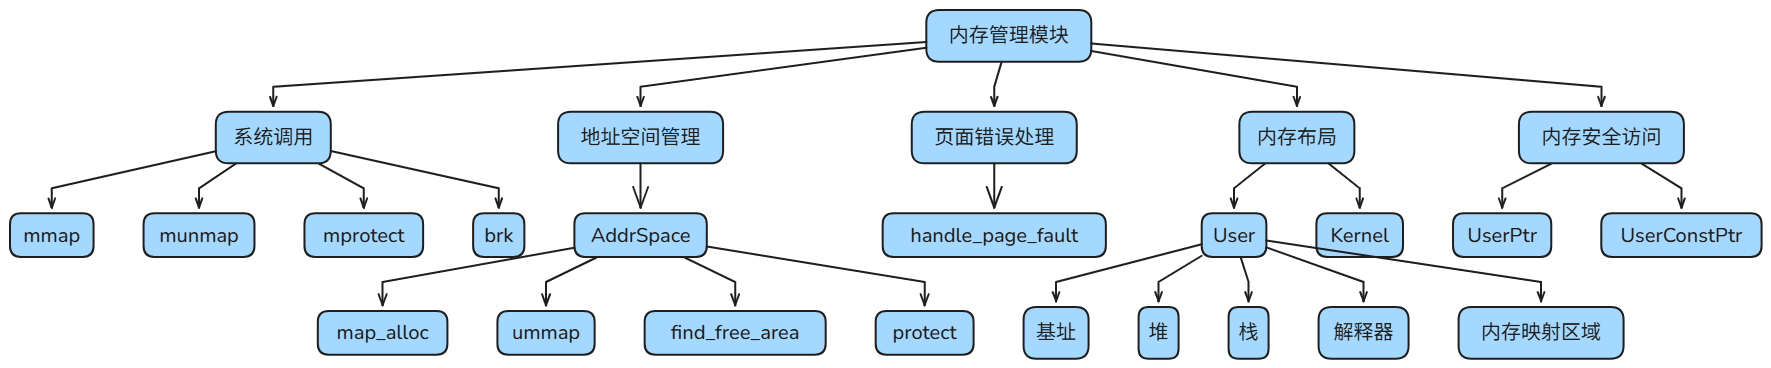
\includegraphics[width=1\linewidth, keepaspectratio]{mm-arch2.png}
    \caption{starry-next 内存管理模块结构}
    \label{fig:mm-arch}
\end{figure}

starry-next 的内存管理模块主要由以下部分组成:

\begin{itemize}
    \item 系统调用:提供了一系列系统调用接口,用于管理内存,如 mmap、munmap、mprotect、brk 等。
    \item 地址空间管理:使用 AddrSpace 结构体及其接口管理用户程序的地址空间,包括内存映射、权限控制等。
    \item 页面异常处理:当用户程序访问内存空间时触发的缺页异常会调用相应的处理函数。
    \item 内存布局:定义了内存布局,包括内核空间和用户空间的划分。
    \item 安全内存访问:通过指针封装提供对用户空间内存的安全访问。
\end{itemize}

\subsection{内存管理机制}

starry-next 的内存管理基本上复用了 ArceOS 的内存管理机制:使用 ArceOS 提供的 AddrSpace 结构体管理用户程序的内存空间,当用户程序需要对内存进行操作时,会调用相应的系统调用,如 mmap、munmap、mprotect、mremap 等,这些系统调用会调用 AddrSpace 结构体的接口在用户地址空间中创建和管理内存映射,同时也会调用全局内存分配器进行物理页的分配和映射。

但作为宏内核,starry-next 需要区分内核态和用户态,因此还对内存管理进行了进一步的优化和扩展,例如为用户态和内核态分别设置了不同的地址空间,并且用户态进程不能直接访问内核态内存空间,
而是需要发出系统调用,通过 trap 机制进入内核态,再进行对应处理,通过这种方式来实现用户态和内核态的隔离;在一些架构中将内核部分的映射复制到用户地址空间,使用户态进程可以直接访问内核的某些数据结构或代码片段,
可以减少内核态和用户态之间的切换开销,提高系统的性能。

\subsection{页面异常处理}
页面异常的处理方面,starry-next 在 ArceOS 的基础上增加了判断:如果是用户态程序访问内存空间或者是内核态程序访问用户内存空间时触发的缺页异常,才会调用用户程序的 handle\_page\_fault 函数,
也就是 ArceOS 的 AddrSpace 结构体提供的页面错误处理函数处理缺页异常,该函数会根据虚拟地址的映射关系,调用全局内存分配器进行物理页的分配和映射。
如果 AddrSpace 结构体不能成功处理该异常,则会打印错误信息并终止当前任务,并发送 SIGSEGV 信号。

\begin{figure}[H]
    \centering
    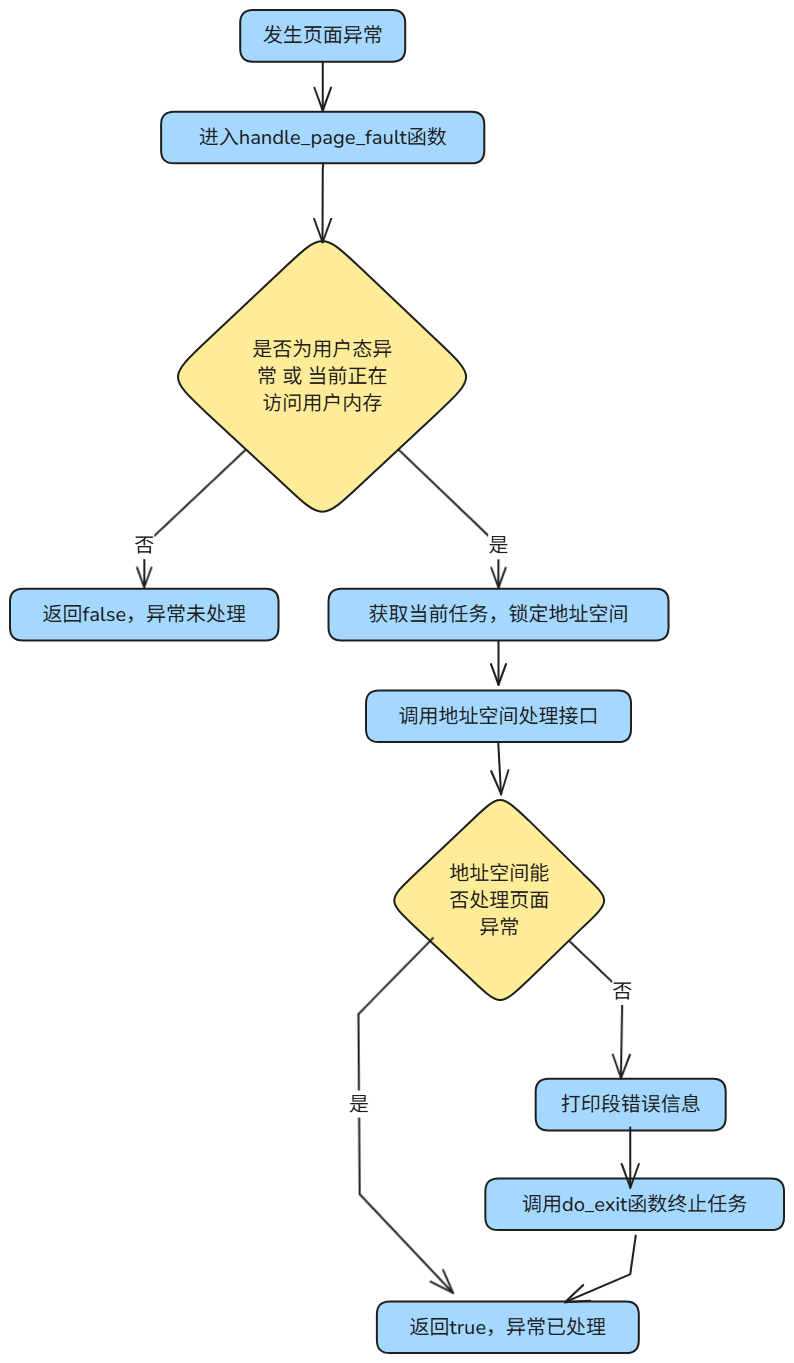
\includegraphics[width=0.7\linewidth, height=14cm,keepaspectratio]{pagefault-starry.png}
    \caption{starry-next 页异常处理}
    \label{fig:pagefault-starry}
\end{figure}

\subsection{内存布局}

不启动 ArceOs 的 paging 特性时,应用和内核在同一空间中运行,系统直接使用物理地址。物理空间的结构如图\ref{fig:phy-layout2}所示。
在 Cargo 项目启动时,axhal 组件的 build.rs 构建文件会根据根据 linker.lds.S 文件中的链接脚本,将物理空间划分为多个部分——内核部分从指定的基地址开始,首先放置可执行代码段(.text),然后是只读数据段(.rodata)和初始化函数数组(.init\_array)。接着是可读写数据段(.data),线程局部存储相关段(.tdata 和 .tbss),以及每个CPU核心的私有数据段(.percpu)。最后是未初始化数据段(.bss),其中包含了启动栈空间,设备内存则位于 0 地址和内核空间之间。整个布局严格遵循4K对齐,并在最后定义了一些与中断处理、系统调用等相关的自定义段。

\begin{figure}[H]
\centering %图片全局居中
%并排几个图,就要写几个minipage
\begin{minipage}[b]{0.45\textwidth} %所有minipage宽度之和要小于1,否则会自动变成竖排
\centering %图片局部居中
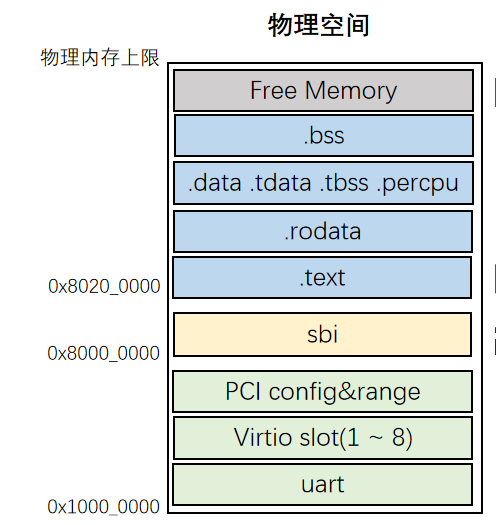
\includegraphics[width=0.8\textwidth]{phy-layout.png} %此时的图片宽度比例是相对于这个minipage的,不是全局
\caption{物理内存布局}
\label{fig:phy-layout2}
\end{minipage}
\begin{minipage}[b]{0.45\textwidth} %所有minipage宽度之和要小于1,否则会自动变成竖排
\centering %图片局部居中
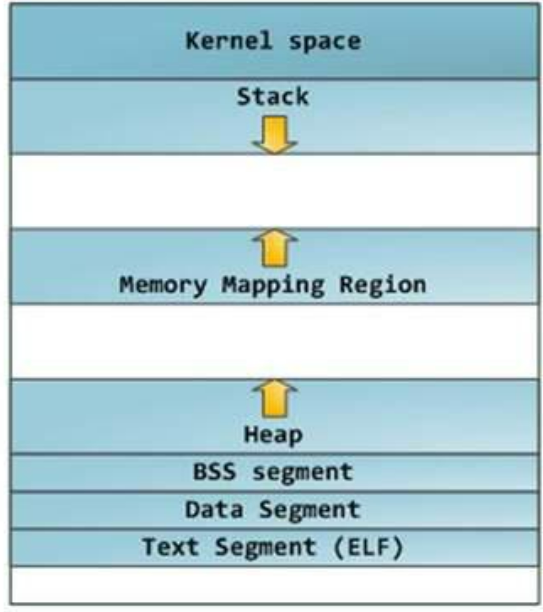
\includegraphics[width=0.8\textwidth]{virt-layout.png}%此时的图片宽度比例是相对于这个minipage的,不是全局
\caption{进程虚拟空间布局}
\label{fig:virt-layout2}
\end{minipage}
\end{figure}


% \begin{figure}[H]
%     \centering
%     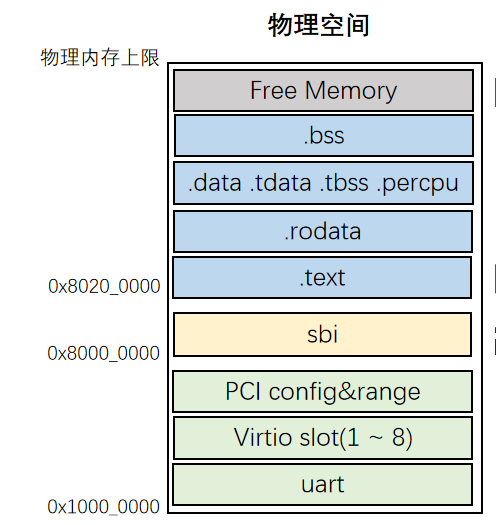
\includegraphics[width=0.5\linewidth, keepaspectratio]{phy-layout.png}
%     \caption{物理内存布局}
%     \label{fig:phy-layout}
% \end{figure}

starry-next 启动了 paging 特性,为每个应用程序分配一个独立的的虚拟地址空间,即 AddrSpace 结构体,用于管理用户程序的内存空间。如图\ref{fig:virt-layout2}所示,进程地址空间分为用户空间和内核空间两部分,用户空间位于低地址,包括了代码段、数据段、堆、栈、内存映射区域。
其中,代码段和数据段是用户程序的只读和读写数据,堆是用户程序的动态内存分配区域,栈是用户程序的函数调用和局部变量存储区域。
内核空间位于高地址,包括了内核代码段、内核数据段、内核堆、内核栈、页表。不同架构下各部分的具体起始地址和大小会有所不同,具体设置可参照表\ref{tab:virt-layout-config}。
% \begin{figure}[H]
%     \centering
%     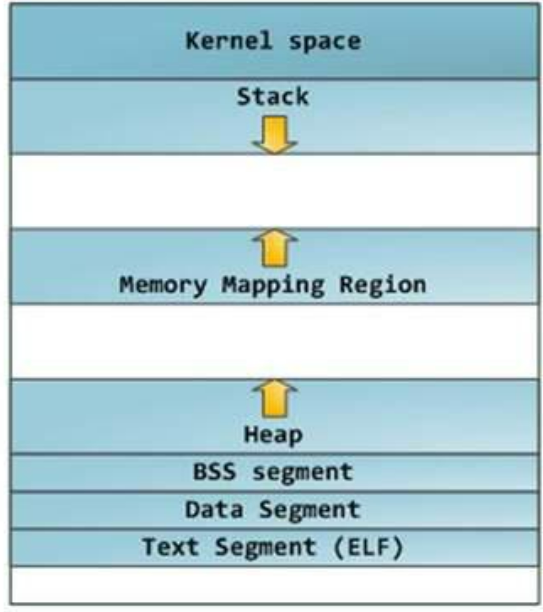
\includegraphics[width=0.5\linewidth, keepaspectratio]{virt-layout.png}
%     \caption{进程虚拟空间布局}
%     \label{fig:virt-layout}
% \end{figure}

\begin{table}[!ht]
    \centering
    \begin{tabular}{lllll}
    \hline
        ~ & x86\_64 & RISC-V 64 & AArch64 & LoongArch64  \\ \hline
        User space base & 0x1000 & 0x1000 & 0x1000 & 0x1000  \\ \hline
        User space size & 128 TB & 4 GB & 128 TB & 4 GB  \\ \hline
        User interpreter base & 64 MB & 64 MB & 64 MB & 64 MB  \\ \hline
        User heap base & 1 GB & 1 GB & 1 GB & 1 GB  \\ \hline
        User heap initial size & 64 KB & 64 KB & 64 KB & 64 KB  \\ \hline
        User stack top & 0x7fff\_0000\_0000 & 0x4\_0000\_0000 & 0x7fff\_0000\_0000 & 0x4\_0000\_0000  \\ \hline
        User stack size & 64 KB & 64 KB & 64 KB & 64 KB  \\ \hline
        Kernel stack size & 256 KB & 256 KB & 256 KB & 256 KB \\ \hline
    \end{tabular}
    \caption{各架构虚拟空间设置}
    \label{tab:virt-layout-config}
\end{table}

\subsection{安全内存访问}

为了保证系统的安全性和稳定性,starry-next 对用户空间内存的访问进行了严格的控制和保护,通过指针封装提供对用户空间内存的安全访问。
具体来说,starry-next 定义了 UserPtr 和 UserConstPtr 两个安全指针类型,分别表示指向用户空间内存的可变和不可变指针。
在访问用户空间内存时,要检查地址是否对齐、当前任务是否有权限访问该地址、地址是否在用户空间范围内并于已经分配映射。
如果这些条件都满足,则可以安全地访问用户空间内存,否则会抛出异常并终止当前任务。

UserPtr 和 UserConstPtr 提供了一系列接口,用于对用户空间内存进行访问和修改。例如:
负责基本信息的查询的 address(获取指针所指向的虚拟地址)和 is\_null(判断指针是否为空)和
获取切片和引用的 get\_as\_mut 和 get\_as\_mut\_slice 等。

\begin{figure}[H]
    \centering
    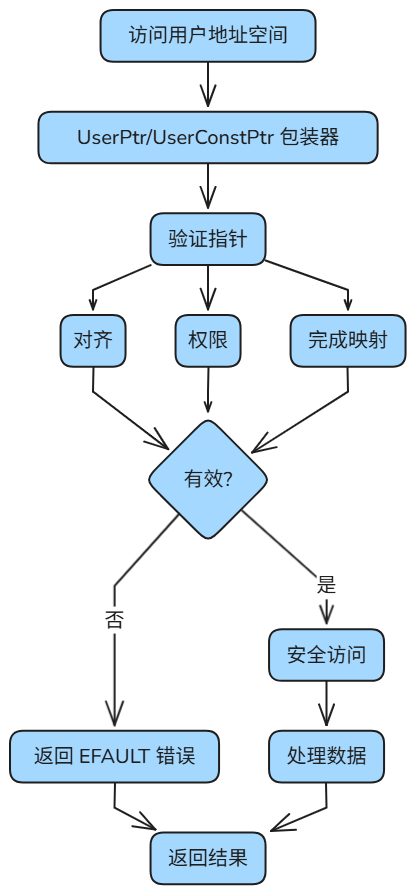
\includegraphics[width=0.5\linewidth]{ptr.png}
    \caption{安全内存访问流程}
    \label{fig:ptr}
\end{figure}
% !TeX root = ../cyh.tex


\chapter{内存管理子系统接口的设计与实现}

\section{内存管理子系统概述}

前两章中我们分别介绍了 ArceOS 基座中的内存管理组件和 starry-next 的内存管理模块,
而本小节则将二者串联起来,从 crate (即 Rust 模块,本节简称为模块)层面介绍内存管理子系统的结构。

\begin{figure}[H]
    \centering
    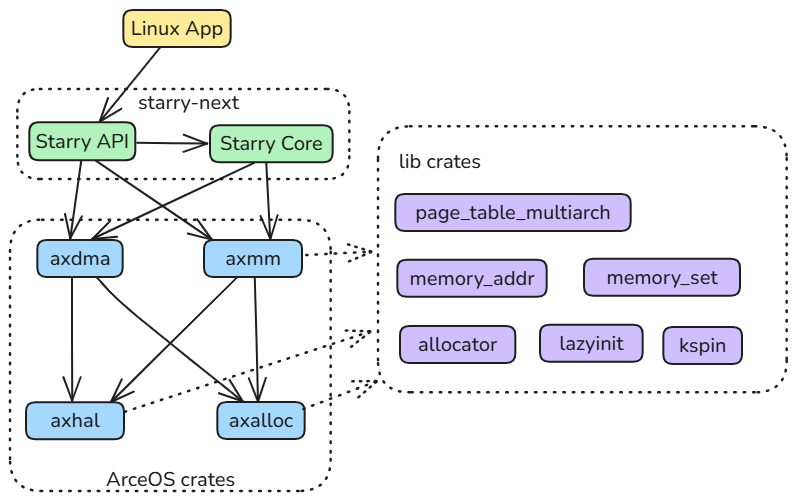
\includegraphics[width=0.7\linewidth, keepaspectratio]{subsystem2.png}
    \caption{内存管理子系统结构图}
    \label{fig:subsystem}
\end{figure}

如图\ref{fig:subsystem}所示,starry-next 中的 API 模块为应该提供系统调用支持,
并根据需要调用 Core 模块中的方法。而在这两个模块的功能又依赖于 ArceOS 中的模块,
例如 axmm 模块提供了内存管理的基本功能,axdma 模块提供了 DMA 相关的功能。
ArceOS 中的模块间也存在相互依赖关系,例如 axmm 和 axdma 依赖 axalloc 提供的全局内存分配器,
并且需要 axhal 提供不同架构的页表抽象相关功能和 axconfig 提供相关配置信息。
在 ArceOS 的下层,是 Rust 和第三方库的支持,例如 page\_table\_multiarch 提供了页表抽象的支持,
memory\_addr 和 memory\_set 提供内存地址和内存集合的抽象,lazyinit 和 kspin 提供了懒初始化和自旋锁的支持等。

内核启动后,先通过 axhal 和 axruntime 进行初始化,包括页表初始化、全局内存分配器的初始化和分配内核空间等。
然后启动 starry-next 的 main 函数,加载用户程序、分配用户空间和通过任务管理子系统进行任务调度。
在用户程序运行过程中,如果需要进行内存分配或释放等操作,则通过 mmap、munmap 等系统调用进入 starry-next 的 API 模块,
进而进入 ArceOS 的 axmm 等模块进行内存管理操作。
任务结束后,任务管理子系统会调用 axmm 等模块进行内存等资源的释放和回收。


\section{内存管理子系统直接相关的系统调用}

\subsection{mmap 系统调用}
mmap 用于将文件或设备内存映射到进程的地址空间。它在 Linux 和类 Unix 系统中广泛使用,主要用于高效地读写文件、实现内存共享以及分配匿名内存等。

mmap 系统调用的原型如下:


\begin{lstlisting}[language=C, caption=mmap 系统调用函数原型]
void *mmap(void addr[.length], size_t length, int prot, int flags, int fd, off_t offset);
\end{lstlisting}



可以看到,mmap 系统调用共有 6 个参数,其中 addr 和 length 用于指定内存映射的起始地址和长度,prot 用于指定内存映射的保护属性,flags 用于指定内存映射的标志,fd 用于指定要映射的文件描述符,offset 用于指定文件偏移量。当 addr 为 NULL 时,表示由内核自动选择内存映射的起始地址。在 Linux 中,内核会选择一个附近的页面边界,并尝试创建映射。如果该地址已经存在另一个映射,内核会选择一个新的地址。flags 参数决定了对映射区域的更新是否对映射同一区域的其他进程可见,以及更新是否会被写入底层文件,例如,MAP\_SHARED 标志表示对映射区域的更新对所有共享该映射的进程可见,而 MAP\_PRIVATE 标志则表示对映射区域的更新对其他进程不可见。

mmap 系统调用的返回值是一个指向内存映射区域的指针,该指针指向映射区域的起始地址。如果调用失败,返回值为 MAP\_FAILED(通常为 -1)。

内存映射主要分为两种类型:匿名映射是指不与任何文件关联的内存映射,通常用于分配动态内存,类似于 malloc,但提供了更多的灵活性和控制能力,例如多个进程可以共享同一个内存映射区域;文件映射是指将文件的内容映射到内存中,这样就可以像访问内存一样访问文件的内容,通常用于实现文件的高效读写。

如图\ref{fig:mmap}所示,在 starry-next 中,mmap 系统调用的实现主要包括以下几个步骤:首先解析参数并检查其有效性;然后进行地址对齐处理,根据是否指定映射起始地址选择将映射长度向上对齐到 4KB (页面大小)或将映射的起始和结束地址分别对齐到页面边界;接着确定映射的真正地址:如果 flag 中设置了 MAP\_FIXED 标志,则使用对齐后的 addr 地址作为映射的起始地址,并且如果 addr 和 length 指定的内存区域与任何现有的映射重叠,那么现有映射的重叠部分将被丢弃,否则,内核会在指定地址附近或者整个用户地址空间中寻找符合条件的空闲地址,并调用 AddrSpace 结构体的 map\_alloc 方法创建映射;最后返回起始地址;如果参数中 fd 不为 -1 且 MAP\_ANONYMOUS 标志未设置,即该映射是文件映射,则在返回前需要从文件中读取数据填充到内存中。

map\_alloc 是 ArceOS 提供的一个方法,用于创建内存映射。会先验证要映射的区域,然后创建一个新的内存区域,并将其映射到页表中。
在构建映射的过程中,会根据映射的类型(线性映射或分配映射),选择不同的后端进行处理。同时还需要为映射区域分配物理页,并在页表中记录。

\begin{figure}[H]
    \centering
    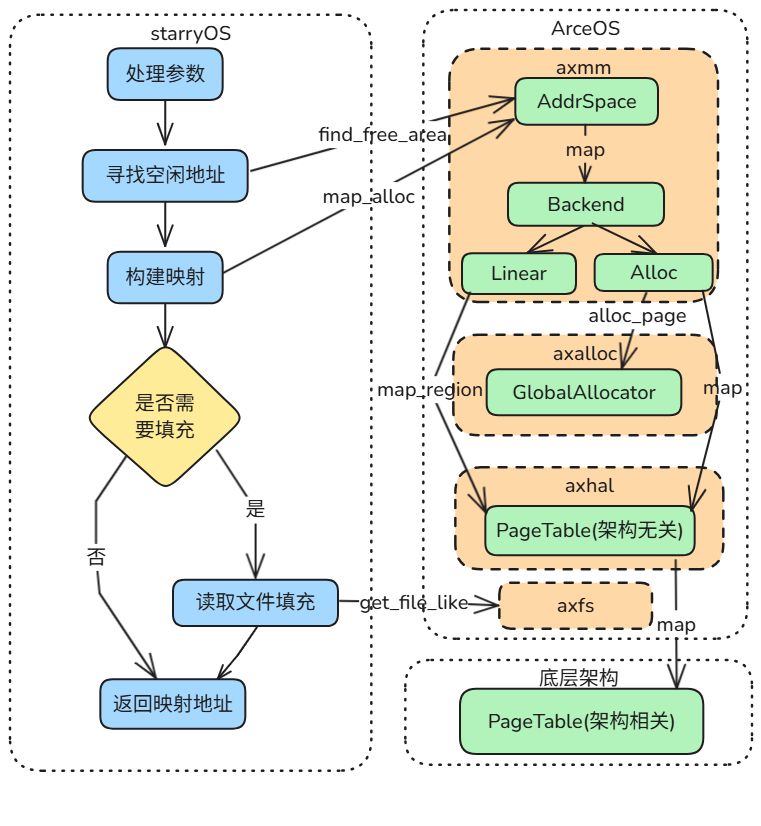
\includegraphics[width=0.7\linewidth, keepaspectratio]{syscall-mmap.png}
    \caption{mmap 系统调用流程}
    \label{fig:mmap}
\end{figure}


需要注意的是,由于 Lazy Map 机制的存在,不需要填充的内存区域不会立即被分配物理页,而是在第一次访问该内存区域并触发页面异常时才会分配物理页。该机制可能会导致内核在访问内存区域时出现 NotMapped 错误,因此需要在代码中调用 handle\_page\_fault 函数,为内存区域分配物理页,具体可以参考 AddrSpace 结构体的 clone\_or\_err 方法。

\begin{lstlisting}[language=c, caption=Lazy Map 机制下访问内存区域的处理]
let new_addr = match new_aspace.pt.query(vaddr) {
    Ok((paddr, _, _)) => paddr,
    // If the page is not mapped, try map it.
    Err(PagingError::NotMapped) => {
        if !backend.handle_page_fault(vaddr, area.flags(), &mut new\_aspace.pt) {
            return Err(AxError::NoMemory);
        }
        match new_aspace.pt.query(vaddr) {
            Ok((paddr, _, _)) => paddr,
            Err(_) => return Err(AxError::BadAddress),
        }
    }
    Err(_) => return Err(AxError::BadAddress),
};
\end{lstlisting}


除成功返回映射的起始地址外,starry-next 中 mmap 还有其他的返回情况:MAP\_FIXED 标志设置但地址为空,或者需要从文件读取数据填充映射区域但偏移量 offset 小于 0 或者超出文件大小,函数会返回 EINVAL 错误;若系统无法找到足够的连续空闲内存区域来完成映射操作,函数会返回 ENOMEM 错误;当需要从文件读取数据填充映射区域时,若文件描述符 fd 对应的文件对象无法转换为 arceos\_posix\_api::File 类型,函数会返回 EBADF 错误。

\subsection{munmap 系统调用}

munmap 用于解除进程地址空间中的内存映射。munmap 系统调用的原型如下:
\begin{lstlisting}[language=c, caption=munmap 系统调用函数原型]
int munmap(void addr[.length], size_t length);
\end{lstlisting}
munmap 系统调用共有 2 个参数,其中 addr 用于指定要解除映射的内存区域的起始地址,length 用于指定要解除映射的内存区域的长度。

munmap 系统调用的返回值是一个整数,通常为 0 表示成功,-1 表示失败。


如图\ref{fig:munmap},starry-next 中,munmap 系统调用的实现主要包括以下几个步骤:首先解析参数并检查其有效性;然后调用 AddrSpace 结构体的 unmap 方法,该方法会将指定的内存区域从页表中解除映射;刷新TLB;最后返回 0 表示成功。

\begin{figure}
    \centering
    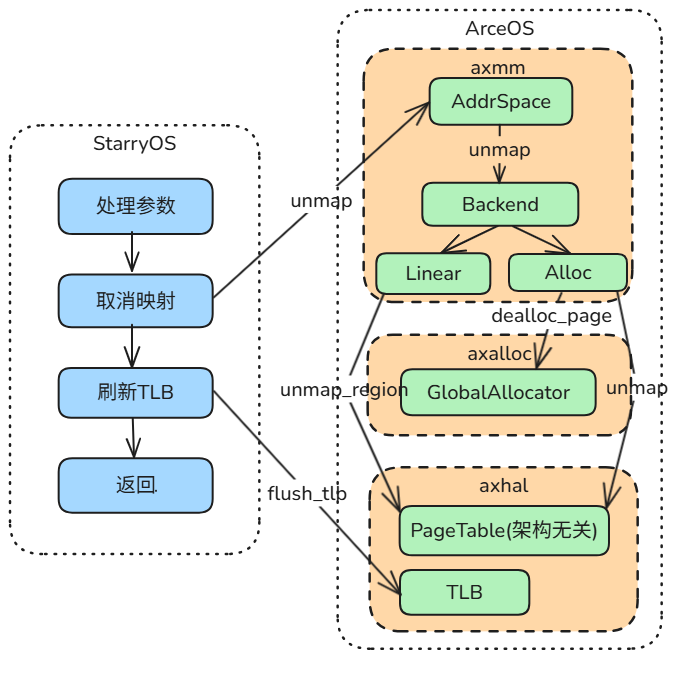
\includegraphics[width=0.7\linewidth, keepaspectratio]{syscall-unmap.png}
    \caption{munmap 系统调用流程}
    \label{fig:munmap}
\end{figure}


ArceOS 对 munmap 系统调用的支持方式与 mmap 系统调用类似,都是通过 AddrSpace 结构体向上提供接口,通过映射后端调用全局分配器和页表进行内存解除映射并释放物理页。 

另外,和 Linux 的标准实现相似,当需要取消映射的区域和当前存在的内存区域有重叠部分时,会将重叠部分的映射关系从页表中删除,并调整内存区域的起始地址和结束地址,如图\ref{fig:munmap2}所示,共存在三种情况:
\begin{enumerate}
    \item 完全覆盖:要解除映射的内存区域完全覆盖了当前存在的内存区域,此时需要将当前存在的内存区域从页表中删除,并将其从内存区域集合中移除。如图中第一项。
    \item 部分覆盖:要解除映射的内存区域位于当前存在的内存区域的中间部分,此时需要将当前存在的内存区域分为两部分,分别是要解除映射的内存区域的前半部分和后半部分,并加入到内存区域集合中,如图中第二项。
    \item 前后覆盖:要解除映射的内存区域包括当前存在的内存区域的左边界或右边界,需要调整当前存在的内存区域的起始地址或结束地址,如图中第三和第四项。
\end{enumerate}

\begin{figure}
    \centering
    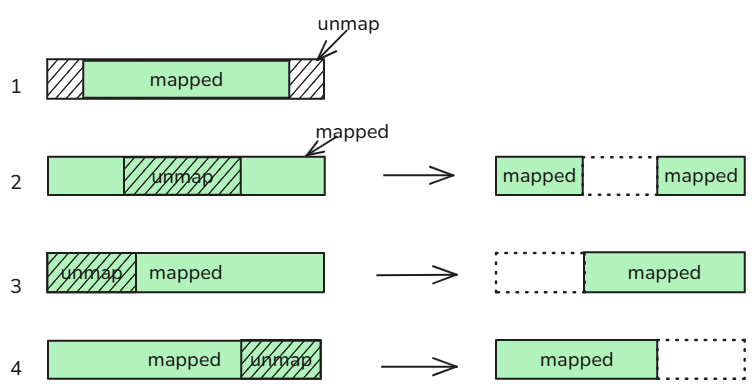
\includegraphics[width=0.7\linewidth, keepaspectratio]{syscall-munmap2.png}
    \caption{munmap 处理交叉区域}
    \label{fig:munmap2}
\end{figure}


\subsection{brk 系统调用}

brk 用于改变进程的堆顶位置。其原型如下:

\begin{lstlisting}[language=c, caption=brk 系统调用函数原型]
int brk(void addr);
\end{lstlisting}


可以看到,brk 系统调用只有一个参数,即 addr,用于指定数据段的结束位置。
其返回值是一个整数,通常为 0 表示成功,-1 表示失败。

starry-next 中,brk 系统调用通过设置任务信息结构体的 heap\_top 字段来改变堆顶地址。具体来说,brk 系统调用会将 heap\_top 字段设置为 addr,然后返回新的堆顶,但是如果 addr 小于当前 heap\_top,或者 addr 到堆底的距离大于进程的最大数据大小限制,那么 brk 系统调用会放弃设置新的堆顶并返回原来的堆顶地址。

需要注意的是,brk 系统调用只会改变进程的堆顶位置,并不会分配实际的物理内存。因此,在使用 brk 系统调用时,需要确保进程已经分配了足够的物理内存来支持新的堆顶位置。

\begin{figure}[H]
    \centering
    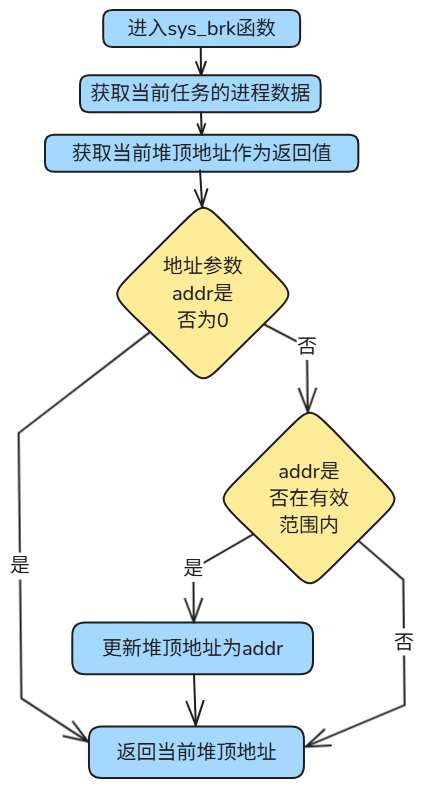
\includegraphics[width=0.4\linewidth, keepaspectratio]{syscall-brk-2.png}
    \caption{brk 系统调用流程}
    \label{fig:brk}
\end{figure}

\subsection{mprotect 系统调用}

mprotect 用于修改指定内存区域的保护属性。mprotect 系统调用的原型如下:
\begin{lstlisting}[language=c, caption=mprotect 系统调用函数原型]
int mprotect(void addr[.len], size_t len, int prot);
\end{lstlisting}

mprotect 系统调用接受三个参数:addr(要修改权限的内存区域的起始地址,必须是页面对齐的)、len(要修改权限的内存区域的长度)以及 prot(指定新的访问权限)。prot 参数可以是PROT\_NONE(无法访问)、PROT\_READ(可读取)、PROT\_WRITE(可写入)、PROT\_EXEC(可执行)、PROT\_GROWSDOWN(向下增长)、PROT\_GROWSUP(向上增长)的按位或组合。如果进程尝试以违反保护的方式访问内存,内核将生成一个 SIGSEGV 信号。

mprotect 系统调用的返回值是一个整数,通常为 0 表示成功,-1 表示失败。可能的错误包括:EFAULT——addr 指向的地址超出了进程的地址空间、EINVAL——len 为 0 或 prot 包含无效的标志、EACCES——进程没有足够的权限来修改内存区域的保护属性、ENOMEM——内存不足等。

如图\ref{fig:mprotect}所示,在进行地址长度页对齐等参数处理后,starry-next 使用了 AddrSpace 结构体的 protect 方法,进而通过 axhal 组件的页表接口来修改内存区域的保护属性。指定范围和当前存在的内存区域的关系和处理方式与 munmap 系统调用基本一致。但暂未实现 PROT\_GROWSDOWN 和 PROT\_GROWSUP 标志的处理。

\begin{figure}[H]
    \centering
    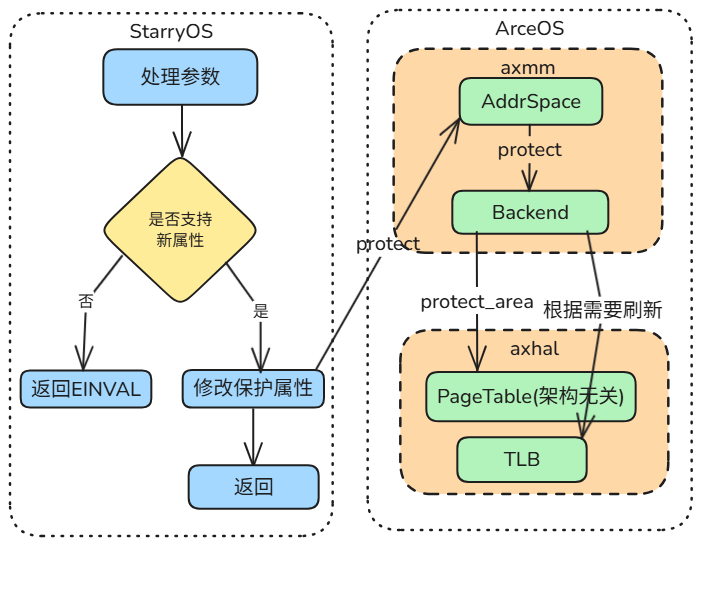
\includegraphics[width=1\linewidth, height = 8cm, keepaspectratio]{syscall-mprotect.png}
    \caption{mprotect 系统调用流程}
    \label{fig:mprotect}
\end{figure}

\section{内存管理子系统间接相关的系统调用}

\subsection{sysinfo 系统调用}

sysinfo 系统调用用于获取系统的信息,如内存使用情况、CPU 信息、文件系统信息等。sysinfo 系统调用的原型如下:
\begin{lstlisting}[language=c, caption=sysinfo 系统调用函数原型]
int sysinfo(struct sysinfo *info);
\end{lstlisting}
sysinfo 系统调用只有一个参数,即 info,用于存储系统信息的结构体指针。该结构体包含多个字段,例如 uptime(系统运行时间)、loads(1、5 和 15 分钟内的平均负载)、totalram 和 freeram(总内存和空闲内存)、sharedram 和 bufferram(共享内存和缓冲区内存)等。

% sysinfo 和内存管理的关系在于:sysinfo 系统调用可以获取系统的内存使用情况,包括总内存和空闲内存。因此在 ArceOS 的全局内存分配器的页分配器中,提供了接口以获取页分配器的总页数和空闲页数,这些信息可以用于计算总内存和空闲内存,并通过 sys\_sysconf 接口返回给 starry-next的 sysinfo 系统调用。

sysinfo 系统调用与包括内存管理在内的组件相关,例如通过 ArceOS 的 sys\_conf 接口获取 axconfig 组件中的核数等配置信息、axfs 组件的文件限制信息以及全局内存分配器的总页数和空闲页数;
通过 sys\_clock\_gettime 接口获取 axhal 组件的系统运行时间等。

\begin{figure}[H]
    \centering
    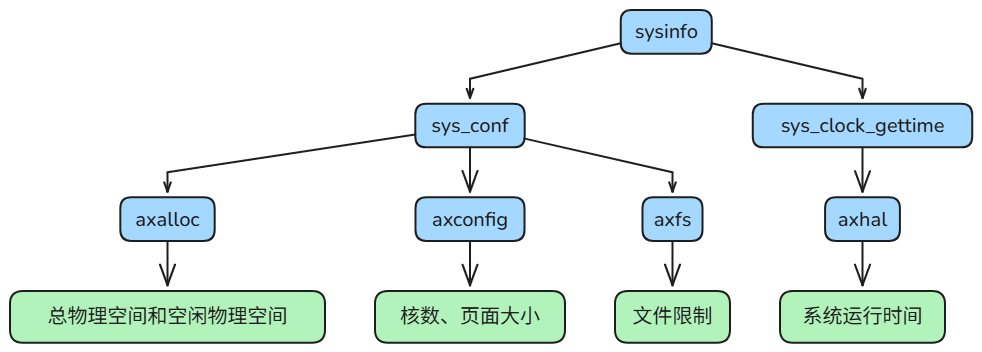
\includegraphics[width=1\linewidth, keepaspectratio]{syscall-sysinfo.png}
    \caption{sysinfo 系统调用流程}
    \label{fig:sysinfo-call}
\end{figure}

\subsection{arch\_prctl 系统调用}

arch\_prctl 系统调用用于设置或获取进程的特定架构相关的参数。其系统调用的原型如下:
\begin{lstlisting}[language=c, caption=arch\_prctl 系统调用函数原型]
int syscall(SYS_arch_prctl, int op, unsigned long addr);
int syscall(SYS_arch_prctl, int op, unsigned long *addr);
\end{lstlisting}

arch\_prctl 系统调用有两个参数,code 用于指定要设置或获取的参数,addr 用于指定参数的值,设置参数时会读取 addr 指向的内容,读取参数时将结果写入其指向的地址。常见的操作包括设置或获取进程的指针追踪(Pointer Tracing)状态、设置或获取 GS 段寄存器的值等。

arch\_prctl 系统调用的返回值是一个整数,通常为 0 表示成功,-1 表示失败。

当前 starry-next 中,arch\_prctl 系统调用支持四个参数的处理:GetFs、SetFs、GetGs 和 SetGs。其中 GetFs 和 SetFs 操作用于获取和设置进程的 FS 段寄存器的值,通过读取和设置 TrapFrame(陷阱帧)中的 TLS(Thread Local Storage,线程本地存储)寄存器实现;
GetGs 和 SetGs 操作用于读取和设置进程的内核 GS 段寄存器的值,通过读取和设置 x86 架构下 msr 寄存器实现。

\begin{figure}[H]
    \centering
    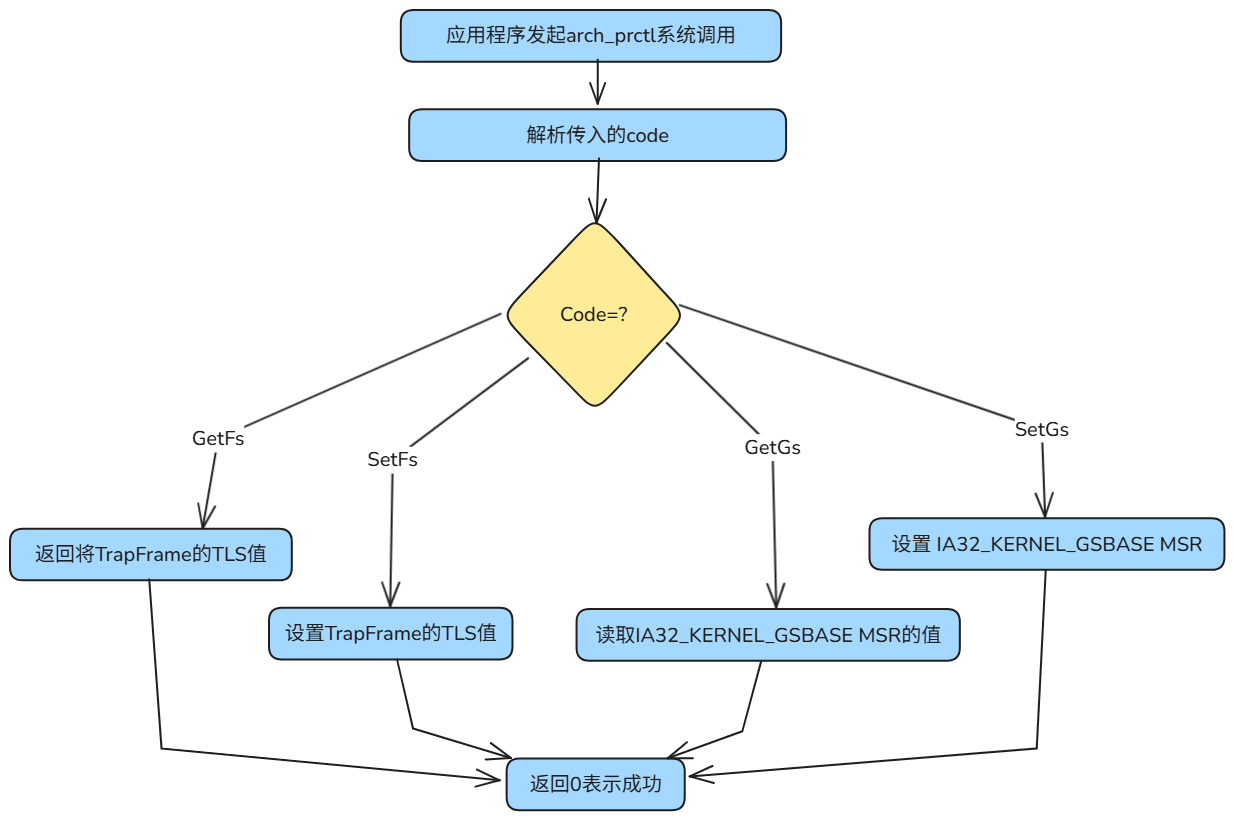
\includegraphics[width=1\linewidth, keepaspectratio]{syscall-arch-prctl-2.png}
    \caption{arch\_prctl 系统调用流程}
    \label{fig:arch-prctl}
\end{figure}

\subsection{prlimit64 系统调用}

prlimit64 系统调用用于设置或获取进程的资源限制,涉及操作系统的多个模块,例如栈大小和进程地址空间资源与内存管理模块有关,进程最大打开文件数与文件系统有关。prlimit64 系统调用的原型如下:
\begin{lstlisting}[language=c, caption=prlimit64 系统调用函数原型]
#include <sys/resource.h>
int prlimit64(pid_t pid, int resource, const struct rlimit64 *new_limit, struct rlimit64 *old_limit);
\end{lstlisting}

prlimit64 接受四个参数:pid——目标进程的进程ID,可以是当前进程或另一个进程)、
resource——要查询或设置的资源类型,例如 RLIMIT\_CORE(核心转储文件大小)、
RLIMIT\_CPU(CPU 时间)、RLIMIT\_DATA(数据段大小)等)、new\_limit——指向 rlimit64 结构体的指针,
用于指定新的资源限制,如果为 NULL 则表示仅获取当前限制,以及 old\_limit——指向 rlimit64 结构体的指针,
用于存储当前的资源限制,如果为 NULL 则不返回旧值。rlimit64 结构体包含 rlim\_cur(当前资源限制,又称软限制)和 rlim\_max(最大资源限制,
又称硬限制)两个字段,软限制是内核对相应资源强制执行的值,硬限制则作为软限制的上限。一个非特权进程只能将其软限制设置为从0到硬限制范围内的值,并且(不可逆地)降低其硬限制。

目前 starry-next 支持设置的资源限制包括 RLIMIT\_STACK(栈大小)和 RLIMIT\_NOFILE(最大打开文件数),二者分别通过修改进程信息结构体的 stack\_size 和 max\_files 字段来实现,其他类型的资源不会作处理。
同时限制了只有当前进程可以设置自己的资源限制,不能设置其他进程的资源限制,当传入的 pid 不为当前进程时,prlimit64 系统调用会返回 EINVAL 错误。

\begin{figure}[H]
    \centering
    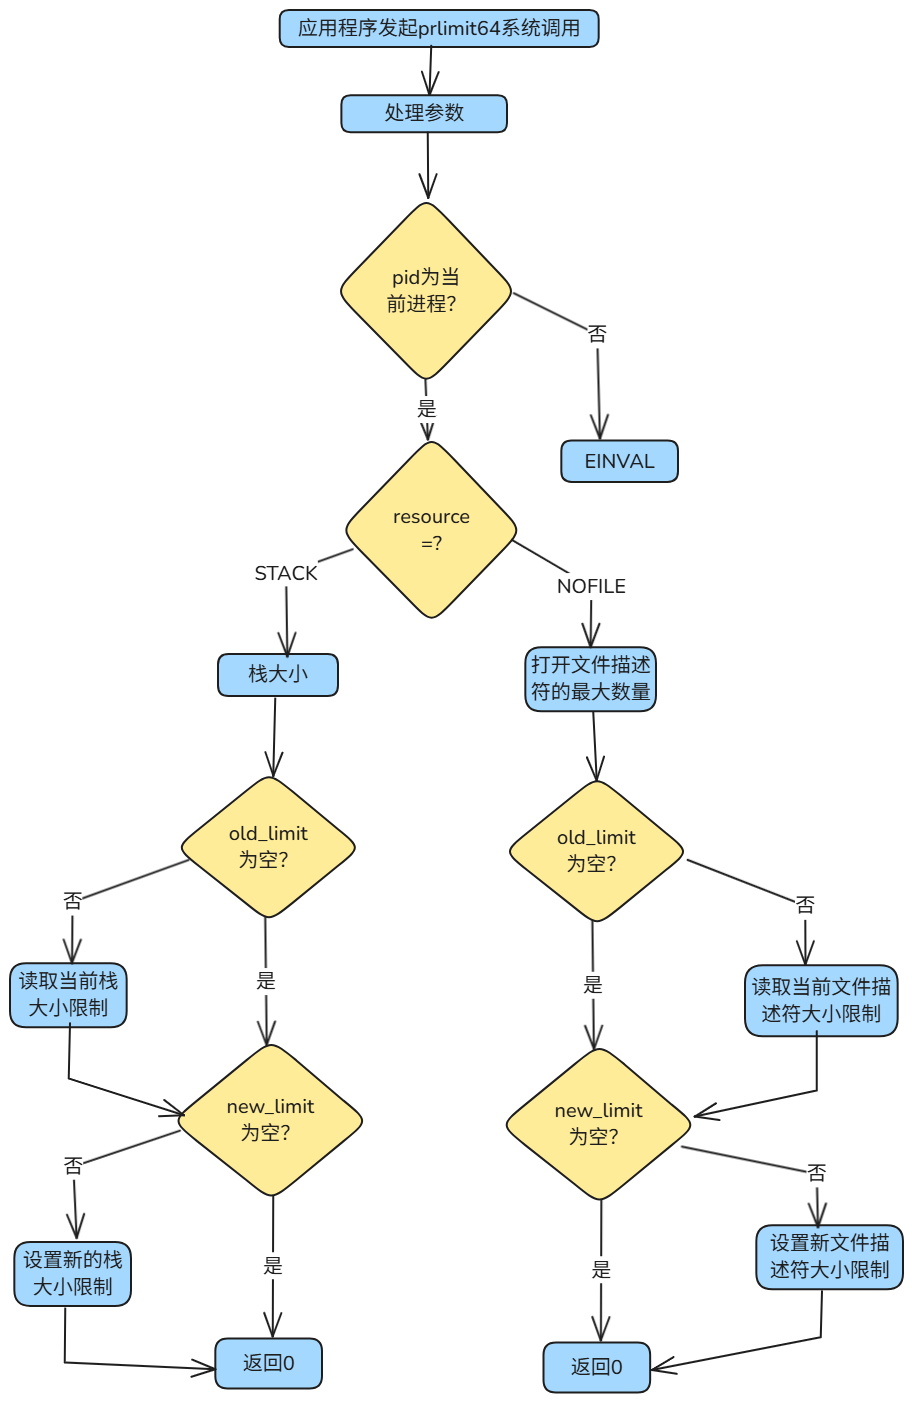
\includegraphics[width=0.7\linewidth, height=12.5cm]{syscall-prilimit64.png}
    \caption{prlimit64 系统调用流程}
    \label{fig:prlimit64}
\end{figure}

% !TeX root = ../cyh.tex

\chapter{实验环境与测试方法}

\section{实验环境}

% 本文采用 Linux 作为实验环境,使用 Ubuntu 20.04 作为主机操作系统,
为了验证 starry-next 内存管理模块及接口的设计与实现在 riscv64、x86\_64、loongarch64 和 aarch64 这四个架构下的正确性与性能,
我们使用了 qemu 模拟器来模拟这四个架构的运行环境,并且 qemu 模拟器的版本不应低于 8.2.0。qemu 是一个开源的虚拟机模拟器,支持多种硬件架构和操作系统,能够在主机上创建虚拟机并运行不同架构的操作系统。
同时,为了支持高版本的 qemu 模拟器,测例的本地运行都在 Ubuntu-24.04 下进行,并且需要在本地安装 rustling 工具链等 rust 相关工具,具体的操作可以参考项目的 README.md 文件。

另外,为了进行自动化测试,我们使用了 GitHub Actions 来实现自动化测试,定义了多个工作流配置文件,涵盖了不同架构和测试场景的自动化构建与验证。

测试分为功能测试和性能测试。

\section{功能测试}

\subsection{测试用例}

功能测试的测试用例分为两部分:开源测试用例和自定义测试用例。
其中开源测试用例主要来自 libc-test 库。libc-test 是一个针对 C 标准库(libc)功能及兼容性的检测工具。C 标准库作为 C 语言开发的基石,涵盖输入输出、内存管理、字符串操作等基础功能。
libc-test 借助一系列精心设计的测试用例,全面且细致地检验 C 标准库各功能模块,保障其在不同环境下的正确性和稳定性。在具体测试中,将编译完成的 libc-test 可执行文件作为输入,运行其中的静态与动态测试用例。
通过执行这些测试用例并检查输出结果,可判断待测内核是否能正确支持 C 标准库的各项功能,进而评估内核与 C 标准库的兼容性与稳定性。

尽管 libc-test 库提供了丰富的测试用例,可以涵盖大多数系统调用,例如 mmap、munmap、mprotect 等,但由于 libc-test 针对的是 C 标准库,而不是操作系统内核和系统调用的实现,
同时一部分系统调用无法使用 libc-test 进行测试,例如 sysinfo、prlimit64 等系统调用。
因此,我们还编写了一些自定义测试用例来验证 starry-next 内存管理模块的功能以及系统调用接口的正确性。这些用例将通过 C 标准库中 sys 子目录直接调用相关的系统调用,
并验证其返回值,例如:

\begin{lstlisting}[language=c, caption=prlimit64]
    #include <sys/syscall.h>
    syscall(SYS_prlimit64, getpid(), RLIMIT_STACK, NULL, &old_limit);
\end{lstlisting}

\begin{lstlisting}[language=c, caption=sysinfo]
    #include <sys/sysinfo.h>
    struct sysinfo info;
    sysinfo(&info);
\end{lstlisting}

在测例的编写和运行过程中,strace 指令可以帮助我们跟踪系统调用的执行情况,在 Ubuntu-24.04 下通过 strace 指令可以得到 x86\_64 架构下的系统调用信息,
使用 qemu 模拟器配合 strace 指令也可以得到其他架构下的系统调用信息。
这些不仅可以帮助验证测例的正确性,还可以作为对照组可以帮助我们分析 starry-next 内存管理模块的实现是否符合 Linux 的标准实现,
以及系统调用的实现的正确性,从而进行进一步的调试和优化。

\subsection{测试结果与分析}

接下来,我们将从系统调用的角度对测试结果进行展示与分析。

\subsubsection{mmap 和 munmap 系统调用}

要验证 mmap 系统调用的正确性,一方面可以通过本地使用 strace 指令在 libc-test 中找出使用了该系统调用的测试用例,例如 fdopen,这里我们展示 fdopen 测例在 x86\_64 架构下的测试结果:
\begin{lstlisting}[language=bash, caption=fdopen 测试结果]
    ========== START entry-static.exe fdopen ==========
    ...
    [  1.836930 1:11 starry::syscall:12] Syscall mmap
    [  1.838002 1:11 starry_api::imp::mm::mmap:100] mmap: addr: 0x0, length: 1000, prot: MmapProt(PROT_READ | PROT_WRITE), flags: MmapFlags(MAP_PRIVATE | MAP_ANONYMOUS), fd0
    [  1.845482 1:11 starry::syscall:145] Syscall mmap return 4096
    ...
    [  2.024200 1:11 starry::syscall:12] Syscall munmap
    [  2.027765 1:11 starry::syscall:145] Syscall munmap return 0
    ...
    Pass!
    ========== END entry-static.exe fdopen ==========
\end{lstlisting}

从结果中可以看到,fdopen 测试用例执行了 mmap 系统调用,创建一个长度为 1000 字节的匿名私有映射,这段内存区域可以被读取和写入。返回值为 4096,说明系统自动选择的起始地址是 0x1000,映射成功。
并且测例整体也是通过的,说明 mmap 系统调用匿名映射部分的实现是正确的。而 munmap 系统调用的返回值为 0,说明解除映射成功。

另一方面,我们还可以通过自定义测试用例来验证 mmap 系统调用的正确性,例如:
\begin{lstlisting}[language=c, caption=自定义 mmap 测试用例]
    fd = open("test_mmap.txt", O_RDWR | O_CREATE);
    array = mmap(NULL, kst.st_size, PROT_WRITE | PROT_READ, MAP_FILE | MAP_SHARED, fd, 0);
    printf("mmap content: %s\n", array);
\end{lstlisting}

在这个测试用例中,我们打开了一个文件,并使用 mmap 系统调用将该文件映射到内存中,然后读取文件内容并打印出来。
从运行结果来看,内核成功地将文件映射到内存中,并且可以正确读取文件内容,说明 mmap 系统调用的实现是正确的。

\begin{lstlisting}[language=bash, caption=自定义 mmap 测试用例结果]
========== START test_mmap ==========
file len: 27
mmap content:   Hello, mmap successfully!
========== END test_mmap ==========
\end{lstlisting}

\subsubsection{brk 系统调用}

brk 系统调用用于设置进程的堆空间的结束地址,因而要验证 brk 系统调用的正确性,可以通过反复设置和获取堆空间的结束地址来验证其实现是否正确。
例如 libc-test 中的 mbc 测试用例,在 x86\_64 架构下的测试结果如下: 
\begin{lstlisting}[language=c, caption=brk]
    [  1.817163 1:11 starry::syscall:12] Syscall brk
    [  1.819303 1:11 starry::syscall:145] Syscall brk return 1073741824
    [  1.821880 1:11 starry::syscall:12] Syscall brk
    [  1.823235 1:11 starry::syscall:145] Syscall brk return 1073750016
\end{lstlisting}

从结果中可以看到,brk 系统调用的返回值是 1073741824 和 1073750016,分别表示堆空间的结束地址是 1GB 和 1.5GB。
这说明 brk 系统调用的实现是正确的。

\subsubsection{sysinfo 和 prlimit64 系统调用}

sysinfo 和 prlimit64 系统调用的自定义测试用例主要是通过获取系统信息和进程限制来验证其实现是否正确。在 riscv64 架构下的测试结果如下:

\begin{figure}
    \centering
    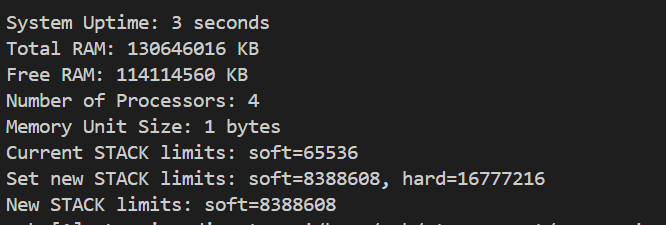
\includegraphics[width=0.5\linewidth]{sysinfo.png}
    \caption{sysinfo 和 prlimit64 测试结果}
    \label{fig:sysinfo-test}
\end{figure}

从图\ref{fig:sysinfo-test}中可以看到,sysinfo 系统调用返回了系统的内存使用情况,包括总内存和空闲内存等信息,并且 prlimit64 系统调用返回了进程用户栈的限制信息。
同时,当设置用户栈大小时,prlimit64 系统调用正确使用了新的软限制值,
这说明 sysinfo 和 prlimit64 系统调用用户栈选项的功能正常。而 prlimit64 的最大文件数量限制则可以通过 libc-test 的 rlimit\_open\_files 测试用例来验证,
该测例会在设置资源限制后重复创建新的文件描述符(打开文件)至失败,并取当前最大文件描述符和资源限制值进行比较,相等则说明实现正确。该测例也是通过的。

\begin{figure}
    \centering
    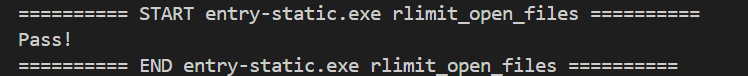
\includegraphics[width=0.5\linewidth]{prlimit64.png}
    \caption{rlimit\_open\_files 测例结果}
    \label{fig:prlimit64-test}
\end{figure}

\section{性能测试}

当前并未对 starry-next 内存管理模块的性能进行专项测试,
但在功能测试中,部分测例的运行时间也可以作为性能测试的参考。我们将 starry-next 内存管理模块的性能与 Linux 的标准实现进行对比,
以验证 starry-next 内存管理模块的性能是否符合 Linux 的标准实现。

以功能测试中的自定义 mmap 测试用例为例,
在 x86\_64 架构下的测试结果如下:
\begin{figure}[H]
    \centering  % 图片全局居中
    \begin{subfigure}[t]{0.45\textwidth}
        \centering
        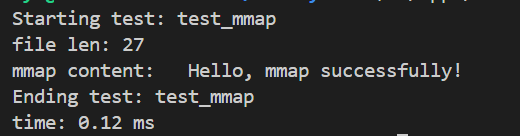
\includegraphics[width=\linewidth]{s2-local.png}
        \caption{Linux}
        \label{fig:sub.1}
    \end{subfigure}
    \hfill % 添加一些水平间距
    \begin{subfigure}[t]{0.45\textwidth}
        \centering
        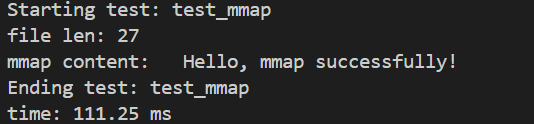
\includegraphics[width=\linewidth]{s2-starry.png}
        \caption{starry-next}
        \label{fig:sub.2}
    \end{subfigure}
    \caption{自定义 mmap 测试用例的运行时间对比}
    \label{Fig.main}
\end{figure}

不难看出,starry-next 花费的时间远高于本机的运行时间。为了减少其他模块的影响,
本文还设计了一个简单的 c 程序,该程序重复进行系统调用,
并将其运行时间与 Linux 的标准实现进行对比,
结果如下:

\begin{figure}[H]
    \centering  % 图片全局居中
    \begin{subfigure}[t]{0.45\textwidth}
        \centering
        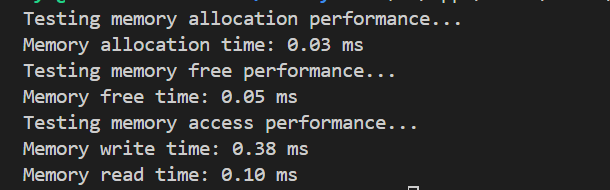
\includegraphics[width=\linewidth]{s1.png}
        \caption{Linux}
        \label{fig:sub.3}
    \end{subfigure}
    \hfill % 添加一些水平间距
    \begin{subfigure}[t]{0.45\textwidth}
        \centering
        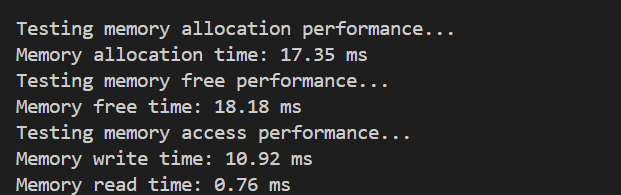
\includegraphics[width=\linewidth]{s1-starry.png}
        \caption{starry-next}
        \label{fig:sub.4}
    \end{subfigure}
    \caption{重复进行系统调用的运行时间对比}
    \label{Fig.main2}
\end{figure}

由图\ref{Fig.main2}可见starry-next 在映射、解除映射、读取和写入数据等方面花费的时间远高于本机的运行时间,
尽管 starry-next 的运行还要受到 qemu 模拟器的影响,自身也实现了 Lazy Map 等内存管理方面的优化机制,
但总体来说,其性能仍有很大的提升空间。
% !TeX root = ../cyh.tex

\chapter{结论与展望}

\section{结论}

到目前为止,我们已经基本完成了 starry-next 内存管理模块及其接口的设计与实现,并且对其进行了测试。我们的实现与 Linux 内核的内存管理模块接口基本一致,并且在功能测试中表现良好,
性能方面则需要进一步测试和优化。
具体的代码已开源至 \href{https://github.com/chenyihu21/starry-next}{GitHub}。

在开发过程中,由于操作系统的各模块间存在一定的依赖关系,
我们使用了多种协同开发 OS 的方法,包括使用 GitHub 的 issue 和 pull request 进行协作,
根据模块和系统调用分配任务,以通过某个测例为目的进行调试等。
我们不仅参与了宏内核接口的设计、实现与测试,还一定程度上参与了基座微内核 ArceOS 的修改。
另外,我们还将开发过程中的问题和解决方法记录在了实验报告中,以便后续的开发工作中可以参考。
希望这些工作能为后续组件化操作系统的开发提供一些参考和帮助。

\section{展望}

在未来的工作中,我们计划进一步完善 starry-next 内存管理模块及其接口,
包括完善当前仅实现部分功能的系统调用接口、优化内存管理模块的性能等方面。另外,当前 starry-next 内存管理模块还未支持各类页面置换算法,
我们计划在未来的工作中增加对不同页面置换算法的支持,以提高内存管理模块的性能和效率。
同时,增加对内存管理模块的安全性和稳定性的支持也会纳入未来的计划,
以确保内存管理模块在实际应用中能够稳定运行。

% 参考文献
\bibliography{myref/refs}  % 参考文献使用 BibTeX 编译
% \printbibliography       % 参考文献使用 BibLaTeX 编译

% 附录
\appendix
% % !TeX root = ../cyh.tex

\begin{survey}
\label{cha:survey}

\title{Title of the Survey}
\maketitle


\tableofcontents


本科生的外文资料调研阅读报告。


\section{Figures and Tables}

\subsection{Figures}

An example figure in appendix (Figure~\ref{fig:appendix-survey-figure}).

\begin{figure}
  \centering
  
\includegraphics[width=0.6\linewidth]{example-image-a.pdf}
  \caption{Example figure in appendix}
  \label{fig:appendix-survey-figure}
\end{figure}


\subsection{Tables}

An example table in appendix (Table~\ref{tab:appendix-survey-table}).

\begin{table}
  \centering
  \caption{Example table in appendix}
  \begin{tabular}{ll}
    \toprule
    File name       & Description                                         \\
    \midrule
    thuthesis.dtx   & The source file including documentation and comments \\
    thuthesis.cls   & The template file                                   \\
    thuthesis-*.bst & BibTeX styles                                       \\
    thuthesis-*.bbx & BibLaTeX styles for bibliographies                  \\
    thuthesis-*.cbx & BibLaTeX styles for citations                       \\
    \bottomrule
  \end{tabular}
  \label{tab:appendix-survey-table}
\end{table}


\section{Equations}

An example equation in appendix (Equation~\eqref{eq:appendix-survey-equation}).
\begin{equation}
  \frac{1}{2 \uppi \symup{i}} \int_\gamma f = \sum_{k=1}^m n(\gamma; a_k) \mathscr{R}(f; a_k)
  \label{eq:appendix-survey-equation}
\end{equation}


\section{Citations}

Example\cite{dupont1974bone} citations\cite{merkt1995rotational} in appendix
\cite{dupont1974bone,merkt1995rotational}.


% 默认使用正文的参考文献样式;
% 如果使用 BibTeX,可以切换为其他兼容 natbib 的 BibTeX 样式。
\bibliographystyle{unsrtnat}
% \bibliographystyle{IEEEtranN}

% 默认使用正文的参考文献 .bib 数据库;
% 如果使用 BibTeX,可以改为指定数据库,如 \bibliography{ref/refs}。
\printbibliography

\end{survey}
       % 本科生:外文资料的调研阅读报告
% !TeX root = ../cyh.tex

\newcommand{\OSname}{Ariel~OS}
\newcommand{\espcthree}{ESP32\nobreakdash-C3}
\newcommand{\espsthree}{ESP32\nobreakdash-S3}
\newcommand\noteEB[1]{\textcolor{red}{EB: #1}}
\newcommand\noteEF[1]{\textcolor{blue}{EF: #1}}
\newcommand\noteKS[1]{\textcolor{brown}{KS: #1}}
\newcommand\noteKZ[1]{\textcolor{navy}{KZ: #1}}
\newcommand\noteCA[1]{\textcolor{gray}{CA: #1}}
\begin{translation}
\label{cha:translation}

\title{Ariel OS:适用于网络传感器和多核微控制器的嵌入式Rust操作系统}
\maketitle

\begin{abstract}
% Large swaths of low-level system software building blocks originally implemented in C/C++ are currently being swapped for equivalent rewrites in Rust, a relatively more secure and dependable programming language. 
% %Such re-implementations are primarily motivated by the comparatively increased dependability provided by software modules written in Rust.
% %The C to Rust migration concerns not only software running on microprocessors, but also software embedded on microcontrollers. Indeed, 
% %In this context, a trend emerged whereby new operating systems targeting microcontrollers are based on embedded Rust. However, 
% %Although networked sensors increasingly use new microcontrollers based on multicore 32-bit hardware architectures,
% So far, however, no embedded OS in Rust 
% %available embedded Rust operating systems 
% supports multicore preemptive scheduling on microcontrollers.
% % such as found on networked sensors' hardware.
% %However, in order to fully exploit the potential for distributed  computing in  the  Internet  of  Things (IoT), efficient multicore support is a must.
% In this paper, we thus fill this gap with a new operating system:  \OSname{}. % supporting multicore scheduling (symmetric multiprocessing) and improves application code portability on diverse popular 32-bit microcontroller architectures.
% We describe its design, we provide the source code of its implementation, and we perform micro-benchmarks on the main 32-bit microcontroller architectures: ARM Cortex-M, RISC-V and Espressif Xtensa. 
% We show how our scheduler takes advantage of several cores, while incurring only small overhead on single-core hardware. 
% %\OSname{} also integrates a curated set of libraries (various Rust crates for crypto, network stacks, and other system utilities). 
% %These can be cherry-picked at compile time, made accessible via APIs we crafted such that they remain consistent across different hardware.
% As such, \OSname{} provides a convenient embedded software platform for small networked devices, for both research and industry practitioners.
% %with a view to conveniently develop over a more dependable software basis with embedded Rust on networked sensors using microcontrollers.
% %On the one hand, researchers can more easily carry out experiments exploiting the features of a larger matrix of recent (and less recent) microcontroller hardware.
% %On the other hand, by using \OSname{}, a company could accelerate a transition from C towards embedded Rust software, while maintaining a high level of agility in terms of reusing software (e.g. their business logic) on a wide variety of microcontroller architectures and boards available commercially off-the shelf.

大量原本用C/C++实现的低级系统软件组件,目前正在被用Rust语言重新编写。Rust是一种相对更安全、更可靠的编程语言。然而,到目前为止,还没有用Rust编写的嵌入式操作系统支持微控制器上的多核抢占式调度。因此,本文填补了这一空白,提出了一个新的操作系统:Ariel OS。我们描述了它的设计,提供了其实现的源代码,并在主流的32位微控制器架构上进行了微基准测试,包括ARM Cortex-M、RISC-V和Espressif Xtensa。我们展示了我们的调度器如何在利用多核优势的同时,仅在单核硬件上产生极小的额外开销。正因如此,Ariel OS 为研究和行业从业者针对小型联网设备提供了一个便捷的嵌入式软件平台。
\thusetup{
    keywords = {嵌入式软件、Rust、微控制器、多核、操作系统、实时操作系统(RTOS)、物联网(IoT)},
  }
\end{abstract}

% \tableofcontents

% \begin{IEEEkeywords}
% % Embedded Software, Rust, Microcontroller, Multicore, Operating System, RTOS, Internet of Things, IoT 
% 嵌入式软件、Rust、微控制器、多核、操作系统、实时操作系统(RTOS)、物联网(IoT)
% \end{IEEEkeywords}




\section{引言}

我们对网络物理系统(cyberphysical systems)和分布式计算系统的依赖程度日益加深。这些系统所涵盖的硬件不仅包括微处理器领域的机器,还涵盖了更多资源受限的设备,例如基于微控制器单元(MCU)的传感器。根据 RFC7228~\cite{rfc7228} 的描述,这些设备实现了超低功耗和超低价格,但与微处理器相比,它们的内存容量要小得多(仅在\emph{千字节}范围内),处理能力也弱得多(CPU 时钟速度在\emph{兆赫兹}范围内)。

\textbf{众多的多核微控制器——} 为了在设备保持可用以进行传感、驱动或通过网络进行数据推送/拉取的同时,执行计算密集型任务(例如实时音频处理或边缘机器学习,%(例如 TinyML 或后量子密码学)
),必须高效利用多核。这些任务需要在设备板上执行。因此,许多厂商的旗舰产品如今都基于多核 32 位架构。例如,%Nordic nRF53 微控制器基于双核 ARM Cortex-M33,被用于流行的 Thingy53 开发板;
Espressif ESP32\nobreakdash-S3 微控制器基于双核 Xtensa LX7;RP2350 微控制器基于双核 RISC-V Hazard3 和双核 ARM Cortex\nobreakdash-M33,被用于流行的 Raspberry Pi Pico 2 开发板。早期型号 RP2040 基于双核 ARM Cortex\nobreakdash-M0+,已经售出数百万个单位。
其他厂商(如 Nordic、NXP、ST 等)也推出了 32 位多核微控制器。



\textbf{微控制器的嵌入式操作系统——} 随着在微控制器(MCU)和传感器上运行的软件日益复杂,操作系统(OS)的使用变得愈发普遍。目前,最知名的操作系统大多采用C语言编写,例如 RIOT、Zephyr 和 FreeRTOS~\cite{hahm2015operating}。近年来,随着 Rust 语言的兴起,一种新型的操作系统和嵌入式软件平台应运而生,它们以 Rust 语言为核心进行开发。

% This effort was pioneered by Tock~OScite{levy2015ownership} and many \emph{bare-metal} embedded Rust programming efforts, which resulted in vastly improved embedded Rustcite{embedded-rust-book}. 
这一领域的先驱工作由 Tock~OS\cite{levy2015ownership} 和众多 \emph{裸机} 嵌入式 Rust 编程项目引领,这些工作极大地提升了嵌入式 Rust 的性能和可靠性~\cite{embedded-rust-book}。
%Beyond Tock~OS, e
% Examples of embedded Rust platforms for MCUs
% include Hubris~\cite{hubris}, Drone~OS~\cite{drone-os}, RTIC~\cite{rtic}, as well as  asynchronous Rust with Embassy~\cite{embassy}. %Another example is RIOT-rs~\cite{riot-rs}, a rewrite of RIOT in Rust). \noteEF{Should we still mention RIOT-rs?}
% However, to date, none of these support multicore scheduling on the main 32-bit microcontrollers.
适用于微控制器的嵌入式 Rust 平台示例包括 Hubris~\cite{hubris}、Drone~OS~\cite{drone-os}、RTIC~\cite{rtic},以及支持异步编程的 Embassy~\cite{embassy}。%另一个例子是 RIOT-rs~\cite{riot-rs},即用 Rust 重写的 RIOT。 \noteEF{我们是否仍需提及 RIOT-rs?}
然而,迄今为止,这些平台中尚无一个支持在主流 32 位微控制器上进行多核调度。
%This is a small part of a larger movement knownw as \textit{RIIR} (Rewrite It In Rust), which is driven by calls~\cite{potus} for a fundamental shift towards using a more secure and dependable basis than C/C++ building blocks. It thus looks like Rust might fuel the future more than C/C++.
\iffalse
The so-called ownership model in Rust can conflict with common resource-sharing practices used in embedded systems to fit smaller memory budgets, thus requiring new workarounds to maintain memory safety guarantees~\cite{levy2015ownership}. Despite such challenges Rust is attractive for developing less vulnerable embedded software, because of its memory safety features (as well as more convenient abstraction and more modern tooling, compared to C).
\fi





% The Raspberry Pi Pico} is the first microcontroller by Raspberry Pi, with the dual Cortex M0+ RP2040 chip.
% https://www.raspberrypi.com/news/raspberry-pi-pico-2-our-new-5-microcontroller-board-on-sale-now/
% It was released in 2021 and since then has been sold nearly 4 million times [CITE].
% It is commonly used in the Internet of Things, e.g., in LoRaWAN networks \cite{LoRaWAN-RP2040}, for on-device machine learning \cite{TinyML-RP2040, tinyml-healthcare, tinyRL-RP2040}, or in healthcare \cite{IoMT-RP2040, tinyml-healthcare}.

%\textbf{The ESP32-S3} with dual Xtensa LX7 cores has been specifically designed for the Artificial Internet of Things (AIoT) that has gained great relevance in recent years. It is used, e.g., for Human Activity Recognition (HAR) \cite{HAR-audio-data, HAR-wifi-csi} or environmental monitoring \cite{environmental-monitoring}.


\iffalse

\textbf{Lacking embedded Rust OS support for multicore -- } The bulk of recent efforts on embedded Rust has been dedicated to asynchronous (async) Rust, i.e. cooperative multi-tasking without threads/scheduler, for instance as provided by Embassy~\cite{embassy}. Surprisingly, however, none of the embedded Rust OS or frameworks support multicore scheduling to this day---while several older OS written in C/C++ do.
In fact, this gap becomes problematic because a large part of the newer MCU architectures that appear on the market nowadays are multicore---and this trend is here to stay. 

Exploiting multicore efficiently is required to allow the execution of computation-intensive tasks, %(e.g. TinyML or post-quantum cryptography)  which must be executed on-board 
while the device remains available for sensing, actuation, or push/pull of data over the network. For instance, dual-core microcontrollers such as RP2040 or dual-core Xtensa LX7 are commonly used in Internet of Things, e.g., in LoRaWAN networks~\cite{LoRaWAN-RP2040}. Similar hardware is used for on-device machine learning~\cite{TinyML-RP2040, tinyml-healthcare, tinyRL-RP2040}, in healthcare~\cite{IoMT-RP2040, tinyml-healthcare}, for Human Activity Recognition (HAR)~\cite{HAR-audio-data, HAR-wifi-csi} or for environmental monitoring~\cite{environmental-monitoring}. Multicore scheduling is therefore a \emph{must-have} to exploit to its full potential the capacities of distributed computing in the IoT.

\fi 

% Aiming to bridge this gap:
%our paper presents \OSname{}, the first embedded Rust operating system combining a multicore scheduler and asynchronous (async) Rust. %Note that in this paper, we focus on SMP, not on AMP.
%In this context, the work we present next in 
%\textbf{our paper contributes the following}:
% \begin{itemize}
%     \item We design 1, a novel embedded Rust operating system combining
%     \begin{enumerate*}[label=(\roman*)]
%         \item a scheduler exploiting single- and multicore  microcontrollers, and 
%         \item asynchronous Rust;
%     \end{enumerate*}% based on Symmetric Multiprocessing (SMP);
% %    \item We implement \OSname{} and we detail how the implementation takes advantage of Rust characteristics;
%     \item We implement 1 and provide benchmarks on diverse 32-bit microcontroller architectures: ARM \mbox{Cortex\nobreakdash-M}, Espressif Xtensa, and RISC-V;
%  %   \item We provide micro-benchmarks using \OSname{} on different microcontroller architectures;%, which demonstrate substantial benefits and negligible overhead of multicore scheduling, compared to single-core use;
%     \item We overview the OS, which, beyond the scheduler, integrates diverse libraries and cross-hardware APIs;
%     \item We publish the full 1 code as open source. % including the micro-benchmark code.
    
% \end{itemize}

为了填补这一空白:
%我们的论文介绍了 \OSname{},这是首个结合了多核调度器和异步(async)Rust 的嵌入式 Rust 操作系统。%请注意,在本文中,我们关注的是对称多处理(SMP),而不是非对称多处理(AMP)。
%在此背景下,我们在本文中介绍的工作
%\textbf{我们的论文做出了以下贡献}:
\begin{itemize}
    \item 我们设计了 \OSname{},这是一个创新的嵌入式 Rust 操作系统,它结合了以下特性:
    \begin{enumerate}[label=(\roman*)]
        \item 针对单核与多核微控制器优化的调度器;
        \item 异步 Rust;
    \end{enumerate}% 基于对称多处理(SMP);
%    \item 我们实现了 \OSname{},并详细说明了实现如何利用 Rust 的特性;
    \item 我们实现了 \OSname{},并在多种主流 32 位微控制器架构上进行了性能测试,包括 ARM \mbox{Cortex\nobreakdash-M}、Espressif Xtensa 和 RISC-V;
%   \item 我们在不同的微控制器架构上使用 \OSname{} 提供了微基准测试;%,这些测试展示了与单核使用相比,多核调度的显著优势和微不足道的开销;
    \item 们对操作系统进行了全面概述,它不仅包含调度器,还集成了多种库和跨硬件的 API;
    \item 我们将 \OSname{} 的完整代码开源发布。% 包括微基准测试代码。
    
\end{itemize}
% %\subsection{Related Work}
\label{sec:related-work}
% - Related work in context of scheduling 
% - What support is in RTOSes
% (condensed from thesis)


%Prior work on schedulers leveraging the multicore capacity on such hardware includes three main areas, i.e. literature on (i)  multicore scheduling algorithms/schemes, (ii) multicore scheduling support on microcontrollers and (iii) embedded Rust software platforms.

\textbf{Multicore Scheduling Schemes ---} The traditional approach to multicore scheduling is to adapt uniprocessor real-time scheduling algorithms such as Earliest Deadline First (EDF) or Rate Monotonic (RM).
The main categories of approaches are global, partitioned, or hybrid scheduling. The performance of global vs. partitioned EDF and RM scheduling was studied in~\cite{P-PF-partition-or-not, hardrealtime-multiprocessor-survey, GRMS, EDF-RM-multiprocessor-survey}. These indicate global scheduling is a better fit for soft real-time, while partitioned scheduling is a better fit for hard real-time and/or cases with a large number of cores.
\iffalse
Their findings are that global scheduling is generally more favorable for soft real-time systems because it can balance out individual deadline misses. 
Partitioned scheduling, on the other hand, is more suited for hard real-time systems because deadline misses on one core won’t affect any of the other cores. 
Furthermore, they showed that partitioned schemes scale better for a large processor count.
\fi
Other scheduling schemes include clustered or semi-partitioned scheduling~\cite{brandenburg, hardrealtime-multiprocessor-survey, energy-efficient-sched-for-HRT}, as well as schemes that specifically consider inter-task dependencies~\cite{allocate-dags-to-multiprocessors, shared-resources-coolocation, scheduling-task-on-heterogenous-multicore, mapping-in-multicore, resource-oriented-partitioned-scheduling} or power usage~\cite{scheduling-for-low-power-platforms}.

\textbf{Multicore Scheduling on Microcontrollers ---} Widely used operating systems providing thread schedulers in the microcontroller segment include Zephyr~\cite{zephyr}, FreeRTOS~\cite{freertos}, RIOT~\cite{baccelli2018riot}, ThreadX~\cite{threadx}, or Contiki~\cite{dunkels2004contiki}, and others surveyed for instance in~\cite{hahm2015operating}. These OS are primarily written in C---although some started to include Rust modules marginally~\cite{riot-wrappers}.
Some OS offer configurations supporting multicore scheduling, 
%Specifically, we surveyed the implementation in
for instance FreeRTOS, ThreadX, Zephyr, NuttX~\cite{nuttx}, and RT-Thread~\cite{rt-thread}. None of these are written in Rust.


\textbf{Embedded Rust Software Platforms ---} A number of embedded Rust operating systems has emerged over the last years. 
The most prominent ones are Tock OS~\cite{levy2017tock} and Hubris~\cite{hubris}. RIOT-rs~\cite{riot-rs} is a rewrite of RIOT in Rust. %\noteCA{Should this reference point to a version when it was still a rewrite in its early stage? The repo there is an October 2024 version, which is already more Ariel than a RIOT rewrite.}\noteKS { IMO the point just before multicore was merged is fine (or close to that, whatever Elena chose). those early days were super experimental ...}. 
Other operating systems include for instance Drone OS~\cite{drone-os} %Bern RTOS 
or R3-RTOS~\cite{r3-rtos} and others surveyed in~\cite{vandervelden2024rust-os}.
Last but not least, two prominent concurrency frameworks, RTIC~\cite{rtic} and Embassy~\cite{embassy}, are well known embedded software platforms for applications with concurrent tasks. 
Both lack a software kernel however, and provide limited portability.
%\noteCA{RTIC before 2.0 was not async based, and may warrant some consideration; in a sense, it did offer a form of scheduling, but with a very limited scope.}
% Concerning portabilit: I'm referring here to the fact that its not possible to simply compile the same application for another target, since individual configurations, initialization and dependencies must be changed. Can this be expressed better?
% We observe that none of the embedded Rust operating systems support multicore scheduling.
%Embassy supports some level of multiple core usage: on the RP2040 and ESP32 families, 
In particular, Embassy is a popular framework using async Rust (instead of threads and scheduling) and enables manual spawning of a task executor on a second core on RP2040 and ESP32 families (but no multicore scheduler). %While this somewhat resembles a partitioned scheduling scheme, basic scheduling features such as priority-based scheduling or separate task stacks are not supported \noteKS { But executors do have separate stacks? }. 
%\noteEF{ But not separate stacks per task }.
% Mention and give references for Tock OS~\cite{levy2017tock}, Drone~OS, Hubris, Drogue, and others surveyed for instance in~\cite{vandervelden2024rust-os}.
% Mention and distinguish also HAL/frameworks such as RTIC, Embassy~\cite{embassy}.
% We observe that none of the embedded Rust software plaftorms support multicore scheduling.



\iffalse
\section{Additional Background on Schedulers}
\label{sec:background}

%Scheduler-savvy readers can skip this section. 
Scheduling describes the process of assigning a program's units of execution---i.e. \textit{threads}---to the available processors (\emph{cores}).
When a thread executes on a processor, it runs until it either cooperatively stops its own execution (\textit{yielding}) or is interrupted mid-execution by the scheduler (\textit{preemption}).
In both of these cases, the scheduler is invoked through a processor exception that interrupts normal thread execution, switches the processor into interrupt mode, and executes the scheduler interrupt handler.

This handler performs a \textit{context switch}.
A context switch describes the process of saving the state of the previously running thread, i.e., saving its program counter and register state, and loading the state of the next thread from its \textit{Thread Control Block} (TCB).

The loaded state of the next thread is the exact state that thread was in when it was last interrupted.
In \textit{real-time scheduling}, each thread has a priority that affects when it is scheduled.
The scheduler must prioritize the execution of higher priority threads over the execution of lower priority ones.
Same priority threads are either scheduled in a \textit{time-sliced} fashion, or---in case of a \textit{tickless} scheduler---cooperatively.
Ready, waiting threads are listed in a sorted data structure called the \emph{runqueue}, whereby the head of the runqueue is the thread that should be executed next.

To prevent conflicting accesses to shared resources and data races, \emph{critical sections} can be used to implement mutual exclusion for a resource between threads.
While one thread is executing a critical section, no other critical section may be entered by another thread.
Furthermore, synchronization and Inter-Process Communication (IPC) between thread is commonly implemented through primitives such as thread flags---per-thread bitmasks---channels or locks. For further reading, we refer to~\cite{hardrealtime-multiprocessor-survey,Bos2023}.
%\noteCA{My layman's impression is that both critical sections and atomics are viable for implementing mutual exclusion. Was that a choice made here? If so, might say ``data races, \em{we choose} critical sections to implement''} \noteKS{ Uh, definition time ... Atomics on their own can only do mutual exclusion through spinning / busy looping (or going non-blocking try\_lock). and be used to implement critical sections}

% \noteEB{how about also introducing terms: synchronization, critical section? }
% \noteEF{Done critical section. Not sure if we need to explain sychronization; kinda difficult to do it without using the term itself.}
When transitioning from single- to multicore scheduling, the main challenges are
\begin{enumerate*}[label=(\roman*)]
\item the efficient distribution of the threads to the available cores, 
\item avoiding race conditions in the scheduler, 
\item maintaining a low overhead for cross-core runqueue maintenance, and 
\item avoiding idle cores and priority inversions.
\end{enumerate*}
% (i) minimizing the overhead of cross-core runqueue maintenance and (ii) determining efficiently which core a given thread should be assigned to. 
% \noteEB{can someone review/improve the above?}
%\noteEF{I find it hard to decide what to include here and what not. 4 aspects are maybe too much? Feel free to reorder or cut down parts of it.}
% context/TCB, Runqueue, Tickless, Preemptive, fixed priority, context switch, Async Tasks vs scheduled Threads



%  Background in global scheduling impl in other OSes (ThreadX, FreeRTOS etc) -> move details from Related Work Section

\fi

\section{微控制器上的多核调度的相关研究} \label{sec:multicore-sched}


% Surveying existing software and prior literature, we found that notable examples of multicore scheduling on microcontrollers include ThreadX~\cite{threadx} and FreeRTOS~\cite{freertos}, Zephyr~\cite{zephyr} and NuttX~\cite{nuttx}.
% %we listed in Section \ref{sec:related-work}, 
% Typically, threads that are ready and waiting for execution are listed  in a sorted data structure called the \emph{runqueue}. %whereby the head of the runqueue is the thread that should be executed next.
% We observe two main approaches for runqueues on multicore architectures. The first approach, \textit{global scheduling}, uses a single global runqueue from which the threads are distributed onto the available cores.
% In contrast, the \textit{partitioned scheduling} approach employs separate runqueues for each processor, to which threads are statically allocated.
% Furthermore, we observed that OSs for microcontrollers that support multicore scheduling primarily use global scheduling.
% We also observed that for synchronization within the scheduler, global critical sections are typically used.

在对现有软件和相关文献进行调研后,我们发现微控制器上的多核调度的显著示例包括 ThreadX~\cite{threadx} 和 FreeRTOS~\cite{freertos},以及 Zephyr~\cite{zephyr} 和 NuttX~\cite{nuttx}。
%我们在第 \ref{sec:related-work} 节中列出了这些内容,
通常,处于就绪状态且等待执行的线程会被列入一个称为 \emph{运行队列}(runqueue)的有序数据结构中。%运行队列的头部是下一个将被执行的线程。
我们观察到在多核架构上,运行队列主要有两种方法。第一种方法是 \textit{全局调度},它使用一个单一的全局运行队列,线程从该队列中被分配到可用的核上。
相比之下,\textit{分区调度} 方法为每个处理器使用单独的运行队列,线程被静态分配到这些队列中。
此外,我们还观察到,支持多核调度的微控制器操作系统主要使用全局调度。
我们还发现,在调度器内部进行同步时,通常会使用全局临界区。

% We finally observed that operating systems in this space employ different approaches for assigning threads to cores. 
% On the one hand ThreadX uses a \textit{core reallocation approach}, whereby a reallocation routine maps the \textit{n} highest priority threads to the \textit{N} cores. 
% % The allocation for each core is stored in an array that the scheduler interrupt handler reads upon invocation. 
% The allocation for each core is read by the scheduler interrupt handler upon invocation. 
% After each change in the runqueue, the reallocation routine---in ThreadX called \textit{rebalance}---is executed.
我们还发现,这一领域的操作系统在将线程分配给核心时采用了不同的方法。
一方面,ThreadX 采用了一种 \textit{核心重分配方法},即通过一个重分配例程将优先级最高的 \textit{n} 个线程映射到 \textit{N} 个核心上。
% 每个核心的分配存储在一个数组中,调度器中断处理程序在被调用时会读取该数组。
调度器中断处理程序在每次被调用时,会读取为每个核心分配的线程信息。
在运行队列发生每次变化后,ThreadX 中的重分配例程—— \textit{rebalance}——会被执行。
% It compares the previous allocation with the current highest priority threads in the runqueue, and updates the core allocation list with the goal of minimizing changes, and thus thread migration. Based on the allocation changes, the routine returns the ID of the core where a context switch is needed.

% On the other hand, FreeRTOS, Zephyr or NuttX use variants of a \textit{dynamic thread selection approach}, whereby the next thread for a core is selected directly from the runqueue by the scheduler interrupt handler upon invocation.
% The thread is then removed from the runqueue to prevent it from being selected for multiple cores. Conversely, when a running thread is preempted, it is re-added to the runqueue. 
另一方面,FreeRTOS、Zephyr 和 NuttX 采用了 \textit{动态线程选择方法} 的变体。在这种方法中,调度器中断处理程序在被调用时直接从运行队列中选择某个核心的下一个线程。
随后,该线程将从运行队列中移除,以防止其被多个核心选中。相反,当一个正在运行的线程被抢占时,它将重新加入运行队列。
% The scheduler uses the information it has readily available about thread state changes to trigger a scheduler interrupt on the specific core where a context switch is needed. For instance, if a high-priority thread becomes ready, the scheduler interrupt is set for the core that is currently executing the lowest-priority thread.

%and support variants of core affinity masks for binding a thread to one or multiple cores.
% \noteEF{Omit following details?}
% In FreeRTOS, RT-Thread, and NuttX, the next thread for a core is selected by the scheduler interrupt handler upon invocation by iterating the runqueue for the next thread with matching core affinity.
% Zephyr implements similar logic for iterating the runqueue; however, this is done outside of the scheduler interrupt handler, and the result is then cached.
% RT-Thread doesn't iterate the runqueue, but instead implements additional local per-CPU runqueues for threads that are bound to just one core, and selects the highest-priority thread between the two queues.
% ThreadX implements an alternative approach, where threads are mapped to cores using a \textit{rebalance} routine that executes after relevant thread state changes and stores the result in an array.
% \noteEF{(end of details)}

%All studied operating systems primarily implement global scheduling and support variants of core affinity masks for binding a thread to one or multiple cores.
% \noteEF{Omit following details?}
% In FreeRTOS, RT-Thread, and NuttX, the next thread for a core is selected by the scheduler interrupt handler upon invocation by iterating the runqueue for the next thread with matching core affinity.
% Zephyr implements similar logic for iterating the runqueue; however, this is done outside of the scheduler interrupt handler, and the result is then cached.
% RT-Thread doesn't iterate the runqueue, but instead implements additional local per-CPU runqueues for threads that are bound to just one core, and selects the highest-priority thread between the two queues.
% ThreadX implements an alternative approach, where threads are mapped to cores using a \textit{rebalance} routine that executes after relevant thread state changes and stores the result in an array.
% \noteEF{(end of details)}
%For synchronization within the scheduler, global critical sections are used.
\section{Ariel OS 及其调度器的目标}
\label{sec:goals}
%\label{sec:single-core}

% \begin{itemize}
%     \item Starting point:  RIOT-rs scheduler
%     \item Objectives:
%     \begin{itemize}
%         \item Support symmetric multicore / SMP hardware;  AMP not supported!
%         \item Execute \textit{n} highest priority threads on \textit{n} cores
%         \item Portability: \begin{itemize}
%             \item Between platforms: hardware abstraction; mainly platform independent code
%             \item Single- vs multicore: no changes in user application needed; multicore transparently enabled on supported platforms
%         \end{itemize}
%     \end{itemize}
% \end{itemize}
% For basic hardware abstraction and async Rust programming, \OSname{} builds on top of Embassy~\cite{embassy}.
% For basic single-core scheduling, our baseline is RIOT's scheduler~\cite{baccelli2018riot}, a simple tickless real-time scheduler which implements a preemptive priority scheduling policy that always executes the highest priority thread available.
%  In the remainder of this paper, we call the above the \textit{baseline}.
% \textit{Use-Case \& Assumptions ---} Our work targets typical microcontrollers, which entails $N$ cores and $n$ threads, and only shared caches, if any.  Furthermore $N$ and $n$ are small: typically $N<3$ and $n<15$. Notice major differences versus Linux, L4 or HPC use-cases, which entails much larger $N$ and $n$, more elaborate cache and fairness mechanisms.
\textit{用例与假设——} 我们的研究聚焦于典型的微控制器,这些设备通常具备 $N$ 个核心和 $n$ 个线程,并且仅配备共享缓存(如果有的话)。此外,$N$ 和 $n$ 的数值相对较小:通常 $N < 3$ 且 $n < 15$。值得注意的是,这与 Linux、L4 或高性能计算(HPC)等场景存在显著差异,后者的 $N$ 和 $n$ 值通常更大,并且涉及更复杂的缓存和公平性机制。
%Furthermore, our work targets Symmetric Multiprocessing (SMP) systems where the cores are identical in their architecture and share the entire address space. This allows a design where all threads can be executed on any available core.
%Asymmetric Multiprocessing (AMP) systems with heterogeneous cores that differ in architecture, clock speed, or capabilities are not supported inside the scheduler.
%Note that \OSname{} can support Asymmetric Multiprocessing (AMP) through a multi-kernel approach~\cite{multikernel}, whereby each core executes a separate instance of \OSname.


%\textbf{Assumptions --} \noteEB{Basically: very different from what Linux, or L4 targets and HPC (TODO). Small thread count, small number of cores, no cash optimization, no fairness etc.}. 

%An optimal and fair priority assignment where each thread meets its deadline is the responsibility of the user application and thus out of scope for this paper.

%\OSname{} conceptually inherits the scheduler from the RIOT [CITE] operating system.
% In this paper, we aim to %extend the baseline in order to provide multicore support, targeting 
% support multicore, for Symmetric Multiprocessing (SMP) cases, which is the most common on microcontrollers so far, whereby the multiple cores are identical in their architecture and share the entire address space. %. We pursue 
在本文中,我们的目标是支持多核,特别是对称多处理(SMP)场景,这在微控制器上是最常见的。在这种情况下,多个核心在架构上是相同的,并且共享整个地址空间
% We pursue the following objectives:
% \begin{itemize}
%     \item \textbf{Work-Conservation ---} %Make full use of the global processing capacity across all available cores, i.e. 
%     the scheduler must execute the \textit{n} highest priority threads on the \textit{N} available cores;
%     \item \textbf{Real-Time ---} Retain the real-time properties of the scheduler, based on thread priorities set by the user;
%     \item \textbf{Portability ---} Ensure portability between heterogeneous architectures and platforms.
%     \item \textbf{Transparency ---} Transitioning from single-core to multicore use must be transparent, retain scheduler performance, and not increase complexity for the user.
% %    \item \textbf{Small thread count, small number of cores -- ASSUMPTIONS TODO. BASICALLY DIFFERENT FROM LINUX.}     
%     % \item \textbf{Same Single-Core Performance ---} Multicore scheduling is inherently more complex than single-core scheduling. However, on systems without multicore capabilities, the performance of the scheduler must not suffer.
% \end{itemize}
我们致力于实现以下目标:
\begin{itemize}
    \item \textbf{持续工作 ——} 调度器必须在 \textit{N} 个可用核心上执行优先级最高的 \textit{n} 个线程;
    \item \textbf{实时性 ——} 保留基于用户设置的线程优先级的调度器的实时特性;
    \item \textbf{可移植性 ——} 确保在不同架构和平台之间的可移植性;
    \item \textbf{透明性 ——} 从单核到多核的切换必须是透明的,同时保持调度器的性能,并且不会给用户带来额外的复杂性。
\end{itemize}
%To achieve these objectives, we take full advantage of the Rust specificity beyond memory safety, for instance the crate system \cite{rust-book_crates} for importing other Rust libraries, and trait zero-cost abstractions \cite{rust-book_traits}.

% \textit{Single-core Scheduler Basis ---} In the following, we build upon a single-core scheduler basis similar to RIOT~\cite{baccelli2018riot}. That is: a tickless real-time scheduler with a preemptive priority scheduling policy. 
% The maximum number of threads is set at compile time, and all scheduler data structures are allocated statically.
% Context switching is done lazily, in that a context is only switched when the head of the runqueue changed since the last scheduler invocation.
% The scheduler is futher optimized to avoid superfluous scheduler interrupts.
% Specifically, \OSname{} checks whether a new thread is ready and has higher priority than the current one \emph{before} setting a scheduler interrupt.

% \textit{Operating System ---} Beyond scheduling, \OSname{} aims to be a one-stop-shop for distributed computing and networked applications on heterogeneous 32-bit MCUs. More details on this bigger picture are given in Section~\ref{sec:user-guide}. 
\textit{操作系统——} 除了调度功能外,\OSname{} 还致力于成为异构 32 位微控制器上分布式计算和网络应用的一站式解决方案。更多关于这一愿景的细节将在第~\ref{sec:user-guide} 节中介绍。
%We now dive into the guts of multicore scheduling in Section~\ref{sec:design-overview}.


\section{单核调度器的基础与优化}
\label{sec:single-core}

\iffalse

\noteEF{Proposal: Summarize whole section in a single paragraph that just describes the optimized single-core scheduler, remove reference to RIOT-rs as "prior" work \& benchmarks}
\noteEB{Good idea. Let's do that.}
% - RIOT(-C) scheduler as blueprint (briefly describe main characteristics and claim this is a well-known "archetype", reasonable to start with)
% - \OSname{} single-core RIIR version of the above
% - briefly mention \OSname{} single-core optimizations (avoiding unecessary scheduler invocations)
% \noteEB{shall we link here to some ancient RIOT-rs snapshot/commit/file, to be precise?}


\fi

% The \OSname{} builds upon a single-core scheduler basis similar to RIOT~\cite{baccelli2018riot}.
% That is: a tickless real-time scheduler with a preemptive priority scheduling policy. 
% The maximum number of threads is set at compile time, and all scheduler data structures are allocated statically.
% Context switching is done lazily, in that a context is only switched when the head of the runqueue has changed since the last scheduler invocation.
% The scheduler is further optimized to avoid superfluous scheduler interrupts.
% Specifically, \OSname{} checks whether a new thread is ready and has higher priority than the current one \emph{before} setting a scheduler interrupt.
\OSname{} 以类似于 RIOT~\cite{baccelli2018riot} 的单核调度器为基础构建。具体而言,它采用无时钟的实时调度机制,结合抢占式优先级调度策略。线程的最大数量在编译时确定,所有调度器数据结构均采用静态分配。上下文切换采用惰性执行方式,即仅当运行队列的头部自上次调度器调用以来发生变化时,才会触发上下文切换。此外,调度器还进行了优化,以避免不必要的中断。具体而言,\OSname{} 在设置调度器中断之前,会检查是否有优先级更高的线程就绪。

% This optimized single-core scheduler of \OSname{} is the what we call the \textit{baseline} for the remainder of this paper, in our quest for multicore scheduling support.
% \noteEB{We need to streamline what we call baseline. It cannot change from one section to the next...}
% What optimizations did we do on single core, that is now the baseline?
% Benchmark Data/ Table to measure performance improvement 
\section{\OSname{} 多核调度器设计}
\label{sec:design-overview}
% The \OSname{} scheduler is tickless and implements a preemptive priority scheduling policy that always executes the highest priority thread.
% For multicore, this policy is abstracted so that the scheduler must execute the \textit{n} highest priority threads on the \textit{n} available cores.
% In the following, without loss of generality, we assume $N=2$ cores (Core 0 and Core 1). Note, however, that scaling to $N>2$ is trivial, assuming $N$ and $n$ remain small as per our goals (recall~\autoref{sec:goals}).
在下文中,不失一般性,我们假设 $N=2$ 个核心(核心 0 和核心 1)。然而,需要注意的是,扩展到 $N>2$ 是微不足道的,前提是 $N$ 和 $n$ 保持较小,符合我们的目标(回顾~\autoref{sec:goals})。

% \subsection{Startup}

% The \OSname{} runtime initialization executes on Core 0, while the other core is in deep sleep or stall mode. 
% % \paragraph*{Starting Secondary Cores} 
% After the general initialization on Core 0, Core 1 is set up with the shared interrupt vector table (IVT), a separate main stack pointer (SP), and an entry function that, down the line, will start threading on this core, analogous to Core 0.
% This is depicted in Fig.~\ref{fig:startup}.
% Threading is started by enabling the scheduler interrupt at the lowest priority and invoking the scheduler, which will then select the next thread for the core.
\subsection{启动}

\OSname{} 操作系统运行时初始化在核心0上执行,而另一个核心则处于深度休眠或停滞模式。
在核心 0 上完成通用初始化后,核心 1 将设置使用共享中断向量表(IVT)、一个独立的主栈指针(SP),以及一个入口函数,该函数最终将在该核心上启动线程,类似于核心 0。
这一过程如图~\ref{fig:startup} 所示。
线程启动是通过启用最低优先级的调度中断并调用调度器来实现的,调度器随后会选择下一个线程进入核心。

%\begin{itemize}
%    \item Insert figure figures/startup.png?
%\end{itemize}

% \noteEB{in Fig. 1 comes through as though Core 0 does not make use of a stack pointer, vector table etc. Is this wanted?}
% \noteEF{Agree that it is a bit unclear. The graph was from the perspective of the threading module, i.e. "what happens when \textit{start\_threading} is called". I included stack pointer, entry function and vector table because they are transferred from core 0 to core 1. I added a version figures/startup-2.png that also includes them for core 0. But I'm not sure if it look weird having them just "floating around" there.}


\begin{figure}
\iffalse
\footnotesize
    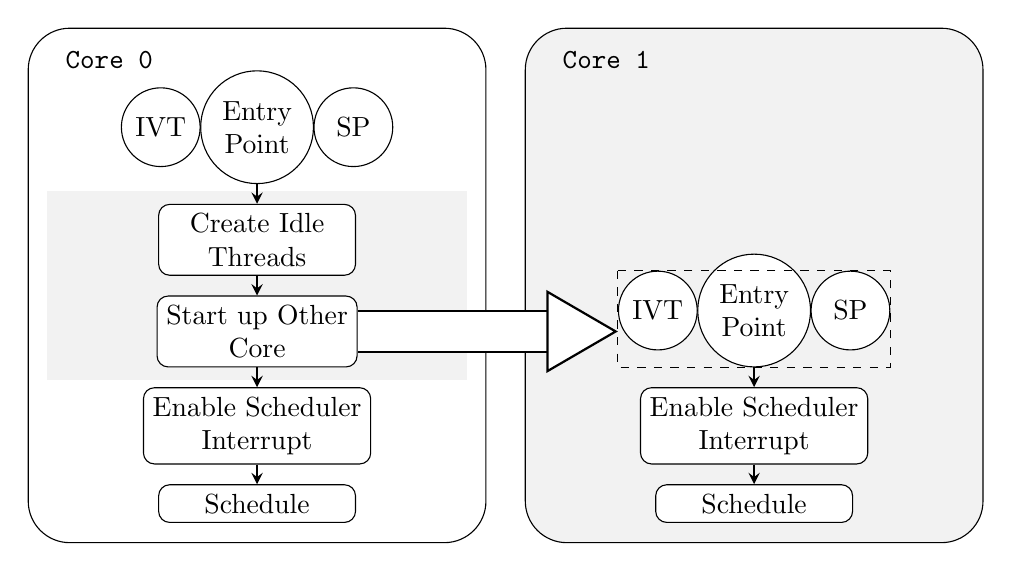
\begin{tikzpicture}  
        \tikzset{>=stealth}  
        \tikzstyle{arr} = [thick],  
        \tikzstyle{process} = [shape=rectangle, rounded corners, align=center, draw, minimum width=2.5cm, fill=white],  
        \tikzstyle{data} = [shape=circle, align=center, draw, minimum width=1cm, fill=white],  
        \coordinate (bottomend) at (\columnwidth, 0);  
        \coordinate (bottombegin) at (0, 0);  
        \coordinate (bottommid) at ($(bottomend)!0.5!(bottombegin)$);  
        \coordinate (core0end) at ($(bottommid) - (0.25, 0)$);  
        \coordinate (core1start) at ($(bottommid) + (0.25, 0)$);  
        \coordinate (core0mid) at ($(core0end)!0.5!(bottombegin)$);  
        \coordinate (core1mid) at ($(core1start)!0.5!(bottomend)$);  
   
        \node [process, anchor=south, name=schedule] at (0,0.25 -| core0mid) {Schedule};  
        \node [process, anchor=south, name=irq, yshift=0.25cm] at (schedule.north) {Enable Scheduler\\Interrupt};  
        \node [process, anchor=south, name=otherCore, yshift=0.25cm] at (irq.north) {Start up Other\\Core};  
        \node [process, anchor=south, name=idle, yshift=0.25cm] at (otherCore.north) {Create Idle\\Threads};  
   
        \node [data, anchor=south, name=ef0, yshift=0.25cm] at (idle.north) {Entry\\Point};  
        % \node [data, anchor=south, name=vt0] at ($(ef0.north -| bottombegin)!0.5!(ef0.north)$) {IVT};  
        \node [data, name=vt0, xshift=-0.5cm] at (ef0.west) {IVT};  
        % \node [data, anchor=south, name=sp0] at ($(ef0.north)!0.5!(ef0.north -| core0end)$) {SP};  
        \node [data, name=sp0, xshift=0.5cm] at (ef0.east) {SP};  
  
        % core 1  
        \node [process, anchor=south, name=schedule1] at (0,0.25 -| core1mid) {Schedule};  
        \node [process, anchor=south, name=irq1, yshift=0.25cm] at (schedule1.north) {Enable Scheduler\\Interrupt};  
  
        \node [data, anchor=south, name=ef1, yshift=0.25cm] at (irq1.north) {Entry\\Point};  
        % \node [data, anchor=south, name=vt1] at ($(ef1.north -| core1start)!0.5!(ef1.north)$) {IVT};  
        % \node [data, anchor=south, name=sp1] at ($(ef1.north)!0.5!(ef1.north -| bottomend)$) {SP}; 
        \node [data, name=vt1, xshift=-0.5cm] at (ef1.west) {IVT}; 
        \node [data, name=sp1, xshift=0.5cm] at (ef1.east) {SP};  
        \draw [dashed] (vt1.west |- vt1.north) rectangle (sp1.east |- ef1.south);   
  
        % arrows  
        \draw [arr,->] (ef0.south) -- (idle.north);  
        \draw [arr,->] (idle.south) -- (otherCore.north);  
        \draw [arr,->] (otherCore.south) -- (irq.north);  
        \draw [arr,->] (irq.south) -- (schedule.north);  
  
        \draw [arr,->] (irq1.south) -- (schedule1.north);  
        \draw [arr,->] (ef1.south) -- (irq1.north);  
        
  
        \draw [thick, double distance=0.5cm, {-Triangle[scale=0.5,fill=white]}] (otherCore.east) -- (vt1.west |- otherCore.east);  
                                                                                      
        \coordinate (topend) at ($(\columnwidth,0 |- sp0.north) + (0,0.75)$);         
        \coordinate (topbegin) at (0, 0 |- topend);                                   
        \coordinate (topmid) at ($(topend)!0.5!(topbegin)$);                          
        \coordinate (core0northeast) at ($(topmid) - (0.25, 0)$);                     
        \coordinate (core1northwest) at ($(topmid) + (0.25, 0)$);                     
                                                                                      
        \node [anchor=north west, xshift=10pt, yshift=-5pt] at (topbegin) {\texttt{Core 0}};       
        \node [anchor=north west, xshift=10pt, yshift=-5pt] at (core1northwest) {\texttt{Core 1}};  
        \begin{scope}[on background layer]                                            
            \draw [rounded corners=15pt, fill=gray!10] (topend |- 0,0) rectangle (core1northwest);  
            \draw [rounded corners=15pt] (0, 0) rectangle (core0northeast);           
            \draw [fill=gray!10, draw=gray!10] ($(idle.north -| bottombegin) + (0.25,0.15)$) rectangle ($(otherCore.south -| core0end) - (0.25,0.15)$);  
        \end{scope}                                                                   
                                                                                      
    \end{tikzpicture}                                

\fi
\centering
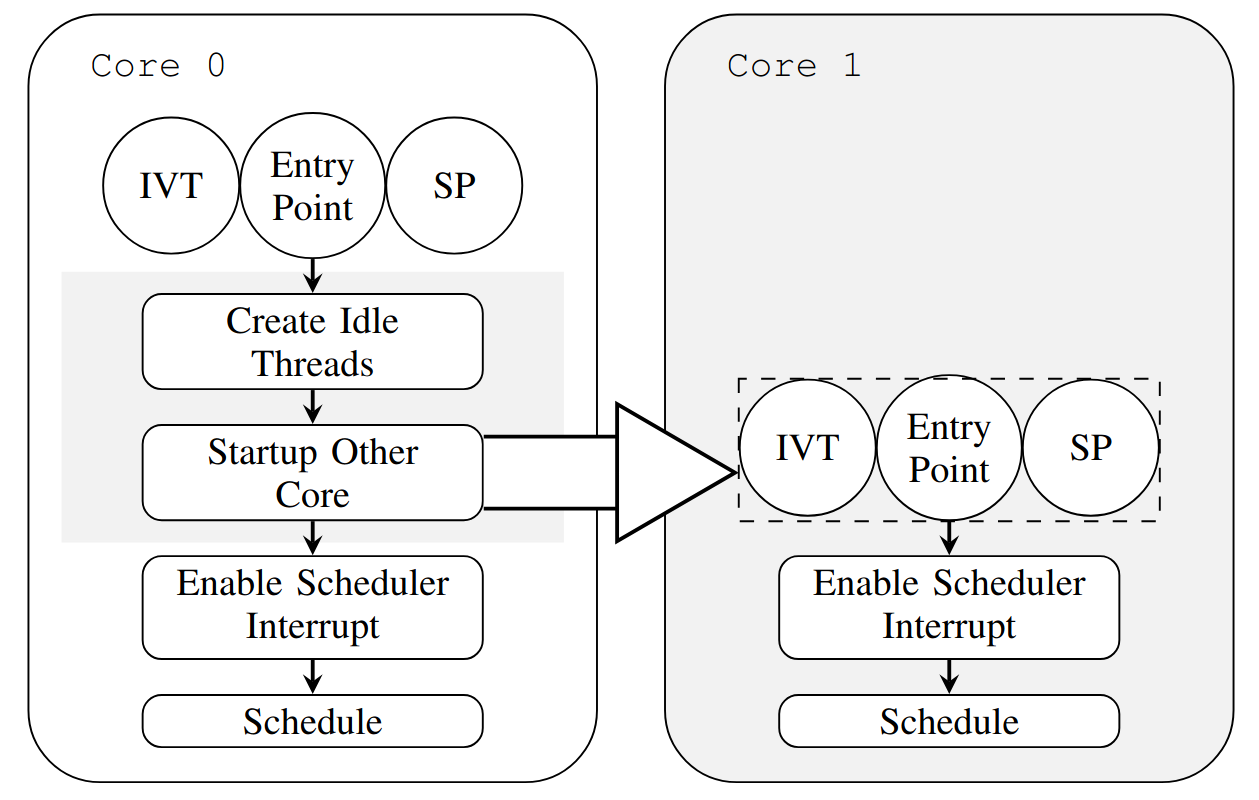
\includegraphics[width=0.95\columnwidth]{translate/figures/threading-startup-render-2.png}
     \caption{双核系统上的线程启动}
     \label{fig:startup}
 \end{figure}




\iffalse
\subsection{Idle Threads}

When a core is idle, it is prompted to enter low-power mode until the next thread is ready and waiting.
% Two alternative mechanisms are used to enter idle mode, depending on whether a system is single- or multicore. %\noteCA{``Two'' mechanisms?} 
On single-core, idle mode is entered in the scheduler exception, resulting in a lazy context switch (i.e. context is switched only when a different thread requires that). 
On multicore, however, such lazy context switching can result in race conditions, and thus idle threads are used instead.
% More in details: one idle thread is created per core during startup at the lowest priority.
% When no other thread is ready, the scheduler will execute this thread.
The idle threads execute at lowest priority and simply prompt the core to enter low-power mode until an interrupt occurs.
\fi

\subsection{全局调度方案}\label{sec:design:scheduling}


% \begin{itemize}
%     \item Two alternative designs: \textit{Global reallocation} routine (ThreadX) and \textit{Dynamic selection} (FreeRTOS, Nuttx, RT-Thread) approach
%     \begin{itemize}
%         \item 2-3 sentences each how they work on a high level
%     \end{itemize}
% \end{itemize}



% \OSname{} uses a global scheduling scheme.

% Global scheduling facilitates thread migration, where threads migrate between cores between executions.
% We chose global scheduling because it reduces context switches and priority inversions, and makes better use of the overall capacity~\cite{hardrealtime-multiprocessor-survey, brandenburg}.
% Furthermore, it avoids the thread allocation problem of partitioned scheduling, i.e., the problem of finding an optimal allocation of threads to cores.
% The main drawback of global scheduling is scalability, when the global runqueue becomes a bottleneck for context switching~\cite{EDF-RM-multiprocessor-survey}. However, this issue is negligible on MCUs --- which have a low processor count.
\OSname{} 使用全局调度方案

全局调度支持线程迁移,允许线程在执行过程中在不同核心之间动态移动。我们选择全局调度,是因为它能够有效减少上下文切换的频率,降低优先级反转的风险,并且更高效地利用整体计算资源~\cite{hardrealtime-multiprocessor-survey, brandenburg}。此外,全局调度还避免了分区调度中常见的线程分配难题,即如何为每个核心找到最优的线程分配方案。全局调度的主要缺点是其在可扩展性方面的局限性,尤其是在全局运行队列可能成为上下文切换瓶颈的情况下~\cite{EDF-RM-multiprocessor-survey}。然而,在微控制器场景中,由于处理器核心数量通常较少,这一问题的影响几乎可以忽略不计。


% \subsection{Assigning Threads to Cores}
% \label{sec:Assigning-Threads-to-Cores}
% With the single-core configuration, the thread-selection process simply reads the head of the runqueue. 
% However, on multicore, this would result in the same thread being executed on multiple cores.
% There are various approaches for selecting the next thread that a core should execute.
% We initially designed our scheduler so that it can accommodate either \textit{core reallocation} or alternatively \textit{dynamic thread selection} (see \autoref{sec:multicore-sched}). We then implemented both, before reporting on their performance on different hardware in \autoref{sec:benchmarks}.
\subsection{线程分配到核}
\label{sec:Assigning-Threads-to-Cores}
在单核配置中,线程选择过程仅需读取运行队列的头部。然而,在多核配置下,这种简单的选择方式会导致同一个线程在多个核上被执行。为了避免这种情况,我们探索了多种线程分配策略。我们最初设计的调度器能够灵活支持 \textit{核重分配} 或 \textit{动态线程选择}(参见 \autoref{sec:multicore-sched})。此后,我们不仅实现了这两种方法,还在 \autoref{sec:benchmarks} 中详细报告了它们在不同硬件平台上的性能表现。
%in our multicore effort in order to make an informed decision for our final implementation.

%  \begin{figure}[b]
%      \centering
%      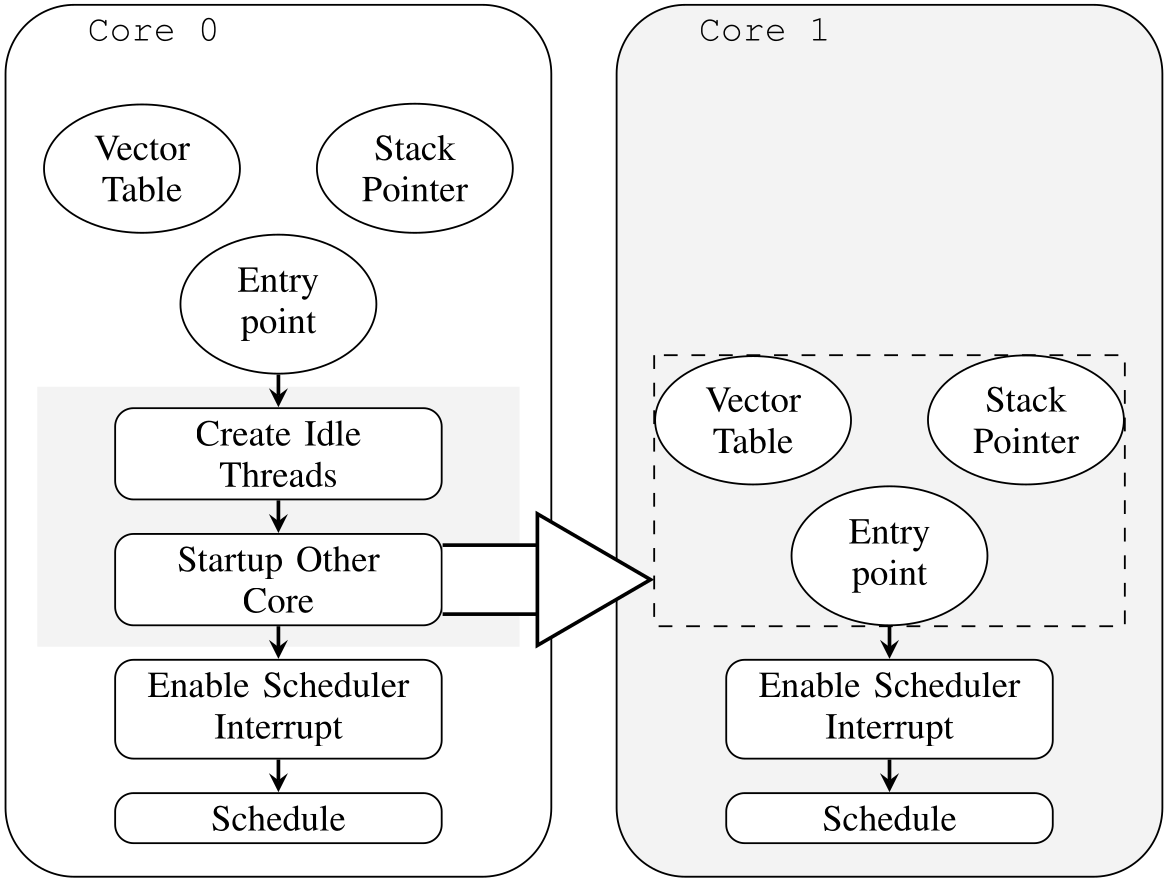
\includegraphics[width=\linewidth]{figures/threading-startup-render.png}
%      \caption{Threading startup on a dual-core system.}
%      \label{fig:startup}
%  \end{figure}

\iffalse
\subsubsection{Core Reallocation}

With this approach, a \textit{reallocation} routine maps the \textit{n} highest priority threads to the \textit{n} cores.
The allocation for each core is stored in an array that the scheduler interrupt handler reads upon invocation.
After each change in the runqueue, the \textit{reallocation} routine is executed.
It compares the previous allocation with the current highest priority threads in the runqueue, and updates the core allocation list with the goal of minimizing changes, and thus thread migration.
Based on the allocation changes, the routine returns the ID of the core where a context switch is needed.
A prominent example that follows this design is the ThreadX operating system.

\subsubsection{Dynamic Thread Selection}

In an alternative approach, implemented in FreeRTOS, NuttX, Zephyr or RT-Thread, the next thread for a core is selected directly from the runqueue by the scheduler interrupt handler upon invocation.
The thread is then removed from the runqueue to prevent it from being selected for multiple cores.
Conversely, when a running thread is preempted, it is re-added to the runqueue.
The scheduler uses the information it has readily available about thread state changes to trigger a scheduler interrupt on the specific core where a context switch is needed.
For instance, if a high-priority thread becomes ready, the scheduler interrupt is set for the core that is currently executing the lowest-priority thread.

\fi

% In an alternative approach, the scheduler selects the next thread for a core, in a dynamic fashion, upon invocation.
% The global scheduler uses the information it has readily available about changes in thread state changes, in the runqueue changes, to invoke the scheduler on the specific core where a context switch is needed.
% \noteEB{I attempted reformulation because it was difficult to parse. But somehow it is *still* difficult to parse. In particular, if there is a global scheduler, it should not sound suddenly like there are multiple schedulers...}
% The scheduler then %reads the next thread from the runqueue and 
% removes the thread from the runqueue, to prevent the same thread from being selected for multiple cores.
% Conversely, when a running thread is preempted, it is re-added to the runqueue.
% \subsection{Core Affinity Masks}

% Core affinities are a feature that allows pinning a thread so it runs on some specified core(s) only. %one or multiple specific cores. 
% This provides the user with fine-grained control over how and where threads may run. 
% % For example, core affinities can be used to bind two threads with different priorities to the same core, which will ensure that they can not run in parallel, and thus mutual exclusion between them.
% Core affinities are realized with a bitmask, where a set bit encodes that the thread can run on the core with this index. 
% The scheduler uses this information when selecting the core on which a thread should run.

\subsection{核亲和性掩码}

核亲和性是一种特性,允许将线程固定到特定的核上运行。这为用户提供了对线程运行位置和方式的精细控制。

核亲和性通过位掩码实现,其中设置的位表示线程可以在该索引对应的核上运行。调度器在选择线程应运行的核时会使用这些信息

% \subsection{Dynamic Priorities and Priority Inheritance}

% Thread priorities in \OSname{} can be changed dynamically at runtime for all active threads.
% A change in priority may result in a context switch if a running thread's priority is decreased or if a waiting thread's one increased.
% Furthermore, dynamic priorities facilitate priority inheritance for mutexes.
% If a higher-priority thread is blocked on a mutex that is currently owned by a lower-priority thread, the owning thread inherits the higher priority of the waiting thread.
% This prevents the owner from being preempted by other lower-priority threads 
% and thus helps avoid priority inversions caused by indirect blocking.

\subsection{动态优先级与优先级继承}

在 \OSname{} 中,所有活动线程的优先级都可以在运行时动态调整。如果运行中的线程优先级被降低,或者等待中的线程优先级被提高,这可能会触发上下文切换。此外,动态优先级还支持互斥锁的优先级继承。当一个高优先级线程因等待一个当前由低优先级线程持有的互斥锁而阻塞时,持有互斥锁的线程将继承等待线程的较高优先级。这可以防止持有者被其他低优先级线程抢占,从而有助于避免由间接阻塞引起的优先级反转问题。

% \subsection{Synchronization in the Scheduler\label{sec:design:sync}}

% \OSname{} implements mutual exclusion in the kernel through a global critical section, effectively resulting in a \textit{Big Lock} design.
% Thus, there is no concurrency in the kernel, which is tolerable given that such operations in \OSname{} are short.
% It ensures correctness, prevents data races and deadlocks, and simplifies operations that involve multiple data structures, such as the runqueue and Thread Control Blocks (TCBs), because no individual locking is needed.
% On single-core systems, it is sufficient to mask all interrupts to create a critical section.
% In multicore systems, an additional global spinlock is required to ensure that even threads on other cores cannot enter another critical section. 

\subsection{调度器中的同步\label{sec:design:sync}}

\OSname{} 通过全局临界区在内核中实现互斥,这实际上形成了一种 \textit{大锁} 设计。
因此,在内核中不存在并发问题,鉴于 \OSname{} 中此类操作的持续时间较短,这种设计是可以接受的。
它确保了操作的正确性,防止了数据竞争和死锁,并且简化了涉及多个数据结构的操作,例如运行队列和线程控制块(TCBs),因为无需单独锁定。
在单核系统中,屏蔽所有中断就足以创建一个临界区。
在多核系统中,需要额外的全局自旋锁来确保其他核心上的线程也无法进入另一个临界区。

% \subsection{Combining Scheduled Threads \& Async Rust Tasks}\label{sec:design:async}

% \OSname{} uses async code based on \emph{Embassy}~\cite{embassy} for system initialization and in the HAL.  
% There is always a system executor for async tasks. 
% Using the preemptive scheduler --- and thus threading --- is optional. 
% If the scheduler is not used, the system executor will run in interrupt context. 
% If the scheduler is used, the system executor executes in a thread. 
% Additional executors can be started in other threads. 
% When all tasks on an executor are pending, the owning thread is suspended. 
% Threads can block on async functions and wait for async resources from an executor.
% Thus, the gap is bridged between the scheduler, async Rust, future-based concurrency, and asynchronous I/O.

\subsection{调度线程与异步 Rust 任务结合}\label{sec:design:async}

\OSname{} 使用基于 \emph{Embassy}~\cite{embassy} 的异步代码进行系统初始化和硬件抽象层(HAL)的实现。
系统中始终存在一个用于执行异步任务的系统执行器.
使用抢占式调度器以及由此产生的线程是可选的。如果未使用调度器,系统执行器将在中断上下文中运行。如果使用了调度器,系统执行器则会在一个线程中执行。额外的执行器可以在其他线程中启动。当某个执行器上的所有任务都处于挂起状态时,拥有该执行器的线程将被挂起。线程可以阻塞在异步函数上,并等待来自执行器的异步资源。
因此,\OSname{} 在调度器、异步Rust、基于future的并发以及异步I/O之间架起了桥梁。




% 
% DRAFT THAT FIRST: Goals (and non-goals) in conjunction with benchmarks planned
% (with starting point: single-core scheduler is like RIOT-rs scheduler)


% - discussion of scheduler variants:
%    - mentioned that we face crossroad/ two avenues; shortly discuss them
%    - we tested them on two platforms; compare in one benchmark, max two
%    - reduced
%    - "present thesis in two minutes"
%    - describe all feature

\section{\OSname{} 调度器实现}

% \begin{itemize}
% \item Supported multicore platforms: RP2040, ESP32-S3, (multicore RISC-V is WIP)
% \end{itemize}

% As of this writing, \OSname{} supports multicore scheduling on three popular hardware platforms/architectures: the RP2040 and RP2350 (dual-core ARM Cortex-M0+/ dual-core ARM Cortex-M33 resp.) and the \espsthree{} (dual-core Xtensa LX7). RISC-V multicore scheduling support in \OSname{} is currently a work in progress. %As our approach is portable by design, we expect RISC-V multicore scheduling support (e.g. on the Raspberry Pi Pico2) to be available soon. In the meantime, RISC-V is supported in single-core scheduling mode only. %and only on the ESP32 family for the time being. 

% The RP2040, RP2350, and the \espsthree{} are well supported in the Rust ecosystem: the former through the Embedded-Rust working group and the \verb|rp-rs| project, the latter directly by Espressif through the \verb|esp-hal| project.
% \OSname{} leverages this support in its implementation.
截至本文撰写之时,\OSname{} 已在三种主流的硬件平台/架构上实现了多核调度功能:RP2040 和 RP2350(分别为双核 ARM Cortex-M0+/ 双核 ARM Cortex-M33)以及 \espsthree{}(双核 Xtensa LX7)。目前,\OSname{} 对 RISC-V 的多核调度支持仍在开发中。%鉴于我们的方法在设计上具有可移植性,我们预计 RISC-V 的多核调度支持(例如在 Raspberry Pi Pico2 上)将很快推出。与此同时,RISC-V 仅支持单核调度模式。%并且目前仅在 ESP32 系列上支持。

RP2040、RP2350 和 \espsthree{} 在 Rust 生态中得到了良好的支持:前者通过 Embedded-Rust 工作组和 \verb|rp-rs| 项目获得支持,后者则通过 Espressif 的 \verb|esp-hal| 项目直接获得支持。
\OSname{} 在其实现中充分利用了这些支持。

% , and in the next sections we focus on describing \OSname{} multicore scheduling support for these different architectures/boards.

\subsection{硬件抽象}

% \begin{itemize}
%     \item Impact of Rust: traits \& generics; leverage ecosystem (Embassy, esp-hal)
% \end{itemize}

% One of the main objectives of our work is clear hardware abstraction and the reduction of platform-specific code.
% Adding support for another chip should be minimal effort, particularly when there is already chip support in the ecosystem.
我们工作的主要目标之一是实现清晰的硬件抽象以及减少特定平台的代码。当生态中已经存在对某个芯片的支持时,增加对该芯片的支持应当是一项轻而易举的任务。
% that can be leveraged.
% \pagebreak
% In \OSname{}, hardware abstraction occurs at two levels:

% \textit{CPU architecture abstraction ---} At this layer, the scheduler logic for a CPU architecture, e.g., Cortex-M, is implemented. 
% It involves all architecture-specific code to set up a thread stack, configure the exception used to trigger the scheduler, and the actual context-switching logic. 
    
% \textit{Chip-level abstraction ---} The platform-specific logic for SMP is implemented at this layer.
%     % Concretely, an implementation must specify the number of available cores and a method to read out the current core identifier. 
%     For multicore scheduling, two mechanisms are required,
%     \begin{enumerate*}[label=(\roman*)]
%     \item for starting up the other core(s), and 
%     \item for invoking the scheduler on a specific core
%     \end{enumerate*}. 
%     % The latter is needed because, on the above architectural layer, a scheduler invocation only targets the scheduler on the current core. 
%     % Indeed, \OSname{} scheduling logic requires that the scheduler of all cores can be triggered directly, because logic running on one core can affect the state of a thread that is running (or should be running) on another core.
% %\end{itemize}

% \OSname{} takes advantage of the Rust type system, by specifying the above abstractions as \emph{traits}~\cite{rust-book_traits}.
在 \OSname{} 中,硬件抽象发生在两个层面:

\textit{CPU 架构抽象 ——} 在这一层,实现了针对特定 CPU 架构(例如 Cortex-M)的调度器逻辑。它涵盖了设置线程栈、配置触发调度器的异常以及实际的上下文切换逻辑等所有与架构相关的代码。

\textit{芯片级抽象 ——} 在这一层,实现了特定平台的对称多处理(SMP)逻辑。

对于多核调度,需要两种机制:
\begin{enumerate}[label=(\roman*)]
    \item 用于启动其他核心(或多个核心);
    \item 用于在特定核心上调用调度器。
\end{enumerate}

\OSname{} 利用了 Rust 的类型系统,通过将上述抽象定义为 \emph{特性}(traits)~\cite{rust-book_traits} 来实现。
% that are then implemented by each platform.
% Compared to the alternative practice of simply duplicating function signatures for every platform, which is common, e.g., in hardware abstraction layers programmed in C, this design is more concise and ergonomic.
% Adding support for another platform in the scheduler only requires two traits -- one per layer -- to be implemented.
% As a result, the corresponding chip-level SMP implementations in \OSname{} are only 70 lines of Code (LOC) for the RP2040 and 66~LOC for the \espsthree{}.
在调度器中为另一个平台添加支持,仅需实现两个特性——每个层面各一个。
因此,在 \OSname{} 中,RP2040 的芯片级对称多处理(SMP)实现仅有 70 行代码,而 \espsthree{} 的实现则为 66 行代码。

\subsection{特定平台的调度逻辑}

% \noindent \textit{On the RP2040/RP2350 ---} The chip implements (in hardware) two FIFO queues between the physical cores, which are utilized by \OSname{} during startup and for scheduler invocations.
% During startup, Core 1 remains in sleep mode until it receives the vector table, stack pointer, and entry function through the FIFO queue, based on a fixed protocol.
% After startup, the FIFO queue is used to invoke the scheduler on the other core. 
% A received message will trigger an interrupt, where the handler will set the local scheduler exception.
\noindent \textit{在 RP2040/RP2350 上 ——} RP2040/RP2350 芯片在硬件层面实现了两个 FIFO 队列,用于连接两个物理核心。这些队列在 \OSname{} 的启动过程和调度器调用中发挥关键作用。在启动阶段,核心 1 保持睡眠模式,直到通过 FIFO 队列接收到向量表、栈指针和入口函数,这一过程遵循一个固定的协议。启动完成后,FIFO 队列用于在另一个核心上调用调度器。接收到的消息将触发一个中断,中断处理程序会设置本地调度器异常,从而启动调度过程。
% \noteEB{is message passing between threads etc; something that should be described/characterized at some level, before it pops up here? Should Fig. 1 include a FIFO on each core?}
% \noteEF{This specific section here concerns message passing between \textbf{Cores}, which is implemented in Hardware, and only on the RP2040. The ESP32-S3 doesn't implement such FIFO queues. Message passing between threads is possible through software channel, but I think that's othogonal to this section, and probably belongs into section \ref{sec:user-guide}?}

% \noindent \textit{On the ESP32-S3 ---} The chip does not implement any inter-processor communication channel.
% Instead, two different software-triggered CPU interrupts are used to invoke a scheduler on each core, respectively.
% Startup of the second core on the \espsthree{} is implemented by writing the address of the entry function into the boot address of Core 1, then resetting and unstalling the core.
% The entry function sets up the vector table address and the stack pointer for this core, and then runs our threading startup logic.

\noindent \textit{在 ESP32-S3 上 ——} 该芯片未实现任何处理器间通信通道。相反,它通过触发两个不同的软件中断来分别在每个核心上调用调度器。在 \espsthree{} 上启动第二个核的启动是通过将入口函数的地址写入核心 1 的启动地址,然后重置并解除该核心的停机状态来实现的。入口函数会设置该核的向量表地址和栈指针,随后运行我们的线程启动逻辑。

\subsection{中断处理}

% On the RP2040/RP2350, each core is equipped with its own ARM Nested Vectored Interrupt
% Controller (NVIC). 
% On the \espsthree{}, each core has its own configurable interrupt matrix. 
% On both chips, nested interrupts are supported, so that a lower-priority interrupt can be preempted by a higher-priority one.
% External interrupts are routed to both cores,
% but only enabled on one core for handling, as described below.
在 RP2040/RP2350 上,每个核心都配备了各自的 ARM 嵌套向量中断控制器(NVIC)。
在 \espsthree{} 上,每个核心都有其可配置的中断矩阵。
在两种芯片上,都支持嵌套中断,使得低优先级的中断可以被高优先级的中断抢占。
外部中断被路由到两个核心,但仅在一个核心上启用以进行处理,具体如下所述。

% During startup, peripherals are initialized either in interrupt mode on Core 0 before threading is started, or by one high-priority thread. % whose core affinity can optionally be set.
% This initialization configures and enables the required interrupts on the core it executes on, which will then be the core that handles the related interrupts.

% Still, both cores share the same interrupt vector table, so it is also possible to manually mask and unmask interrupts on individual cores to configure where an interrupt should be handled.
在启动期间,外设初始化要么在核心 0 上以中断模式进行,且在启动线程之前完成,要么由一个高优先级线程完成。% 其核心亲和性可以可选地设置。
这种初始化会在其执行的核心上配置并启用所需的中断,而该核心随后将负责处理相关的中断。

尽管如此,两个核心共享同一个中断向量表,因此也可以手动在各个核心上屏蔽和解除屏蔽中断,以配置中断的处理位置。

\subsection{调度器中的同步}

% The scheduler is implemented through a single structure that contains the runqueue, TCBs, and other scheduling data, and implements all scheduling logic.
% This structure is protected by a wrapper type that ensures that all accesses to the scheduler are executed inside a critical section and that no reference to the scheduler can be obtained outside of it.
调度器通过一个单一结构实现,该结构包含运行队列、线程控制块(TCBs)以及其他调度数据,并实现了所有调度逻辑。
该结构被一个包装类型保护,确保所有对调度器的访问都在临界区中执行,并且无法在临界区之外获得对调度器的引用。
% Such access is realized in Rust closures~\cite{rust-book_closures},.
% that are provided with an immutable or mutable reference to the scheduler structure as input.
% The Rust compiler prevents the reference from being moved outside this closure in any way, thus access is only possible for the duration of the closure and therefore only while inside the critical section.

\iffalse
\subsection{Lock Guards}

Lock guards are common design pattern for synchronization primitives and mutual exclusion in Rust.
In case of \OSname{}, lock guards are used in both the \verb|critical-section| crate~\cite{critical-section} that \OSname{} is using, as well as \OSname{}'s own mutex implementation.
% ~\noteEB{Link/ref to crate? And: it struck me that some readers might not know what a "crate" is. (i) what doc should we cite on crates? (ii) where should we "introduce" the notion of crate? I get the feeling "crate" should be hinted at way before this stage. Maybe in section 2, e.g. mention that we aim to "take full advantage of Rust specificity beyond memory safety, for instance the crate system, and trait zero-cost abstractions"?}
The implementation takes advantage of Rust's ownership concepts and scoping rules for ergonomic and fail-safe lock usage. The life time of a lock guard corresponds to the time a lock is held.
On one hand, lock guards ensure that an acquired lock or critical section is always released again, even in case of code panics. On the other hand, lock guards facilitate access to the protected data – in Rust, synchronization primitives like mutexes typically own the data they protect. %\noteKS { @Elena please double check this is not cutting too much}
\fi
\iffalse 
where each variable has exactly one owner, which may be, for example, the function it is declared in.
If the variable goes out of scope, e.g., because the function returns, the variable is destructed and its memory freed.
However, before doing so, the destructor will call a \verb|drop| function first on the type itself, and then recursively on all its inner types. 
This \verb|drop| function can be implemented by the crate that defines the type, to add logic that should run just before the type is destructed.

In the case of lock guards, the \verb|drop| function is implemented to release the associated lock, and more precisely, this is also \textit{the only way to release a lock}.
If the lock should be released before the guard would usually go out of scope, it can be dropped manually, after which the guard is no longer accessible.
Thus, there is no way the protected inner data is accidentally accessed after the lock was already released.


\noteEF{Koen noted that this section may not be relevant/ interesting to the user. Purpose was to show how Rust impact the implementation of synchronization primitives and the gain from that. But if we're short on space, maybe remove this section?}
\noteEB{Let's first try to make it shorter, and tighten the rest too. Remove in last resort. Rust specifics = good}

% - mention stuff that specific to embedded Rust in that context
%    - discuss challenged and opportunities that come from Rust
\fi
\section{使用 \OSname{} 多核的微基准测试}
\label{sec:benchmarks}


% We next evaluate the performance of \OSname{} on popular hardware. We published our benchmark code in~\cite{ariel-benchmarks}. 

% The \textbf{dual-core MCUs} we used are:
% \begin{enumerate*}[label=(\roman*)]
% \item Espressif \espsthree{} with dual Xtensa LX7 at 240 MHz, and 
% \item RP2040/RP2350 with dual Cortex-M0+/M33 at 133/150 MHz.
% \end{enumerate*}


% The \textbf{single-core boards} we used for comparison are:
% \begin{enumerate*}[label=(\roman*)]
% \item a Nordic nRF52840 with a Cortex-M4 at 64 MHz, and 
% \item an Espressif \espcthree{} with a RISC-V RV32IMC at 160 MHz.
% \end{enumerate*}
接下来,我们在主流的硬件平台上评估了 \OSname{} 的性能。我们的基准测试代码已发布在~\cite{ariel-benchmarks}。

我们使用的\textbf{双核 MCU}包括:
\begin{enumerate}[label=(\roman*)]
\item Espressif \espsthree{},配备双核 Xtensa LX7,主频 240 MHz;
\item RP2040/RP2350,配备双核 Cortex-M0+/M33,主频分别为 133 MHz 和 150 MHz。
\end{enumerate}

我们用于对比的\textbf{单核开发板}包括:
\begin{enumerate}[label=(\roman*)]
\item Nordic nRF52840,配备 Cortex-M4,主频 64 MHz;
\item Espressif \espcthree{},配备 RISC-V RV32IMC,主频 160 MHz。
\end{enumerate}
%\footnote{The benchmarks are available at \url{https://github.com/elenaf9/RIOT-rs-benchmarks}. The used commit revision is \textit{TODO}.} that compare the scheduler performance, quantify the speedup, and ...(\textit{TBC}).
\iffalse
We measured performance on the following popular boards, commercially available off-the-shelf: 
\begin{itemize}
    \item Nordic nRF52840: Arm Cortex\nobreakdash-M4, single-core, 64 MHz, 256 KB RAM, 1 MB Flash memory;
    \item Espressif \espcthree{}: RISC\nobreakdash-V RV32IMC, single-core, 160 MHz, 400 KB SRAM, 4 MB Flash memory;
    \item Espressif \espsthree{}: Xtensa LX7, dual-core, 240 MHz, 8 MB RAM, 16 MB Flash memory;
    \item RaspberryPi Pico: Arm Cortex\nobreakdash-M0+, dual-core,  133 MHz, 264 KB SRAM, 2 MB Flash memory.
\end{itemize}
\fi

% On Xtensa and Cortex-M, the performance is measured in ticks.
在 Xtensa 和 Cortex-M 架构上,性能是通过时钟周期(ticks)来衡量的。
\iffalse
\begin{itemize}
    \item Cortex-M: SysTick timer with the processor clock as the clock source
    \item Xtensa: CCOUNT cycle count registers
    % \item RISC-V: \noteEF{Unfortunately we can't measure the performance in ticks on the ESP32-C3 or ESP32-C6, because the \textit{mcycle} register isn't implemented on RV32IMC... Instead we have to use the system timer at 16Mhz... do we even need benchmark data for a second single-core board?}
\end{itemize}
\fi
% On the RISC-V-based \espcthree{}, we instead use the system timer, which runs at 16 MHz.
% The measurements we present are the average of 1000 runs.
在基于 RISC-V 的 \espcthree{} 上,我们使用系统定时器进行测量,该定时器运行频率为 16 MHz。
我们所展示的测量结果是 1000 次运行的平均值。
%, at 10\%  of the processor clock speed.
%Each benchmark consists of one or multiple threads, configured at the lowest priority, of which one executes the benchmark function.
% Results were deemed valid only if no timer/counter wrap-around and no thread migration of the benchmark-thread happened.% wrap, and the benchmarking thread didn’t migrate between cores. 



\subsection{比较多核调度器的差异}

%We compare the scheduler performance of the two global multicore scheduler implementations discussed in \ref{sec:design:scheduling} on dual-core platforms with each other, and against the baseline RIOT-rs scheduler. For this, a simple benchmark was implemented where two pairs of threads alternate in waking each other and then suspending their own execution by setting and waiting for thread flags. Hence, the benchmark largely consists of context switches.
% \autoref{fig:flags} depicts micro-benchmarks in which four threads, grouped into pairs, alternate in waking each other up and then suspending their own execution. % by setting and waiting for thread flags (hence the cost of context switches dominates here). 
% We compare the performance of different variants of the scheduler: (i) the \emph{single-core} variant described in \autoref{sec:single-core}, (ii) a multicore variant using \emph{core reallocation}, and (iii) a multicore variant using \emph{dynamic thread selection} as mentioned in \autoref{sec:Assigning-Threads-to-Cores}. 

\autoref{fig:flags} 展示了一个微基准测试,其中四条线程被分为两组,交替唤醒对方并挂起自己的执行。% 通过设置和等待线程标志(因此上下文切换的成本在这里占主导地位)。
我们比较了不同调度器变体的性能:(i) 在 \autoref{sec:single-core} 中描述的 \emph{单核} 变体,(ii) 使用 \emph{核重分配} 的多核变体,以及 (iii) 在 \autoref{sec:Assigning-Threads-to-Cores} 中提到的使用 \emph{动态线程选择} 的多核变体。


\pgfplotstableread[col sep=comma,]{translate/data/flags_dual-core_espressif-esp32-s3-devkitc-1.csv}\flagsdualesp{}
\pgfplotstableread[col sep=comma,]{translate/data/flags_dual-core_rpi-pico.csv}\flagsdualpico{}
\pgfplotstableread[col sep=comma,]{translate/data/flags_dual-core_rpi-pico2.csv}\flagsdualpicotwo{}
\begin{figure}[t!]
     \begin{subfigure}[t]{0.49\columnwidth}
     \begin{tikzpicture}
         {
            \begin{axis}[
            ybar,
            ourybarstyle,
            bar width=8pt,
            enlarge x limits=0.2,
            height=4cm, width=\textwidth,
            ylabel={Ticks},
            ytick distance=1000,
            symbolic x coords={{Single Core},{Multicore (Reallocation)},{Multicore (Dynamic)}},
            xticklabels={{Single Core},{Multicore\\(Reallocation)},{Multicore\\(Dynamic)}},
            nodes near coords style={font=\small, black, rotate=70, anchor=south east, yshift=-6pt, xshift=+27pt},
            xticklabel style={font=\small, rotate=45, anchor=east, align=right},
        ]
      \addplot table [y index=1]{\flagsdualpico};
      \addplot table [y index=1]{\flagsdualpicotwo};
    \end{axis}}
    \end{tikzpicture}
    \caption{RP2040/RP2350 (blue/purple)\label{fig:flags_rp2040}}
     \end{subfigure}
     \begin{subfigure}[t]{0.49\columnwidth}
     \begin{tikzpicture}
         {
            \begin{axis}[
            ybar,
            ourybarstyle,
            bar width=15pt,
            enlarge x limits=0.2,
            height=4cm, width=\textwidth,
            ylabel={Ticks},
            ytick distance=1000,
            symbolic x coords= {{Single Core},{Multicore (Reallocation)},{Multicore (Dynamic)}},
            xticklabels={{Single Core},{Multicore\\(Reallocation)},{Multicore\\(Dynamic)}},
            nodes near coords style={font=\small, black, rotate=45, anchor=south west, xshift=-2pt},
            xticklabel style={font=\small, rotate=45, anchor=east, align=right},
        ]
      \addplot table [y index=1]{\flagsdualesp};
    \end{axis}}
    \end{tikzpicture}
    \caption{ESP32-S3 (dual Xtensa LX7)\label{fig:flags_esp32s3}}
    \end{subfigure}
    \caption{两种多核调度器设计的上下文切换性能与单核配置的对比 \label{fig:flags}}
\end{figure}

% The results show that \textit{dynamic} outperforms \textit{reallocation} on all the multicore microcontrollers we tested.

% The results show that \textit{dynamic} outperforms \textit{reallocation} on both microcontrollers we tested. 
% The relatively more complex \textit{reallocation} routine, executed after each thread state change, takes a toll. 
% We notice a degradation of the performance of \textit{reallocation} versus single-core on RP2040, whereas speedups are observed on \espsthree{}. %This can be explained by different degrees of parallelization on the two platforms.

结果表明,在我们测试的所有多核微控制器上,动态分配优于重新分配。相对复杂的重新分配例程在每次线程状态变化后执行,会带来一定的代价。

\iffalse
\begin{enumerate}
    \item The \textit{Dynamic} approach outperforms the \textit{Reallocation} on both platforms.
    \item On the RP2040, no significant speedup was achieved through the multicore configuration, and even a degradation in case of the \textit{Dynamic} approach. On the \espsthree{}, the speedup is a factor of 1.3 in the \textit{Reallocation} approach and 1.5 for the \textit{Dynamic} one.
\end{enumerate}
\fi
%(1) is likely due to the complexity of the \textit{reallocation} routine, which is executed after each thread state change. The findings in (2) can be explained by different degrees of parallelization on the two platforms.
%As discussed in \autoref{sec:design:sync}, \OSname{} applies mutual exclusion to the whole kernel, and thus %no parallelization in the scheduler is possible.
% The benchmark largely consists of scheduler operations. Thus, mutual exclusion in the scheduler forces mostly sequential execution on the RP2040.
% In contrast, on the \espsthree{}, parallelization happens differently in hardware, forcing sequential execution less often. %however, 
% Furthermore, one benchmark iteration on \espsthree{} requires
% many more ticks than on the RP2040.
% Thus, \espsthree{} reaps more benefits from parallelization in this benchmark.
% %If we assume that this can be at least partly 
% %linked to a larger cost of the scheduler interrupt (and the saving and restoring of the trap frame). Thus, this larger segment that can run independently between the cores on this platform reaps more benefits from parallelization.
% In the following, we focus on the \textit{dynamic thread selection} variant for our multicore scheduling.
该基准测试主要由调度器操作构成。因此,RP2040上的调度器互斥机制导致其主要以顺序方式执行。
相比之下,在\espsthree{}上,硬件层面的并行化机制有所不同,较少强制执行顺序操作。此外,\espsthree{}上完成一次基准测试迭代所需的时钟周期远多于RP2040。因此,在此基准测试中,\espsthree{}能够从并行化中获得更多优势。
接下来,我们将重点关注多核调度中的\textit{动态线程选择}结构。
%approach, which we study further in the following.
% for our final SMP implementation. We furthermore found this approach to be the simpler and more intuitive one of the two, although additional care must be taken due to the lack of a global state. The following subsections use the \textit{dynamic} scheduler implementations for multicore.

% \iffalse
% \begin{figure}[htbp]
%      \begin{subfigure}[t]{0.49\columnwidth}
%     \centering
%          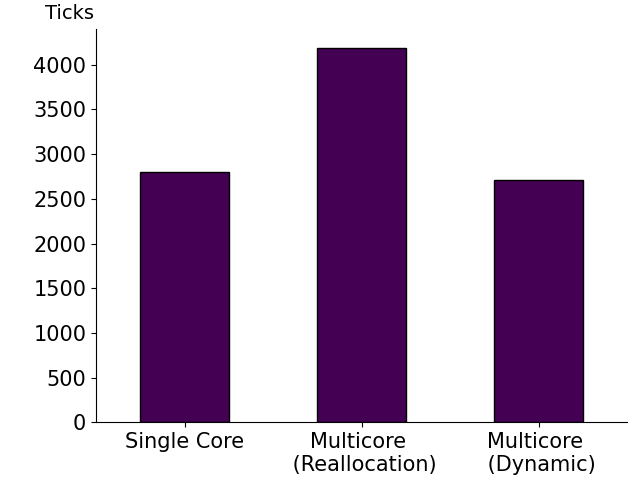
\includegraphics[width=\textwidth]{figures/flags_dual-core_rpi-pico.png}
%          \caption{RP2040 (dual Cortex-M0+)\label{fig:flags_rp2040}}
%      \end{subfigure}
%      \hfill
%      \begin{subfigure}[t]{0.49\columnwidth}
%          \centering
%          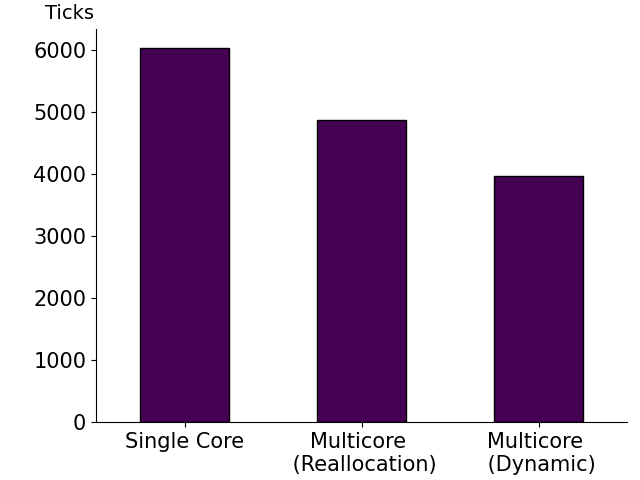
\includegraphics[width=\textwidth]{figures/flags_dual-core_espressif-esp32-s3-wroom-1.png}
%          \caption{ESP32-S3 (dual Xtensa LX7)\label{fig:flags_esp32s3}}
%      \end{subfigure}
%     \caption{Context switching performance of the two multicore scheduler designs compared with single-core configuration~.\label{fig:flags}}
% \end{figure}
% \fi
\subsection{多核调度的开销}

% We next measure
% the overhead of our multicore scheduling feature, compared to the single-core scheduler we started from in \autoref{sec:single-core}.
% For this, we focus on thread preemption, because, compared to single-core, the multicore feature adds an additional step: inserting the preempted thread back into the runqueue. %, whereas in the case of single-core this step is skipped.
% \autoref{fig:preempt} reports on micro-benchmarks performed on different single-core boards, in which a lower-priority thread sets the flag for a higher-priority thread, resulting in a context switch.

% We observe that the overhead when the multicore feature is enabled remains quite small, approx. 9.6\% on the nRF52840 and 5.3\% on the \espcthree{}. 
% Conveniently, we can therefore enable multicore by default

% in \OSname{}.

接下来,我们测量多核调度功能的开销,并将其与我们在\autoref{sec:single-core}中开始时的单核调度器进行比较。为此,我们专注于线程抢占,因为与单核相比,多核功能增加了一个额外的步骤:将被抢占的线程重新插入运行队列。%而在单核情况下,此步骤会被跳过。
\autoref{fig:preempt}报告了在不同单核开发板上进行的微基准测试结果,其中低优先级线程设置了一个标志以触发高优先级线程的运行,从而导致上下文切换。
我们观察到,启用多核功能时的开销仍然很小,在nRF52840上约为9.6%,在\espcthree{}上约为5.3%。因此,我们可以在\OSname{}中默认启用多核功能。

\pgfplotstableread[col sep=comma,]{translate/data/preempt_both_ai-c3.csv}\preemptesp{}
\pgfplotstableread[col sep=comma,]{translate/data/preempt_both_nrf52840dk.csv}\preemptnrf{}
\begin{figure}[t!]
     \begin{subfigure}[t]{0.49\columnwidth}
     \begin{tikzpicture}
         {
            \begin{axis}[
            ybar,
            ourybarstyle,
            bar width=20pt,
            enlarge x limits=0.4,
            height=4cm, width=\textwidth,
            ylabel={Ticks},
            ytick distance=200,
            symbolic x coords={{Multicore scheduler disabled},{Multicore scheduler enabled}},
            xticklabels={{disabled},{enabled}},
            nodes near coords style={font=\small, black, rotate=45, anchor=south west, xshift=-2pt},
            xticklabel style={font=\small, align=center},
        ]
      \addplot table [y index=1]{\preemptnrf};
    \end{axis}}
    \end{tikzpicture}
         \caption{nRF52840 (Cortex-M4)\label{fig:preempt_nrf52840}}
     \end{subfigure}
     \begin{subfigure}[t]{0.49\columnwidth}
     \begin{tikzpicture}
         {
            \begin{axis}[
            ybar,
            ourybarstyle,
            bar width=20pt,
            enlarge x limits=0.4,
            height=4cm, width=\textwidth,
            ylabel={Ticks},
            ytick distance=50,
            symbolic x coords={{Multicore scheduler disabled},{Multicore scheduler enabled}},
            xticklabels={{disabled},{enabled}},
            nodes near coords style={font=\small, black, rotate=45, anchor=south west, xshift=-2pt},
            xticklabel style={font=\small, align=center},
        ]
      \addplot table [y index=1]{\preemptesp};
    \end{axis}}
    \end{tikzpicture}
         \caption{ESP32-C3 (RISC-V)\label{fig:preempt_esp32c3}}
    \end{subfigure}
    \caption{在单核硬件上测量的多核调度特性开销 %when a running thread is being preempted on a single-core board.
    \label{fig:preempt}}
\end{figure}
% \iffalse
% \begin{figure}[htbp]
%      \begin{subfigure}[t]{0.24\textwidth}
%          \centering
%          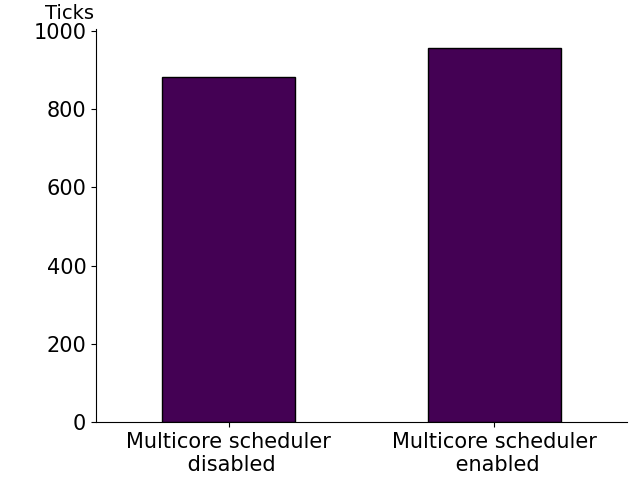
\includegraphics[width=\textwidth]{figures/preempt_both_nrf52840dk.png}
%          \caption{nRF52840 (Cortex-M4)\label{fig:preempt_nrf52840}}
%      \end{subfigure}
%      \hfill
%      \begin{subfigure}[t]{0.24\textwidth}
%          \centering
%          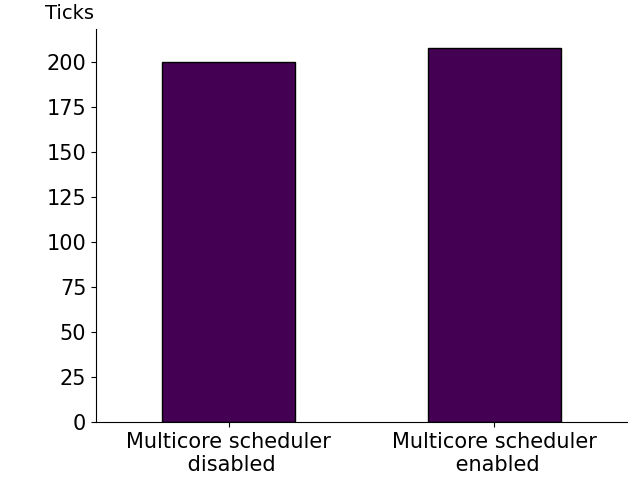
\includegraphics[width=\textwidth]{figures/preempt_both_ai-c3.png}
%          \caption{ESP32-C3 (RISC-V)\label{fig:preempt_esp32c3}}
%      \end{subfigure}
%     \caption{Overhead of the multicore scheduling feature when a running thread is being preempted.\label{fig:preempt}}
% \end{figure}
% \fi  

\subsection{计算密集型任务的加速}

\pgfplotstableread[col sep=comma,]{translate/data/matrix-mult_speedup_espressif-esp32-s3-devkitc-1.csv}\matrixesp{}
\pgfplotstableread[col sep=comma,]{translate/data/matrix-mult_speedup_rpi-pico.csv}\matrixpico{}
\pgfplotstableread[col sep=comma,]{translate/data/matrix-mult_speedup_rpi-pico2.csv}\matrixpicotwo{}
\begin{figure}[t]  
     \begin{subfigure}{0.49\columnwidth}
     \begin{tikzpicture}                                                   
         {
            \begin{axis}[                  
            ourlinestyle,              
            height=4cm, width=\textwidth,  
            ylabel={Relative speedup},     
            ytick distance=0.5,         
            tension=0.1,                
        ]                               
        \addplot+[myTeal, mark options={fill=myTeal}] table [x=0, y=speedup] {\matrixpico};                    
        \addplot+[myEggplant, mark options={fill=myEggplant}] table [x=0, y=speedup] {\matrixpicotwo};
    \end{axis}}                           
    \end{tikzpicture}      
     \caption{RP2040/RP2350 (blue/purple)\label{fig:matrix-mult_rp2040}}
     \end{subfigure}                                                   
     \begin{subfigure}{0.49\columnwidth}                                                                            
     \begin{tikzpicture}                                                                                                          
         {                                                                                                              
            \begin{axis}[                                                                                    
            ourlinestyle,                                                                             
            height=4cm, width=\textwidth,
            ylabel={Relative speedup},
            ytick distance=0.5,
        ]
        \addplot+[myTeal, mark options={fill=myTeal}] table [x=0, y=speedup] {\matrixesp};
    \end{axis}}             
    \end{tikzpicture}
         \caption{ESP32-S3 (dual Xtensa LX7)\label{fig:matrix-mult_esp32s3}}
    \end{subfigure}                                                             
    \caption{\(N\times N\) 矩阵的乘积, \(N\in\{10, 20, ...,  80\}\)\label{fig:matrix-mult}}
\end{figure}  
% We next benchmark 
% $N\times N$ matrix multiplication, with and without the multicore feature. 
% In the single-core configuration, the two computations are executed sequentially.
% For multicore, the tasks are distributed to two threads that are scheduled in parallel.
% We observe in Fig.~\ref{fig:matrix-mult} that when $N$ is small, IPC overhead dominates parallelization gains. When $N$ grows larger, we observe a performance gain tending towards 2x.
% We also notice that performance gains are not strictly linear. This is subject for further investigation --- it might be due to MCU-specific memory subsystem characteristics. %, subject to further investigation. 
% For example, on the RP2040, both cores compete for a shared memory bus~\cite{pico-mem-layout}.
接下来,我们分别在启用和未启用多核功能的情况下, 进行了 $N\times N$ 矩阵乘法的基准测试。在单核配置中,两次计算是顺序执行的。对于多核配置,任务被分配到两个线程中,并且这两个线程是并行调度的。
从图~\ref{fig:matrix-mult}中我们可以观察到,当 N 较小时,IPC(进程间通信)开销主导了并行化的收益。而当 N 增大时,我们观察到性能提升逐渐趋于 2 倍。我们还注意到性能提升并非严格线性增长。这有待进一步研究——它可能是由于 MCU(微控制器)特定的存储子系统特性所导致的。例如,在 RP2040 上,两个核会竞争共享的内存总线~\cite{pico-mem-layout}。
% \noteEF{For the record: It could still be that the speedup tends towards 2x if we test larger matrix sizes, e.g. 50x50. However, we can't do that with our benchmark because the timer wraps before the computation is completed.}

\textbf{总结 ---} 通过采用全局调度方案和优先级机制,我们实现了\emph{持续工作}和\emph{实时性}特性。我们的硬件抽象提供了\emph{可移植性},并且我们通过实验测量展示了\emph{透明性}。因此,我们已经实现了我们在第~\ref{sec:goals}节中设定的目标。
% \iffalse
% \begin{figure}[b!]
%      \centering
%      \begin{subfigure}[t]{0.24\textwidth}
%          \centering
%          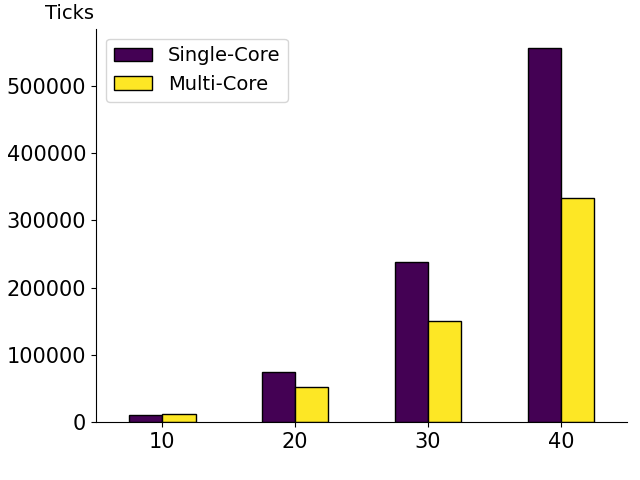
\includegraphics[width=\textwidth]{figures/matrix-mult_dual-core_rpi-pico.png}
%          \caption{RP2040\label{fig:matrix-mult_rp2040}}
%      \end{subfigure}
%      \hfill
%      \begin{subfigure}[t]{0.24\textwidth}
%          \centering
%          \includegraphics[width=\textwidth]{figures/matrix-mult_dual-core_espressif-esp32-s3-devkitc-1.png}
%          \caption{ESP32-S3\label{fig:matrix-mult_esp32s3}}
%      \end{subfigure}
%     \caption{Matrix-Multiplication performance of single- vs multicore for NxN matrices, \(N\in\{10, 20, 30, 40\}\)\label{fig:matrix-mult}}
% \end{figure}
% \fi
                             



%\textbf{Summary ---} Multicore scheduling overhead compared to a single-core scheduling variant is measurable but minor, thus the multicore variant can be the default on all platforms. In practice, parallel computation speedup with multicore scheduling is indeed substantial: we measured up to 175\% on dual core. \emph{Dynamic thread selection} outperforms other multicore variants, so we chose it as our default in \OSname{}. 
 %\noteEB{Kaspar TO DO: check the summary}
\section{Ariel 操作系统概述 %\& User Guide
}\label{sec:user-guide}

 \begin{figure}[t!]
     \centering
     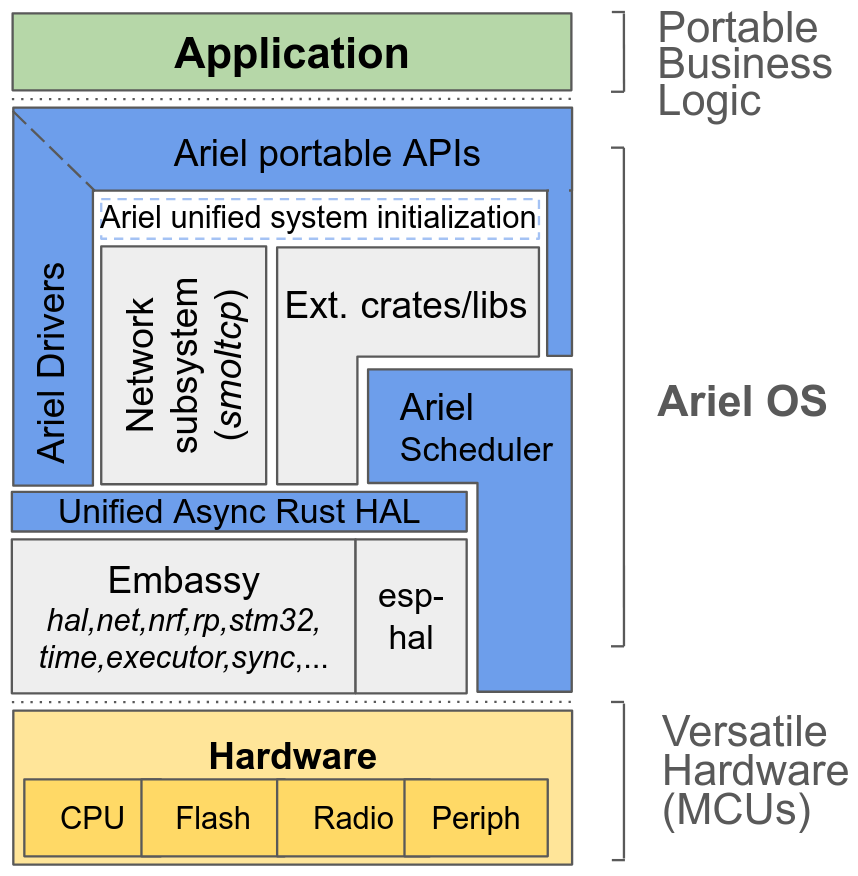
\includegraphics[width=0.7\linewidth]{translate/figures/arch-diagram-v4.png}
     \caption{\OSname{} 体系结构图%\noteCA{Ariel portable APIs also reach down to the Ariel scheduler; making it more closed and less fragmented. And this will need a color code legend.}
     }
     \label{fig:ariel-arch}
 \end{figure}
 

%\noteEB{Kaspar TO DO: choose a diagram ;)} \noteKS{I prefer EB's diagram, I tried to put in more embassy}
%Beyond its scheduler, \OSname{} aims to be a one-stop-shop for distributed computing and networked applications on heterogeneous 32-bit MCUs.
% \OSname{} is fully open-source~\cite{ariel-os-repo}. For basic hardware abstraction and async Rust programming, \OSname{} builds on top of Embassy~\cite{embassy}. Fig. \ref{fig:ariel-arch} shows how \OSname{} components (in blue) harness the ecosystem of embedded Rust (in grey).
% In particular, \OSname{} combines the following elements:
\OSname{}是完全开源的~\cite{ariel-os-repo}。对于基础硬件抽象和异步Rust编程,\OSname{}基于Embassy构建~\cite{embassy}。图\ref{fig:ariel-arch}展示了\OSname{}组件(蓝色部分)是如何利用嵌入式Rust生态系统(灰色部分)的。
具体来说,\OSname{}结合了以下元素:
%It tries to achieve that by increasing the level of abstraction, providing re-usable building blocks with usable defaults, better supporting diverse configurations in the build system, reducing boiler plate... higher level of abstraction makes high-level features possible ...
%\noteCA{… ``by providing convenient defaults for repetitive tasks of application developers''? (may be in a direction not useful for the audience, EB has opinion)}
\iffalse
\begin{itemize}
    \item Abstracting system initialization: system initialization is provided
    \item Unified peripheral APIs for application code portability: hardware access (sensor/actuator abstraction); network access (sock equivalent?). Code re-use of business logic across HW, e.g., our benchmarks code are completely HW-independent.
    \item Efficient code: automatic low-power mode exploitation; low memory footprint; zero-cost abstraction (exploiting Rust).
    \item Library OS: integration of curated set of drivers, crypto libs, network stacks. Various combinations/configs cover versatile use cases.
    \item Dependability: Rust inherent safeguards; Formal verification for critical modules (eg runqueue); 
    \item Networked: integrates IPv4 or IPv6, HTTP/TCP or CoAP/UDP network stacks over wireless/wired link layers, as well as network security standards (COSE, OSCORE, EDHOC, TLS...)
\end{itemize}
\fi

% \textbf{Versatile network stack configurations ---}
% \OSname{} integrates a network stack (\emph{embassy-net/smoltcp}~\cite{smoltcp}) combined with additional modules we provide allowing various network configurations. These configuration options include IPv4 and IPv6, HTTP/TCP and CoAP/UDP, over wireless and wired link layers, secured by open standards including COSE, OSCORE, EDHOC, TLS~\cite{tschofenig2019cyberphysical} and a curated set of libraries providing cryptographic backends.
\textbf{灵活的网络栈配置 ---}
\OSname{}集成了一个网络栈(\emph{embassy-net/smoltcp}~\cite{smoltcp}),并结合了我们提供的额外模块,支持多种网络配置。这些配置选项包括IPv4和IPv6、HTTP/TCP和CoAP/UDP,支持无线和有线链路层,并通过开放标准(包括COSE、OSCORE、EDHOC、TLS~\cite{tschofenig2019cyberphysical})以及精选的密码学后端库进行安全保护。

% \textbf{Abstracted system initialization ---}
% On MCUs, code initializing the system can be very challenging for developers. \OSname{} thus abstracts initialization, e.g., setting up
% \begin{enumerate}[label=(\roman*)]
% \item the network stack, 
% \item cryptographic material and identities, 
% \item the random number generator, 
% \item USB peripherals,
% \end{enumerate}
% etc. 
% Configuration is handled at build system level. Convenient defaults are provisioned. Boilerplate is thus minimized and high-level building blocks are provided to application logic. %\noteEB{Kaspar TODO: check/improve short version}
\textbf{抽象化的系统初始化 ---}
在微控制器(MCU)上,初始化系统的代码对开发人员来说可能极具挑战性。因此,\OSname{}对初始化过程进行了抽象化,例如设置:
\begin{enumerate}[label=(\roman*)]
\item 网络栈,
\item 密码学材料和身份,
\item 随机数生成器,
\item USB外设,
\end{enumerate}
等等。
配置在构建系统层面进行处理,并提供了方便的默认设置。这样可以最小化样板代码,同时为应用逻辑提供了高级构建模块。%\noteEB{Kaspar TODO: check/improve short version}

% \textbf{Unified peripheral APIs ---} 
% \OSname{} crafted peripheral initialization and setup (for GPIO, I2C, SPI accessing sensors/actuators) to be identical across MCU families. Thereby, application code written once can be compiled for all devices that \OSname{} supports. %Where MCU differences can not be hidden, they are made available in a way that maximizes portablility.
% This is a substantial improvement over the state of the art in embedded Rust (crates such as \emph{embedded-hal} or \emph{embedded-hal-async}) which leave out initialization, and thus lead to a jungle of initialization APIs --- and very limited application code portability. %\noteEB{Kaspar TODO: check/improve short version}

\textbf{统一的外设API ---}
\OSname{}设计了外设初始化和设置(针对GPIO、I2C、SPI访问传感器/执行器),使其在不同微控制器(MCU)系列中保持一致。因此,一次编写的应用程序代码可以编译到所有\OSname{}支持的设备上。%在无法隐藏MCU差异的地方,它们以最大化可移植性的方式提供。
这比嵌入式Rust的现有状态有了显著改进(例如\emph{embedded-hal}或\emph{embedded-hal-async}等crate),这些crate省略了初始化,从而导致了初始化API的混乱——以及非常有限的应用程序代码可移植性。%\noteEB{Kaspar TODO: check/improve short version}

% \textbf{Meta build system ---}
% The \OSname{} toolchain takes full advantage % of the large ecosystem of
% of the embedded Rust \emph{crates} ecosystem and the Rust build system \emph{Cargo}. To work around limitations w.r.t. extremely diverse modular target configurations, we wrapped Cargo in \emph{laze}~\cite{laze}, our meta-build system handling the huge matrix of software configurations on various boards.% We published the source code of \emph{laze} in~\cite{laze}.

\textbf{元构建系统 ---}
\OSname{}工具链充分利用了嵌入式Rust的\emph{crates}生态系统和Rust构建系统\emph{Cargo}。为了应对极其多样模块化的目标配置的限制,我们将Cargo封装在\emph{laze}~\cite{laze}中,这是一个元构建系统,用于处理各种开发板上庞大的软件配置矩阵。% 我们在~\cite{laze}中发布了\emph{laze}的源代码。

%With this landscape in mind, the remainder of the paper focuses primarily on the scheduler aspects.

\iffalse
In the embedded Rust ecosystem, the two interface-only crates `embedded-hal` and `embedded-hal-async` are the de-facto standard API for accessing an MCU's hardware peripherals like GPIO pins and I2C/SPI buses. While they enable GPIO/I2C/SPI peripherals to be used by e.g., drivers in an implementation agnostic way, the *initialization* and *setup* of the peripherals is intentionally left out of the traits in order to make them universally usable.
This leads to different `embedded-hal`(`-async`) implementations providing slightly or very different initialization APIs (\noteKS{reference embassy-hals, atsamd, esp-rs, ...?}
\OSname{} improves on this by providing a unified API for peripheral initialization that is designed to be identical across MCU families, allowing applications to be written once but compiled for all devices that \OSname{} supports. Where MCU differences can not be hidden, they are made available in a way that maximizes portablility. \noteKS{Mention frequency macro?}
\fi

% - present briefly \OSname{} as a whole with single core support (Basically RIOT-rs as it is/was), and claim explicitly as 
% - usage of Async Rust / Embassy?
% - library OS aspect
% - interaction with scheduler
% - add a brief architecture diagram 
%  (Basically: some kind of equivalent of https://inria.hal.science/hal-00945122/document (was for RIOT)
% \section{Conclusions}
% In this paper we introduced \OSname{}, the first embedded Rust operating system for microcontrollers supporting both single- and multicore preemptive scheduling combined with asynchronous Rust.
% We assessed experimentally how 
% a unique multicore scheduler can be the convenient default on all supported multicore platforms. 
% Still, applications 

% can opt out of multicore scheduling when parallelization is unneeded.

% \OSname{} thus enriches the set of available open source tools 
% for secure and efficient distributed computing applications involving sensors/actuators or small networked devices using 32-bit MCUs such as ARM Cortex\nobreakdash-M, RISC\nobreakdash-V, or ESP32.

\section{结论}
在本文中,我们介绍了\OSname{},这是第一个支持单核和多核抢占式调度以及异步Rust的微控制器嵌入式Rust操作系统。我们通过实验评估了在所有支持的多核平台上,独特的多核调度器如何可以作为便捷的默认选项。然而,当并行化并非必要时,应用程序可以选择退出多核调度。
因此,\OSname{}丰富了现有的开源工具集,适用于涉及传感器/执行器或使用32位微控制器(如ARM Cortex\nobreakdash-M、RISC\nobreakdash-V或ESP32)的小型网络设备的安全高效分布式计算应用。

%Researchers can use \OSname{} as common playground for experimental implementation and performance studies involving embedded Rust software on all the relevant 32-bit microcontroller architectures (ARM Cortex\nobreakdash-M, RISC\nobreakdash-V, ESP32).
%Industry users from diverse verticals can use \OSname{} to accelerate their transition from C/C++ towards safer embedded Rust, while benefiting from a high degree of hardware agility. %, ingrained by design. 
%\textbf{Code Availability ---} \OSname{} is fully open source~\cite{ariel-os-repo}.% and  maintained on a public git repository by 10+ people located in 4 countries across the European Union.

%in terms of reusing their software (business logic) on a wide variety of microcontroller architectures and commercially available off-the-shelf boards in this category.



% \bibliographystyle{translate/IEEEtran}
% \bibliography{translate/tlrefs.bib}



% 大量原本用C/C++实现的低级系统软件组件,目前正在被用Rust语言重新编写。Rust是一种相对更安全、更可靠的编程语言。然而,到目前为止,还没有用Rust编写的嵌入式操作系统支持微控制器上的多核抢占式调度。因此,本文填补了这一空白,提出了一个新的操作系统:Ariel OS。我们描述了它的设计,提供了其实现的源代码,并在主流的32位微控制器架构上进行了微基准测试,包括ARM Cortex-M、RISC-V和Espressif Xtensa。我们展示了我们的调度器如何在利用多核优势的同时,仅在单核硬件上产生极小的额外开销。正因如此,Ariel OS 为研究和行业从业者针对小型联网设备提供了一个便捷的嵌入式软件平台。


% \section{图表示例}

% \subsection{图}

% 附录中的图片示例(图~\ref{fig:appendix-translation-figure})。

% \begin{figure}
%   \centering
%   
\includegraphics[width=0.6\linewidth]{example-image-a.pdf}
%   \caption{附录中的图片示例}
%   \label{fig:appendix-translation-figure}
% \end{figure}


% \subsection{表格}

% 附录中的表格示例(表~\ref{tab:appendix-translation-table})。

% \begin{table}
%   \centering
%   \caption{附录中的表格示例}
%   \begin{tabular}{ll}
%     \toprule
%     文件名          & 描述                         \\
%     \midrule
%     thuthesis.dtx   & 模板的源文件,包括文档和注释 \\
%     thuthesis.cls   & 模板文件                     \\
%     thuthesis-*.bst & BibTeX 参考文献表样式文件    \\
%     thuthesis-*.bbx & BibLaTeX 参考文献表样式文件  \\
%     thuthesis-*.cbx & BibLaTeX 引用样式文件        \\
%     \bottomrule
%   \end{tabular}
%   \label{tab:appendix-translation-table}
% \end{table}


% \section{数学公式}

% 附录中的数学公式示例(公式\eqref{eq:appendix-translation-equation})。
% \begin{equation}
%   \frac{1}{2 \uppi \symup{i}} \int_\gamma f = \sum_{k=1}^m n(\gamma; a_k) \mathscr{R}(f; a_k)
%   \label{eq:appendix-translation-equation}
% \end{equation}


% \section{文献引用}

% 附录\cite{dupont1974bone}中的参考文献引用\cite{merkt1995rotational}示例
% \cite{dupont1974bone,merkt1995rotational}。


% \appendix

% \section{附录}

% 附录的内容。


% 书面翻译的参考文献
% 默认使用正文的参考文献样式;
% 如果使用 BibTeX,可以切换为其他兼容 natbib 的 BibTeX 样式。
% \bibliographystyle{unsrtnat}
% \bibliographystyle{IEEEtranN}

% 默认使用正文的参考文献 .bib 数据库;
% 如果使用 BibTeX,可以改为指定数据库,如 \bibliography{ref/refs}。
\printbibliography

% 书面翻译对应的原文索引
% \begin{translation-index}
%   \nocite{mellinger1996laser}
%   \nocite{bixon1996dynamics}
%   \nocite{carlson1981two}
%   \bibliographystyle{unsrtnat}
%   \printbibliography
% \end{translation-index}


\end{translation}
  % 本科生:外文资料的书面翻译
% % !TeX root = ../cyh.tex

\chapter{补充内容}

附录是与论文内容密切相关、但编入正文又影响整篇论文编排的条理和逻辑性的资料,例如某些重要的数据表格、计算程序、统计表等,是论文主体的补充内容,可根据需要设置。

附录中的图、表、数学表达式、参考文献等另行编序号,与正文分开,一律用阿拉伯数字编码,
但在数码前冠以附录的序号,例如“图~\ref{fig:appendix-figure}”,
“表~\ref{tab:appendix-table}”,“式\eqref{eq:appendix-equation}”等。


\section{插图}

% 附录中的插图示例(图~\ref{fig:appendix-figure})。

\begin{figure}
  \centering
  
\includegraphics[width=0.6\linewidth]{example-image-a.pdf}
  \caption{附录中的图片示例}
  \label{fig:appendix-figure}
\end{figure}


\section{表格}

% 附录中的表格示例(表~\ref{tab:appendix-table})。

\begin{table}
  \centering
  \caption{附录中的表格示例}
  \begin{tabular}{ll}
    \toprule
    文件名          & 描述                         \\
    \midrule
    thuthesis.dtx   & 模板的源文件,包括文档和注释 \\
    thuthesis.cls   & 模板文件                     \\
    thuthesis-*.bst & BibTeX 参考文献表样式文件    \\
    thuthesis-*.bbx & BibLaTeX 参考文献表样式文件  \\
    thuthesis-*.cbx & BibLaTeX 引用样式文件        \\
    \bottomrule
  \end{tabular}
  \label{tab:appendix-table}
\end{table}


\section{数学表达式}

% 附录中的数学表达式示例(式\eqref{eq:appendix-equation})。
\begin{equation}
  \frac{1}{2 \uppi \symup{i}} \int_\gamma f = \sum_{k=1}^m n(\gamma; a_k) \mathscr{R}(f; a_k)
  \label{eq:appendix-equation}
\end{equation}


\section{文献引用}

附录\cite{dupont1974bone}中的参考文献引用\cite{zhengkaiqing1987}示例
\cite{dupont1974bone,zhengkaiqing1987}。

\printbibliography

% \input{arXiv-2504.19662v1/main.tex}

% 其他部分
\backmatter

% 致谢
% !TeX root = ../cyh.tex

\begin{acknowledgements}
  衷心感谢导师陈渝副教授在项目完成过程中对我的的鞭策和指导。陈老师提供
的思路在我的研究过程中起到了重要的作用。

感谢参与 ArceOs 和 starry-next 项目的所有同学,
他们的帮助和支持使我的工作能够顺利进行。

感谢我的家人和朋友们,他们的鼓励和陪伴让我能够以积极的态度面对
挑战和困难。

感谢四年来遇到的每一位老师与同学,陪伴我度过这段美好的时光。
\end{acknowledgements}

% 声明
% 各类开题报告通常不需要
% \statement[page-style=empty]  % 编译生成的声明页默认不含页眉页脚,以避免页码变化带来问题
% 在提交终稿时,插入签字后的扫描件 scan-statement.pdf,并添加页眉页脚
% \statement[page-style=plain, file=scan-statement.pdf]
% 如确实需要在电子版中直接页眉页脚,则使用
% \statement[page-style=plain]

% 个人简历、在学期间完成的相关学术成果
% 本科生可以附个人简历,也可以不附个人简历
% % !TeX root = ../cyh.tex

\begin{resume}

  \section*{个人简历}

  197× 年 ×× 月 ×× 日出生于四川××县。

  1992 年 9 月考入××大学化学系××化学专业,1996 年 7 月本科毕业并获得理学学士学位。

  1996 年 9 月免试进入清华大学化学系攻读××化学博士至今。


  \section*{在学期间完成的相关学术成果}

  \subsection*{学术论文}

  \begin{achievements}
    \item Yang Y, Ren T L, Zhang L T, et al. Miniature microphone with silicon-based ferroelectric thin films[J]. Integrated Ferroelectrics, 2003, 52:229-235.
    \item 杨轶, 张宁欣, 任天令, 等. 硅基铁电微声学器件中薄膜残余应力的研究[J]. 中国机械工程, 2005, 16(14):1289-1291.
    \item 杨轶, 张宁欣, 任天令, 等. 集成铁电器件中的关键工艺研究[J]. 仪器仪表学报, 2003, 24(S4):192-193.
    \item Yang Y, Ren T L, Zhu Y P, et al. PMUTs for handwriting recognition. In press[J]. (已被Integrated Ferroelectrics录用)
  \end{achievements}


  \subsection*{专利}

  \begin{achievements}
    \item 任天令, 杨轶, 朱一平, 等. 硅基铁电微声学传感器畴极化区域控制和电极连接的方法: 中国, CN1602118A[P]. 2005-03-30.
    \item Ren T L, Yang Y, Zhu Y P, et al. Piezoelectric micro acoustic sensor based on ferroelectric materials: USA, No.11/215, 102[P]. (美国发明专利申请号.)
  \end{achievements}

\end{resume}



% 本科生格式:

% \begin{resume}
%   \section*{学术论文}
%
%   \begin{achievements}
%     \item ZHOU R, HU C, OU T, et al. Intelligent GRU-RIC Position-Loop
%       Feedforward Compensation Control Method with Application to an
%       Ultraprecision Motion Stage[J], IEEE Transactions on Industrial
%       Informatics, 2024, 20(4): 5609-5621.
%
%     \item 杨轶, 张宁欣, 任天令, 等. 硅基铁电微声学器件中薄膜残余应力的研究[J].
%       中国机械工程, 2005, 16(14):1289-1291.
%
%     \item YANG Y, REN T L, ZHU Y P, et al. PMUTs for handwriting recognition.
%       In press[J]. (已被Integrated Ferroelectrics录用)
%
%   \end{achievements}
%
%
%   \section*{专利}
%
%   \begin{achievements}
%     \item 胡楚雄, 付宏, 朱煜, 等. 一种磁悬浮平面电机: ZL202011322520.6[P]. 2022-04-01.
%
%     \item REN T L, YANG Y, ZHU Y P, et al. Piezoelectric micro acoustic sensor
%       based on ferroelectric materials: No.11/215, 102[P]. (美国发明专利申请号.)
%
%   \end{achievements}
% \end{resume}


% 指导教师/指导小组评语
% 本科生不需要
% % !TeX root = ../cyh.tex

\begin{comments}
% \begin{comments}[name = {指导小组评语}]
% \begin{comments}[name = {Comments from Thesis Supervisor}]
% \begin{comments}[name = {Comments from Thesis Supervision Committee}]

  论文提出了……

\end{comments}


% 答辩委员会决议书
% 本科生不需要
% % !TeX root = ../cyh.tex

\begin{resolution}

  论文提出了……

  论文取得的主要创新性成果包括:

  1. ……

  2. ……

  3. ……

  论文工作表明作者在×××××具有×××××知识,具有××××能力,论文××××,答辩××××。

  答辩委员会表决,(×票/一致)同意通过论文答辩,并建议授予×××(姓名)×××(门类)学博士/硕士学位。

\end{resolution}


% 本科生的综合论文训练记录表(扫描版)
% \record{file=scan-record.pdf}

\end{document}
